\section{Computational Experiments} \label{sec:experiments}
Our goal is to benchmark Optimistic Gittins Indices (OGI) against state-of-the-art Bayesian algorithms. Specifically, we compare ourselves against Thomson Sampling, Bayes UCB and IDS. Each of these algorithms has in turn been shown to substantially dominate other extant schemes. Our experimental setup closely follows that of \cite{russo2014learning,kaufmann2012thompson} and \cite{chapelle2011empirical}. The only difference in our paper is we will randomize arm parameters rather than set them to specific constants. This is for consistency and so that we focus on evaluating algorithms purely on their Bayesian performance. The experiment from \cite{kaufmann2012thompson} is deferred to Appendix~\ref{exp:bayes_ucb} because it is brief and sends a similar message to the rest of this section. We conclude with a novel experiment to test the problem with multiple simultaneous arm pulls.

For the majority of experiments, we configure the OGI algorithm with $K =1$ to keep the computational burden under control. In one experiment, included for completeness, we test OGI with $K = 3$ and $K=\infty$, where the latter is equivalent to using Gittins indices. We use a common discount factor schedule in all experiments setting $\gamma_t = 1 - 1/(100 + t)$. The choice of $\alpha = 100$ is second order and our conclusions remain unchanged, and actually appear to improve in an absolute sense with other choices (we show this in one set of experiments). 

A major consideration in running these experiments is that the CPU time required to execute IDS, the closest competitor, based on the current suggested implementation is orders of magnitudes greater than that of the index schemes or Thompson Sampling. The main bottleneck is that IDS uses numerical integration,  requiring the calculation of a CDF over, at least, hundreds of iterations. By contrast, the version of OGI with $K=1$ uses 10 iterations of the Newton-Raphson method. In the remainder of this section, we discuss the results.

\subsection{IDS experiments}

\paragraph{Gaussian}We replicate the experiments from \cite{russo2014learning}. In the first experiment (Table~\ref{table:gaussian_experiment1}), the arms generate Gaussian rewards  $X_{i,t} \sim \mathcal{N}(\theta_i, 1)$ where each $\theta_i$ is independently drawn from a standard Gaussian distribution. We simulate 1000 independent trials with 10 arms and 1000 time periods. The implementation of OGI in this experiment uses $K = 1$. It is difficult to compute exact Gittins indices in this setting, but a classical approximation for Gaussian bandits does exist; see \cite{powell2012optimal}, Chapter 6.1.3. We term the use of that approximation `OGI($\infty$) Approx'.  In addition to regret, we  show the average CPU time taken, in seconds, to execute each trial.
%We also evaluate a policy (labeled `OGI Approx' in the table) that computes a particular closed-form approximation to the Gittins Index given in Chapter 6.1.3 of Powell and Ryzhov \cite{powell2012optimal}. 

\begin{table}[h!]
	\centering
	\begin{tabular}{cccccc} \toprule
		\textbf{Algorithm}  & \textbf{OGI(1)} & \textbf{OGI($\infty$) Approx.} & \textbf{IDS} & \textbf{TS} & \textbf{Bayes UCB}\\ \midrule
		Mean   & 49.19 & 47.64  &  55.83 & 67.40 & 60.30  \\ 
		Std. error  & 51.07 & 50.59 & 65.88 & 47.38 & 45.35 \\ 
		25\%  & 17.49 & 16.88  & 18.61 & 37.46 & 31.41 \\
		50\%   & 41.72 & 40.99 & 40.79 & 63.06 & 57.71 \\ 
		75\%  & 73.24 & 72.26 & 78.76 & 94.52 & 86.40 \\ 
		CPU time (s) & 0.02 & 0.01 & 11.18 & 0.01 & 0.02 \\
		\bottomrule
	\end{tabular}
	\caption[Table caption text]{Gaussian experiment. OGI(1) denotes OGI with $K =1$, while OGI Approx. uses the approximation to the Gaussian Gittins Index from \cite{powell2012optimal}.}
	\label{table:gaussian_experiment1}
\end{table}

The key feature of the results here is that OGI offers an approximately 10\% improvement in regret over its nearest competitor IDS, and larger improvements (20 and 40 \% respectively) over Bayes UCB and Thompson Sampling. The best performing policy is OGI with the specialized Gaussian approximation since it gives a closer approximation to the Gittins Index. At the same time, OGI is essentially as fast as Thomspon sampling, and three orders of magnitude faster than its nearest competitor (in terms of regret). 


\paragraph{Bernoulli}
In this experiment regret is simulated over 1000 periods, with 10 arms each having a uniformly distributed Bernoulli parameter. There are 1000 independent trials and Table~\ref{table:bernoulli_experiment1} summarizes the results.

\begin{table}[h!]
	\centering
	\begin{tabular}{ccccccc} \toprule
		\textbf{Algorithm} & \textbf{OGI(1)} & \textbf{OGI(3)} &  \textbf{OGI($\infty$)} & \textbf{IDS} & \textbf{TS} & \textbf{Bayes UCB}  \\ \midrule
		Mean &  18.12 & 18.00 & 17.52 & 19.03 & 27.39 & 22.71 \\ 
		Std. error & 20.71 & 20.37 &  21.40 & 21.42 & 18.19 & 17.27 \\ 
		25\% & 6.26 & 5.60 & 4.45 & 5.85 & 14.62 & 10.09 \\
		50\% & 15.08 & 14.84 &12.06 & 14.06 & 23.53 & 18.52 \\
		75\% & 27.63 & 27.74 & 24.93 & 26.48 & 36.11 & 30.58 \\
		CPU time (s) & 0.19 & 0.89 & (?) hours & 8.11 & 0.01 & 0.05  \\ \bottomrule
	\end{tabular}
	\caption[Table caption text]{Bernoulli experiment. OGI($K$) denotes the OGI algorithm with a $K$ step approximation and tuning parameter $\alpha = 100$. OGI($\infty$) is the algorithm that uses Gittins Indices.}
	\label{table:bernoulli_experiment1}
\end{table}
Each version of OGI outperforms other algorithms and the one that uses (actual) Gittins Indices has the lowest mean regret. Perhaps, unsurprisingly, when OGI  looks ahead 3 steps it performs marginally better than with a single step. Nevertheless, looking ahead 1 step is a reasonably close approximation to the Gittins Index in the Bernoulli problem. In fact the approximation error, when using an optimistic 1 step approximation, is around 15\% and if $K$ is increased to 3, the error drops to around 4\% (see Tables~\ref{table:ogi_table_for_gamma_9} and \ref{table:ogi_table_for_gamma_95} in the Appendix).


\paragraph{Longer horizon and robustness}
To understand how Bayes' regret grows in the long run, we simulate Bernoulli and Gaussian bandit problems for a longer horizon of 5000 time steps and with three arms. The results shown in Figure~\ref{fig:sub1}.

\begin{figure}[h!]
	\begin{subfigure}{.5\textwidth}
		\centering
		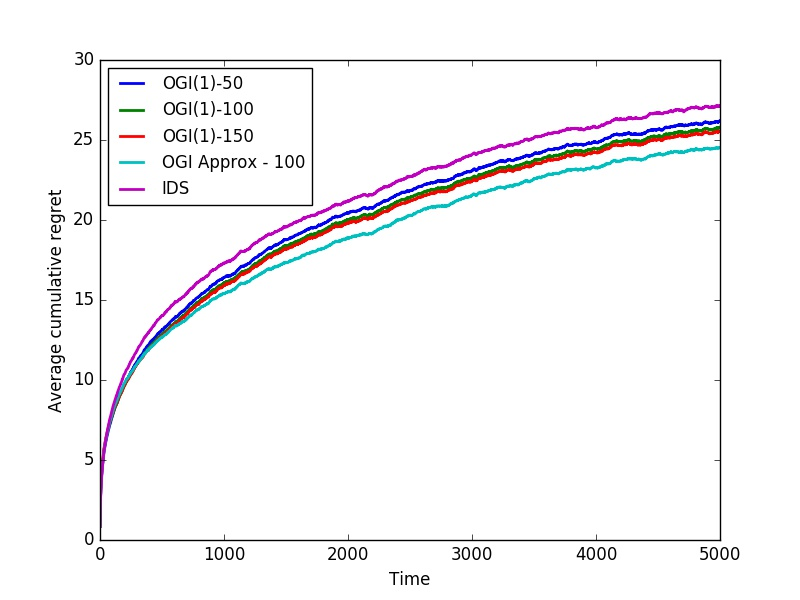
\includegraphics[width=\linewidth]{plots/reduced_gaussian_a.jpg}
		\caption{Gaussian experiment}
		\label{fig:sub1}
	\end{subfigure}
	\begin{subfigure}{.5\textwidth}
		\centering
		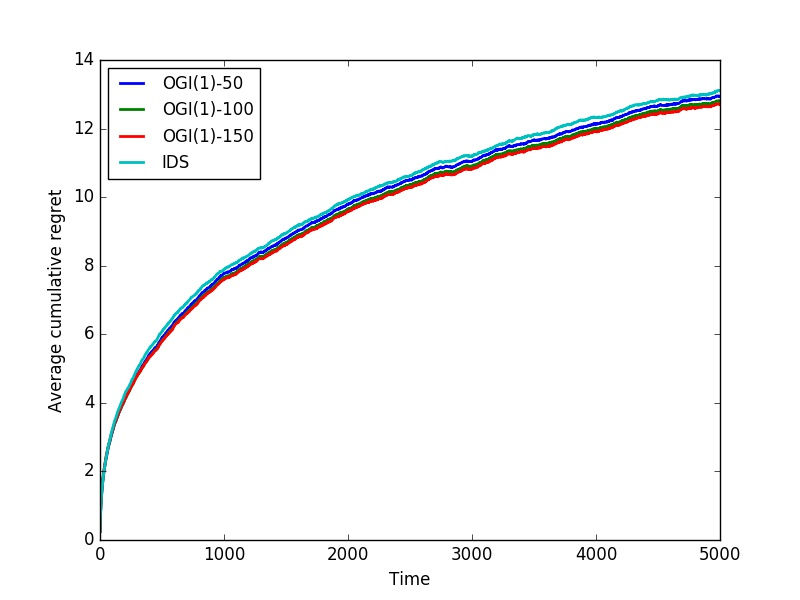
\includegraphics[width=\linewidth]{plots/reduced_figure_a.jpg}
		\caption{Bernoulli experiment}
		\label{fig:sub2}
	\end{subfigure}%
	\caption{Bayesian regret. In the legend, OGI($K$)-$\alpha$ is the format used to indicate parameters $K$ and $\alpha$. The OGI Approx policy uses the approximation to the Gittins index from \cite{powell2012optimal}.}
	\label{fig:bayesian_regret}
\end{figure}

In the Bernoulli experiment of this section, due to the computational cost, we are only able to simulate OGI with $K = 1$ lookahead steps. In addition, to show robustness with respect to the choice of tuning parameter $\alpha$, we show results for $\alpha = 50,100,150$. The message here is essentially the same as in the earlier experiments: the OGI scheme offers a non-trivial performance improvement at a tiny fraction of the computational effort required by its nearest competitor. We omit Thompson Sampling and Bayes UCB from the plots in order to more clearly see the difference between OGI and IDS.

In the Gaussian experiment, we again see that OGI dominates other policies and the tuning parameter has the same effect of lowering regret as it's increased. Also, just as in Table~\ref{table:gaussian_experiment1}, the OGI algorithm that uses the Gaussian-specific approximation has the best performance. 

\subsection{Thompson Sampling experiment} \label{exp:ts_sampling_experiment}
These experiments are motivated by similar ones in \cite{chapelle2011empirical}. The key feature here is that we simulate a longer horizon of $T = 10^6$ and include a greater number of arms, particularly we let $A \in \{10,40,70,100\}$. Since these experiments require substantially more iterations than the earlier ones, we are only able to simulate the fastest algorithms, which are OGI with $K=1$, Thompson Sampling and Bayes UCB. Again, this is a Bernoulli experiment where arm means are independently sampled from a uniform prior. The results are shown in Figure~\ref{fig:chapelle_and_li} with additional tables in Appendix~\ref{sec:further_exp}.
\begin{figure}
	\centering
	%% Creator: Matplotlib, PGF backend
%%
%% To include the figure in your LaTeX document, write
%%   \input{<filename>.pgf}
%%
%% Make sure the required packages are loaded in your preamble
%%   \usepackage{pgf}
%%
%% Figures using additional raster images can only be included by \input if
%% they are in the same directory as the main LaTeX file. For loading figures
%% from other directories you can use the `import` package
%%   \usepackage{import}
%% and then include the figures with
%%   \import{<path to file>}{<filename>.pgf}
%%
%% Matplotlib used the following preamble
%%   \usepackage[utf8x]{inputenc}
%%   \usepackage[T1]{fontenc}
%%
\begingroup%
\makeatletter%
\begin{pgfpicture}%
\pgfpathrectangle{\pgfpointorigin}{\pgfqpoint{6.500000in}{4.017221in}}%
\pgfusepath{use as bounding box, clip}%
\begin{pgfscope}%
\pgfsetbuttcap%
\pgfsetmiterjoin%
\definecolor{currentfill}{rgb}{1.000000,1.000000,1.000000}%
\pgfsetfillcolor{currentfill}%
\pgfsetlinewidth{0.000000pt}%
\definecolor{currentstroke}{rgb}{1.000000,1.000000,1.000000}%
\pgfsetstrokecolor{currentstroke}%
\pgfsetdash{}{0pt}%
\pgfpathmoveto{\pgfqpoint{0.000000in}{0.000000in}}%
\pgfpathlineto{\pgfqpoint{6.500000in}{0.000000in}}%
\pgfpathlineto{\pgfqpoint{6.500000in}{4.017221in}}%
\pgfpathlineto{\pgfqpoint{0.000000in}{4.017221in}}%
\pgfpathclose%
\pgfusepath{fill}%
\end{pgfscope}%
\begin{pgfscope}%
\pgfsetbuttcap%
\pgfsetmiterjoin%
\definecolor{currentfill}{rgb}{1.000000,1.000000,1.000000}%
\pgfsetfillcolor{currentfill}%
\pgfsetlinewidth{0.000000pt}%
\definecolor{currentstroke}{rgb}{0.000000,0.000000,0.000000}%
\pgfsetstrokecolor{currentstroke}%
\pgfsetstrokeopacity{0.000000}%
\pgfsetdash{}{0pt}%
\pgfpathmoveto{\pgfqpoint{0.574420in}{2.403614in}}%
\pgfpathlineto{\pgfqpoint{2.969172in}{2.403614in}}%
\pgfpathlineto{\pgfqpoint{2.969172in}{3.682468in}}%
\pgfpathlineto{\pgfqpoint{0.574420in}{3.682468in}}%
\pgfpathclose%
\pgfusepath{fill}%
\end{pgfscope}%
\begin{pgfscope}%
\pgfpathrectangle{\pgfqpoint{0.574420in}{2.403614in}}{\pgfqpoint{2.394752in}{1.278855in}} %
\pgfusepath{clip}%
\pgfsetrectcap%
\pgfsetroundjoin%
\pgfsetlinewidth{1.505625pt}%
\definecolor{currentstroke}{rgb}{0.000000,0.000000,1.000000}%
\pgfsetstrokecolor{currentstroke}%
\pgfsetdash{}{0pt}%
\pgfpathmoveto{\pgfqpoint{0.574422in}{2.407359in}}%
\pgfpathlineto{\pgfqpoint{0.598612in}{2.737596in}}%
\pgfpathlineto{\pgfqpoint{0.622801in}{2.806762in}}%
\pgfpathlineto{\pgfqpoint{0.646990in}{2.853506in}}%
\pgfpathlineto{\pgfqpoint{0.671180in}{2.882980in}}%
\pgfpathlineto{\pgfqpoint{0.695369in}{2.904819in}}%
\pgfpathlineto{\pgfqpoint{0.719559in}{2.928078in}}%
\pgfpathlineto{\pgfqpoint{0.743748in}{2.948701in}}%
\pgfpathlineto{\pgfqpoint{0.767937in}{2.967823in}}%
\pgfpathlineto{\pgfqpoint{0.792127in}{2.978093in}}%
\pgfpathlineto{\pgfqpoint{0.816316in}{2.993916in}}%
\pgfpathlineto{\pgfqpoint{0.840505in}{3.002459in}}%
\pgfpathlineto{\pgfqpoint{0.864695in}{3.011822in}}%
\pgfpathlineto{\pgfqpoint{0.888884in}{3.015944in}}%
\pgfpathlineto{\pgfqpoint{0.913074in}{3.028943in}}%
\pgfpathlineto{\pgfqpoint{0.937263in}{3.035855in}}%
\pgfpathlineto{\pgfqpoint{0.961452in}{3.040896in}}%
\pgfpathlineto{\pgfqpoint{0.985642in}{3.055161in}}%
\pgfpathlineto{\pgfqpoint{1.009831in}{3.056489in}}%
\pgfpathlineto{\pgfqpoint{1.034021in}{3.065877in}}%
\pgfpathlineto{\pgfqpoint{1.058210in}{3.071554in}}%
\pgfpathlineto{\pgfqpoint{1.082399in}{3.077109in}}%
\pgfpathlineto{\pgfqpoint{1.106589in}{3.084218in}}%
\pgfpathlineto{\pgfqpoint{1.130778in}{3.093544in}}%
\pgfpathlineto{\pgfqpoint{1.154968in}{3.094589in}}%
\pgfpathlineto{\pgfqpoint{1.179157in}{3.097676in}}%
\pgfpathlineto{\pgfqpoint{1.203346in}{3.098966in}}%
\pgfpathlineto{\pgfqpoint{1.227536in}{3.098744in}}%
\pgfpathlineto{\pgfqpoint{1.251725in}{3.096875in}}%
\pgfpathlineto{\pgfqpoint{1.275914in}{3.097778in}}%
\pgfpathlineto{\pgfqpoint{1.300104in}{3.104396in}}%
\pgfpathlineto{\pgfqpoint{1.324293in}{3.111683in}}%
\pgfpathlineto{\pgfqpoint{1.348483in}{3.116962in}}%
\pgfpathlineto{\pgfqpoint{1.372672in}{3.121948in}}%
\pgfpathlineto{\pgfqpoint{1.396861in}{3.131073in}}%
\pgfpathlineto{\pgfqpoint{1.421051in}{3.134912in}}%
\pgfpathlineto{\pgfqpoint{1.445240in}{3.139090in}}%
\pgfpathlineto{\pgfqpoint{1.469430in}{3.143766in}}%
\pgfpathlineto{\pgfqpoint{1.493619in}{3.153106in}}%
\pgfpathlineto{\pgfqpoint{1.517808in}{3.154818in}}%
\pgfpathlineto{\pgfqpoint{1.541998in}{3.156869in}}%
\pgfpathlineto{\pgfqpoint{1.566187in}{3.171038in}}%
\pgfpathlineto{\pgfqpoint{1.590377in}{3.174495in}}%
\pgfpathlineto{\pgfqpoint{1.614566in}{3.177220in}}%
\pgfpathlineto{\pgfqpoint{1.638755in}{3.179281in}}%
\pgfpathlineto{\pgfqpoint{1.662945in}{3.184693in}}%
\pgfpathlineto{\pgfqpoint{1.687134in}{3.188497in}}%
\pgfpathlineto{\pgfqpoint{1.711323in}{3.190996in}}%
\pgfpathlineto{\pgfqpoint{1.735513in}{3.200547in}}%
\pgfpathlineto{\pgfqpoint{1.759702in}{3.204345in}}%
\pgfpathlineto{\pgfqpoint{1.783892in}{3.207031in}}%
\pgfpathlineto{\pgfqpoint{1.808081in}{3.209673in}}%
\pgfpathlineto{\pgfqpoint{1.832270in}{3.210399in}}%
\pgfpathlineto{\pgfqpoint{1.856460in}{3.209800in}}%
\pgfpathlineto{\pgfqpoint{1.880649in}{3.214945in}}%
\pgfpathlineto{\pgfqpoint{1.904839in}{3.215450in}}%
\pgfpathlineto{\pgfqpoint{1.929028in}{3.213537in}}%
\pgfpathlineto{\pgfqpoint{1.953217in}{3.218229in}}%
\pgfpathlineto{\pgfqpoint{1.977407in}{3.222159in}}%
\pgfpathlineto{\pgfqpoint{2.001596in}{3.228387in}}%
\pgfpathlineto{\pgfqpoint{2.025786in}{3.230282in}}%
\pgfpathlineto{\pgfqpoint{2.049975in}{3.239513in}}%
\pgfpathlineto{\pgfqpoint{2.074164in}{3.243097in}}%
\pgfpathlineto{\pgfqpoint{2.098354in}{3.243272in}}%
\pgfpathlineto{\pgfqpoint{2.122543in}{3.243259in}}%
\pgfpathlineto{\pgfqpoint{2.146732in}{3.244581in}}%
\pgfpathlineto{\pgfqpoint{2.170922in}{3.247311in}}%
\pgfpathlineto{\pgfqpoint{2.195111in}{3.249309in}}%
\pgfpathlineto{\pgfqpoint{2.219301in}{3.251345in}}%
\pgfpathlineto{\pgfqpoint{2.243490in}{3.249506in}}%
\pgfpathlineto{\pgfqpoint{2.267679in}{3.252106in}}%
\pgfpathlineto{\pgfqpoint{2.291869in}{3.258762in}}%
\pgfpathlineto{\pgfqpoint{2.316058in}{3.265391in}}%
\pgfpathlineto{\pgfqpoint{2.340248in}{3.259718in}}%
\pgfpathlineto{\pgfqpoint{2.364437in}{3.256142in}}%
\pgfpathlineto{\pgfqpoint{2.388626in}{3.260395in}}%
\pgfpathlineto{\pgfqpoint{2.412816in}{3.262503in}}%
\pgfpathlineto{\pgfqpoint{2.437005in}{3.265894in}}%
\pgfpathlineto{\pgfqpoint{2.461195in}{3.260403in}}%
\pgfpathlineto{\pgfqpoint{2.485384in}{3.267467in}}%
\pgfpathlineto{\pgfqpoint{2.509573in}{3.276288in}}%
\pgfpathlineto{\pgfqpoint{2.533763in}{3.284975in}}%
\pgfpathlineto{\pgfqpoint{2.557952in}{3.282993in}}%
\pgfpathlineto{\pgfqpoint{2.582141in}{3.286156in}}%
\pgfpathlineto{\pgfqpoint{2.606331in}{3.289750in}}%
\pgfpathlineto{\pgfqpoint{2.630520in}{3.288344in}}%
\pgfpathlineto{\pgfqpoint{2.654710in}{3.289098in}}%
\pgfpathlineto{\pgfqpoint{2.678899in}{3.296418in}}%
\pgfpathlineto{\pgfqpoint{2.703088in}{3.307968in}}%
\pgfpathlineto{\pgfqpoint{2.727278in}{3.311121in}}%
\pgfpathlineto{\pgfqpoint{2.751467in}{3.312973in}}%
\pgfpathlineto{\pgfqpoint{2.775657in}{3.315752in}}%
\pgfpathlineto{\pgfqpoint{2.799846in}{3.313095in}}%
\pgfpathlineto{\pgfqpoint{2.824035in}{3.312444in}}%
\pgfpathlineto{\pgfqpoint{2.848225in}{3.316898in}}%
\pgfpathlineto{\pgfqpoint{2.872414in}{3.318239in}}%
\pgfpathlineto{\pgfqpoint{2.896604in}{3.313603in}}%
\pgfpathlineto{\pgfqpoint{2.920793in}{3.317808in}}%
\pgfpathlineto{\pgfqpoint{2.944982in}{3.323706in}}%
\pgfpathlineto{\pgfqpoint{2.969172in}{3.314286in}}%
\pgfusepath{stroke}%
\end{pgfscope}%
\begin{pgfscope}%
\pgfpathrectangle{\pgfqpoint{0.574420in}{2.403614in}}{\pgfqpoint{2.394752in}{1.278855in}} %
\pgfusepath{clip}%
\pgfsetrectcap%
\pgfsetroundjoin%
\pgfsetlinewidth{1.505625pt}%
\definecolor{currentstroke}{rgb}{0.000000,0.500000,0.000000}%
\pgfsetstrokecolor{currentstroke}%
\pgfsetdash{}{0pt}%
\pgfpathmoveto{\pgfqpoint{0.574422in}{2.407359in}}%
\pgfpathlineto{\pgfqpoint{0.598612in}{2.820913in}}%
\pgfpathlineto{\pgfqpoint{0.622801in}{2.882694in}}%
\pgfpathlineto{\pgfqpoint{0.646990in}{2.921998in}}%
\pgfpathlineto{\pgfqpoint{0.671180in}{2.947915in}}%
\pgfpathlineto{\pgfqpoint{0.695369in}{2.965891in}}%
\pgfpathlineto{\pgfqpoint{0.719559in}{2.986250in}}%
\pgfpathlineto{\pgfqpoint{0.743748in}{3.003615in}}%
\pgfpathlineto{\pgfqpoint{0.767937in}{3.020436in}}%
\pgfpathlineto{\pgfqpoint{0.792127in}{3.028596in}}%
\pgfpathlineto{\pgfqpoint{0.816316in}{3.041270in}}%
\pgfpathlineto{\pgfqpoint{0.840505in}{3.050967in}}%
\pgfpathlineto{\pgfqpoint{0.864695in}{3.061685in}}%
\pgfpathlineto{\pgfqpoint{0.888884in}{3.066072in}}%
\pgfpathlineto{\pgfqpoint{0.913074in}{3.078589in}}%
\pgfpathlineto{\pgfqpoint{0.937263in}{3.085501in}}%
\pgfpathlineto{\pgfqpoint{0.961452in}{3.090383in}}%
\pgfpathlineto{\pgfqpoint{0.985642in}{3.104677in}}%
\pgfpathlineto{\pgfqpoint{1.009831in}{3.105815in}}%
\pgfpathlineto{\pgfqpoint{1.034021in}{3.114599in}}%
\pgfpathlineto{\pgfqpoint{1.058210in}{3.118178in}}%
\pgfpathlineto{\pgfqpoint{1.082399in}{3.123440in}}%
\pgfpathlineto{\pgfqpoint{1.106589in}{3.130853in}}%
\pgfpathlineto{\pgfqpoint{1.130778in}{3.140747in}}%
\pgfpathlineto{\pgfqpoint{1.154968in}{3.141106in}}%
\pgfpathlineto{\pgfqpoint{1.179157in}{3.144760in}}%
\pgfpathlineto{\pgfqpoint{1.203346in}{3.146478in}}%
\pgfpathlineto{\pgfqpoint{1.227536in}{3.145001in}}%
\pgfpathlineto{\pgfqpoint{1.251725in}{3.143677in}}%
\pgfpathlineto{\pgfqpoint{1.275914in}{3.144919in}}%
\pgfpathlineto{\pgfqpoint{1.300104in}{3.151384in}}%
\pgfpathlineto{\pgfqpoint{1.324293in}{3.158139in}}%
\pgfpathlineto{\pgfqpoint{1.348483in}{3.163596in}}%
\pgfpathlineto{\pgfqpoint{1.372672in}{3.168687in}}%
\pgfpathlineto{\pgfqpoint{1.396861in}{3.178499in}}%
\pgfpathlineto{\pgfqpoint{1.421051in}{3.182041in}}%
\pgfpathlineto{\pgfqpoint{1.445240in}{3.186048in}}%
\pgfpathlineto{\pgfqpoint{1.469430in}{3.190599in}}%
\pgfpathlineto{\pgfqpoint{1.493619in}{3.199907in}}%
\pgfpathlineto{\pgfqpoint{1.517808in}{3.201061in}}%
\pgfpathlineto{\pgfqpoint{1.541998in}{3.202903in}}%
\pgfpathlineto{\pgfqpoint{1.566187in}{3.216704in}}%
\pgfpathlineto{\pgfqpoint{1.590377in}{3.219285in}}%
\pgfpathlineto{\pgfqpoint{1.614566in}{3.222598in}}%
\pgfpathlineto{\pgfqpoint{1.638755in}{3.224543in}}%
\pgfpathlineto{\pgfqpoint{1.662945in}{3.230946in}}%
\pgfpathlineto{\pgfqpoint{1.687134in}{3.235265in}}%
\pgfpathlineto{\pgfqpoint{1.711323in}{3.237782in}}%
\pgfpathlineto{\pgfqpoint{1.735513in}{3.247178in}}%
\pgfpathlineto{\pgfqpoint{1.759702in}{3.251051in}}%
\pgfpathlineto{\pgfqpoint{1.783892in}{3.254084in}}%
\pgfpathlineto{\pgfqpoint{1.808081in}{3.256349in}}%
\pgfpathlineto{\pgfqpoint{1.832270in}{3.257293in}}%
\pgfpathlineto{\pgfqpoint{1.856460in}{3.256557in}}%
\pgfpathlineto{\pgfqpoint{1.880649in}{3.261630in}}%
\pgfpathlineto{\pgfqpoint{1.904839in}{3.261877in}}%
\pgfpathlineto{\pgfqpoint{1.929028in}{3.260063in}}%
\pgfpathlineto{\pgfqpoint{1.953217in}{3.264357in}}%
\pgfpathlineto{\pgfqpoint{1.977407in}{3.267679in}}%
\pgfpathlineto{\pgfqpoint{2.001596in}{3.273988in}}%
\pgfpathlineto{\pgfqpoint{2.025786in}{3.275577in}}%
\pgfpathlineto{\pgfqpoint{2.049975in}{3.283715in}}%
\pgfpathlineto{\pgfqpoint{2.074164in}{3.287360in}}%
\pgfpathlineto{\pgfqpoint{2.098354in}{3.287135in}}%
\pgfpathlineto{\pgfqpoint{2.122543in}{3.288139in}}%
\pgfpathlineto{\pgfqpoint{2.146732in}{3.288694in}}%
\pgfpathlineto{\pgfqpoint{2.170922in}{3.291349in}}%
\pgfpathlineto{\pgfqpoint{2.195111in}{3.293422in}}%
\pgfpathlineto{\pgfqpoint{2.219301in}{3.294767in}}%
\pgfpathlineto{\pgfqpoint{2.243490in}{3.292140in}}%
\pgfpathlineto{\pgfqpoint{2.267679in}{3.293050in}}%
\pgfpathlineto{\pgfqpoint{2.291869in}{3.299248in}}%
\pgfpathlineto{\pgfqpoint{2.316058in}{3.305257in}}%
\pgfpathlineto{\pgfqpoint{2.340248in}{3.299639in}}%
\pgfpathlineto{\pgfqpoint{2.364437in}{3.296030in}}%
\pgfpathlineto{\pgfqpoint{2.388626in}{3.299247in}}%
\pgfpathlineto{\pgfqpoint{2.412816in}{3.300672in}}%
\pgfpathlineto{\pgfqpoint{2.437005in}{3.302945in}}%
\pgfpathlineto{\pgfqpoint{2.461195in}{3.296391in}}%
\pgfpathlineto{\pgfqpoint{2.485384in}{3.302726in}}%
\pgfpathlineto{\pgfqpoint{2.509573in}{3.310660in}}%
\pgfpathlineto{\pgfqpoint{2.533763in}{3.318968in}}%
\pgfpathlineto{\pgfqpoint{2.557952in}{3.316713in}}%
\pgfpathlineto{\pgfqpoint{2.582141in}{3.319798in}}%
\pgfpathlineto{\pgfqpoint{2.606331in}{3.322667in}}%
\pgfpathlineto{\pgfqpoint{2.630520in}{3.321212in}}%
\pgfpathlineto{\pgfqpoint{2.654710in}{3.322532in}}%
\pgfpathlineto{\pgfqpoint{2.678899in}{3.330113in}}%
\pgfpathlineto{\pgfqpoint{2.703088in}{3.341117in}}%
\pgfpathlineto{\pgfqpoint{2.727278in}{3.344228in}}%
\pgfpathlineto{\pgfqpoint{2.751467in}{3.345388in}}%
\pgfpathlineto{\pgfqpoint{2.775657in}{3.347542in}}%
\pgfpathlineto{\pgfqpoint{2.799846in}{3.344007in}}%
\pgfpathlineto{\pgfqpoint{2.824035in}{3.342713in}}%
\pgfpathlineto{\pgfqpoint{2.848225in}{3.345450in}}%
\pgfpathlineto{\pgfqpoint{2.872414in}{3.346686in}}%
\pgfpathlineto{\pgfqpoint{2.896604in}{3.342624in}}%
\pgfpathlineto{\pgfqpoint{2.920793in}{3.345982in}}%
\pgfpathlineto{\pgfqpoint{2.944982in}{3.351933in}}%
\pgfpathlineto{\pgfqpoint{2.969172in}{3.341964in}}%
\pgfusepath{stroke}%
\end{pgfscope}%
\begin{pgfscope}%
\pgfpathrectangle{\pgfqpoint{0.574420in}{2.403614in}}{\pgfqpoint{2.394752in}{1.278855in}} %
\pgfusepath{clip}%
\pgfsetrectcap%
\pgfsetroundjoin%
\pgfsetlinewidth{1.505625pt}%
\definecolor{currentstroke}{rgb}{1.000000,0.000000,0.000000}%
\pgfsetstrokecolor{currentstroke}%
\pgfsetdash{}{0pt}%
\pgfpathmoveto{\pgfqpoint{0.574422in}{2.407359in}}%
\pgfpathlineto{\pgfqpoint{0.598612in}{2.836080in}}%
\pgfpathlineto{\pgfqpoint{0.622801in}{2.922876in}}%
\pgfpathlineto{\pgfqpoint{0.646990in}{2.978906in}}%
\pgfpathlineto{\pgfqpoint{0.671180in}{3.015455in}}%
\pgfpathlineto{\pgfqpoint{0.695369in}{3.042499in}}%
\pgfpathlineto{\pgfqpoint{0.719559in}{3.070189in}}%
\pgfpathlineto{\pgfqpoint{0.743748in}{3.094572in}}%
\pgfpathlineto{\pgfqpoint{0.767937in}{3.117480in}}%
\pgfpathlineto{\pgfqpoint{0.792127in}{3.131417in}}%
\pgfpathlineto{\pgfqpoint{0.816316in}{3.150426in}}%
\pgfpathlineto{\pgfqpoint{0.840505in}{3.163481in}}%
\pgfpathlineto{\pgfqpoint{0.864695in}{3.177346in}}%
\pgfpathlineto{\pgfqpoint{0.888884in}{3.186336in}}%
\pgfpathlineto{\pgfqpoint{0.913074in}{3.202796in}}%
\pgfpathlineto{\pgfqpoint{0.937263in}{3.213286in}}%
\pgfpathlineto{\pgfqpoint{0.961452in}{3.221406in}}%
\pgfpathlineto{\pgfqpoint{0.985642in}{3.238544in}}%
\pgfpathlineto{\pgfqpoint{1.009831in}{3.242196in}}%
\pgfpathlineto{\pgfqpoint{1.034021in}{3.254692in}}%
\pgfpathlineto{\pgfqpoint{1.058210in}{3.263296in}}%
\pgfpathlineto{\pgfqpoint{1.082399in}{3.272442in}}%
\pgfpathlineto{\pgfqpoint{1.106589in}{3.283155in}}%
\pgfpathlineto{\pgfqpoint{1.130778in}{3.295284in}}%
\pgfpathlineto{\pgfqpoint{1.154968in}{3.297553in}}%
\pgfpathlineto{\pgfqpoint{1.179157in}{3.303105in}}%
\pgfpathlineto{\pgfqpoint{1.203346in}{3.307583in}}%
\pgfpathlineto{\pgfqpoint{1.227536in}{3.308822in}}%
\pgfpathlineto{\pgfqpoint{1.251725in}{3.309525in}}%
\pgfpathlineto{\pgfqpoint{1.275914in}{3.311279in}}%
\pgfpathlineto{\pgfqpoint{1.300104in}{3.319914in}}%
\pgfpathlineto{\pgfqpoint{1.324293in}{3.329229in}}%
\pgfpathlineto{\pgfqpoint{1.348483in}{3.336879in}}%
\pgfpathlineto{\pgfqpoint{1.372672in}{3.343662in}}%
\pgfpathlineto{\pgfqpoint{1.396861in}{3.354495in}}%
\pgfpathlineto{\pgfqpoint{1.421051in}{3.358893in}}%
\pgfpathlineto{\pgfqpoint{1.445240in}{3.363976in}}%
\pgfpathlineto{\pgfqpoint{1.469430in}{3.370389in}}%
\pgfpathlineto{\pgfqpoint{1.493619in}{3.381375in}}%
\pgfpathlineto{\pgfqpoint{1.517808in}{3.385206in}}%
\pgfpathlineto{\pgfqpoint{1.541998in}{3.388644in}}%
\pgfpathlineto{\pgfqpoint{1.566187in}{3.404779in}}%
\pgfpathlineto{\pgfqpoint{1.590377in}{3.409597in}}%
\pgfpathlineto{\pgfqpoint{1.614566in}{3.414190in}}%
\pgfpathlineto{\pgfqpoint{1.638755in}{3.417172in}}%
\pgfpathlineto{\pgfqpoint{1.662945in}{3.424426in}}%
\pgfpathlineto{\pgfqpoint{1.687134in}{3.429580in}}%
\pgfpathlineto{\pgfqpoint{1.711323in}{3.433972in}}%
\pgfpathlineto{\pgfqpoint{1.735513in}{3.444978in}}%
\pgfpathlineto{\pgfqpoint{1.759702in}{3.449346in}}%
\pgfpathlineto{\pgfqpoint{1.783892in}{3.453291in}}%
\pgfpathlineto{\pgfqpoint{1.808081in}{3.456377in}}%
\pgfpathlineto{\pgfqpoint{1.832270in}{3.457973in}}%
\pgfpathlineto{\pgfqpoint{1.856460in}{3.457956in}}%
\pgfpathlineto{\pgfqpoint{1.880649in}{3.464812in}}%
\pgfpathlineto{\pgfqpoint{1.904839in}{3.465639in}}%
\pgfpathlineto{\pgfqpoint{1.929028in}{3.463859in}}%
\pgfpathlineto{\pgfqpoint{1.953217in}{3.469450in}}%
\pgfpathlineto{\pgfqpoint{1.977407in}{3.473385in}}%
\pgfpathlineto{\pgfqpoint{2.001596in}{3.481518in}}%
\pgfpathlineto{\pgfqpoint{2.025786in}{3.484620in}}%
\pgfpathlineto{\pgfqpoint{2.049975in}{3.493880in}}%
\pgfpathlineto{\pgfqpoint{2.074164in}{3.498381in}}%
\pgfpathlineto{\pgfqpoint{2.098354in}{3.499208in}}%
\pgfpathlineto{\pgfqpoint{2.122543in}{3.500280in}}%
\pgfpathlineto{\pgfqpoint{2.146732in}{3.501946in}}%
\pgfpathlineto{\pgfqpoint{2.170922in}{3.505364in}}%
\pgfpathlineto{\pgfqpoint{2.195111in}{3.508145in}}%
\pgfpathlineto{\pgfqpoint{2.219301in}{3.510708in}}%
\pgfpathlineto{\pgfqpoint{2.243490in}{3.508403in}}%
\pgfpathlineto{\pgfqpoint{2.267679in}{3.511504in}}%
\pgfpathlineto{\pgfqpoint{2.291869in}{3.518407in}}%
\pgfpathlineto{\pgfqpoint{2.316058in}{3.525238in}}%
\pgfpathlineto{\pgfqpoint{2.340248in}{3.520608in}}%
\pgfpathlineto{\pgfqpoint{2.364437in}{3.517983in}}%
\pgfpathlineto{\pgfqpoint{2.388626in}{3.522107in}}%
\pgfpathlineto{\pgfqpoint{2.412816in}{3.524522in}}%
\pgfpathlineto{\pgfqpoint{2.437005in}{3.527211in}}%
\pgfpathlineto{\pgfqpoint{2.461195in}{3.521307in}}%
\pgfpathlineto{\pgfqpoint{2.485384in}{3.528129in}}%
\pgfpathlineto{\pgfqpoint{2.509573in}{3.537088in}}%
\pgfpathlineto{\pgfqpoint{2.533763in}{3.545946in}}%
\pgfpathlineto{\pgfqpoint{2.557952in}{3.544469in}}%
\pgfpathlineto{\pgfqpoint{2.582141in}{3.547805in}}%
\pgfpathlineto{\pgfqpoint{2.606331in}{3.551255in}}%
\pgfpathlineto{\pgfqpoint{2.630520in}{3.550099in}}%
\pgfpathlineto{\pgfqpoint{2.654710in}{3.551197in}}%
\pgfpathlineto{\pgfqpoint{2.678899in}{3.558915in}}%
\pgfpathlineto{\pgfqpoint{2.703088in}{3.570001in}}%
\pgfpathlineto{\pgfqpoint{2.727278in}{3.573761in}}%
\pgfpathlineto{\pgfqpoint{2.751467in}{3.575686in}}%
\pgfpathlineto{\pgfqpoint{2.775657in}{3.578319in}}%
\pgfpathlineto{\pgfqpoint{2.799846in}{3.575879in}}%
\pgfpathlineto{\pgfqpoint{2.824035in}{3.574908in}}%
\pgfpathlineto{\pgfqpoint{2.848225in}{3.578257in}}%
\pgfpathlineto{\pgfqpoint{2.872414in}{3.580031in}}%
\pgfpathlineto{\pgfqpoint{2.896604in}{3.575705in}}%
\pgfpathlineto{\pgfqpoint{2.920793in}{3.580041in}}%
\pgfpathlineto{\pgfqpoint{2.944982in}{3.587066in}}%
\pgfpathlineto{\pgfqpoint{2.969172in}{3.577845in}}%
\pgfusepath{stroke}%
\end{pgfscope}%
\begin{pgfscope}%
\pgfsetrectcap%
\pgfsetmiterjoin%
\pgfsetlinewidth{1.003750pt}%
\definecolor{currentstroke}{rgb}{0.000000,0.000000,0.000000}%
\pgfsetstrokecolor{currentstroke}%
\pgfsetdash{}{0pt}%
\pgfpathmoveto{\pgfqpoint{0.574420in}{3.682468in}}%
\pgfpathlineto{\pgfqpoint{2.969172in}{3.682468in}}%
\pgfusepath{stroke}%
\end{pgfscope}%
\begin{pgfscope}%
\pgfsetrectcap%
\pgfsetmiterjoin%
\pgfsetlinewidth{1.003750pt}%
\definecolor{currentstroke}{rgb}{0.000000,0.000000,0.000000}%
\pgfsetstrokecolor{currentstroke}%
\pgfsetdash{}{0pt}%
\pgfpathmoveto{\pgfqpoint{2.969172in}{2.403614in}}%
\pgfpathlineto{\pgfqpoint{2.969172in}{3.682468in}}%
\pgfusepath{stroke}%
\end{pgfscope}%
\begin{pgfscope}%
\pgfsetrectcap%
\pgfsetmiterjoin%
\pgfsetlinewidth{1.003750pt}%
\definecolor{currentstroke}{rgb}{0.000000,0.000000,0.000000}%
\pgfsetstrokecolor{currentstroke}%
\pgfsetdash{}{0pt}%
\pgfpathmoveto{\pgfqpoint{0.574420in}{2.403614in}}%
\pgfpathlineto{\pgfqpoint{2.969172in}{2.403614in}}%
\pgfusepath{stroke}%
\end{pgfscope}%
\begin{pgfscope}%
\pgfsetrectcap%
\pgfsetmiterjoin%
\pgfsetlinewidth{1.003750pt}%
\definecolor{currentstroke}{rgb}{0.000000,0.000000,0.000000}%
\pgfsetstrokecolor{currentstroke}%
\pgfsetdash{}{0pt}%
\pgfpathmoveto{\pgfqpoint{0.574420in}{2.403614in}}%
\pgfpathlineto{\pgfqpoint{0.574420in}{3.682468in}}%
\pgfusepath{stroke}%
\end{pgfscope}%
\begin{pgfscope}%
\pgfsetbuttcap%
\pgfsetroundjoin%
\definecolor{currentfill}{rgb}{0.000000,0.000000,0.000000}%
\pgfsetfillcolor{currentfill}%
\pgfsetlinewidth{0.501875pt}%
\definecolor{currentstroke}{rgb}{0.000000,0.000000,0.000000}%
\pgfsetstrokecolor{currentstroke}%
\pgfsetdash{}{0pt}%
\pgfsys@defobject{currentmarker}{\pgfqpoint{0.000000in}{0.000000in}}{\pgfqpoint{0.000000in}{0.055556in}}{%
\pgfpathmoveto{\pgfqpoint{0.000000in}{0.000000in}}%
\pgfpathlineto{\pgfqpoint{0.000000in}{0.055556in}}%
\pgfusepath{stroke,fill}%
}%
\begin{pgfscope}%
\pgfsys@transformshift{0.574420in}{2.403614in}%
\pgfsys@useobject{currentmarker}{}%
\end{pgfscope}%
\end{pgfscope}%
\begin{pgfscope}%
\pgfsetbuttcap%
\pgfsetroundjoin%
\definecolor{currentfill}{rgb}{0.000000,0.000000,0.000000}%
\pgfsetfillcolor{currentfill}%
\pgfsetlinewidth{0.501875pt}%
\definecolor{currentstroke}{rgb}{0.000000,0.000000,0.000000}%
\pgfsetstrokecolor{currentstroke}%
\pgfsetdash{}{0pt}%
\pgfsys@defobject{currentmarker}{\pgfqpoint{0.000000in}{-0.055556in}}{\pgfqpoint{0.000000in}{0.000000in}}{%
\pgfpathmoveto{\pgfqpoint{0.000000in}{0.000000in}}%
\pgfpathlineto{\pgfqpoint{0.000000in}{-0.055556in}}%
\pgfusepath{stroke,fill}%
}%
\begin{pgfscope}%
\pgfsys@transformshift{0.574420in}{3.682468in}%
\pgfsys@useobject{currentmarker}{}%
\end{pgfscope}%
\end{pgfscope}%
\begin{pgfscope}%
\pgftext[x=0.574420in,y=2.348058in,,top]{\rmfamily\fontsize{8.000000}{9.600000}\selectfont \(\displaystyle 0\)}%
\end{pgfscope}%
\begin{pgfscope}%
\pgfsetbuttcap%
\pgfsetroundjoin%
\definecolor{currentfill}{rgb}{0.000000,0.000000,0.000000}%
\pgfsetfillcolor{currentfill}%
\pgfsetlinewidth{0.501875pt}%
\definecolor{currentstroke}{rgb}{0.000000,0.000000,0.000000}%
\pgfsetstrokecolor{currentstroke}%
\pgfsetdash{}{0pt}%
\pgfsys@defobject{currentmarker}{\pgfqpoint{0.000000in}{0.000000in}}{\pgfqpoint{0.000000in}{0.055556in}}{%
\pgfpathmoveto{\pgfqpoint{0.000000in}{0.000000in}}%
\pgfpathlineto{\pgfqpoint{0.000000in}{0.055556in}}%
\pgfusepath{stroke,fill}%
}%
\begin{pgfscope}%
\pgfsys@transformshift{1.053370in}{2.403614in}%
\pgfsys@useobject{currentmarker}{}%
\end{pgfscope}%
\end{pgfscope}%
\begin{pgfscope}%
\pgfsetbuttcap%
\pgfsetroundjoin%
\definecolor{currentfill}{rgb}{0.000000,0.000000,0.000000}%
\pgfsetfillcolor{currentfill}%
\pgfsetlinewidth{0.501875pt}%
\definecolor{currentstroke}{rgb}{0.000000,0.000000,0.000000}%
\pgfsetstrokecolor{currentstroke}%
\pgfsetdash{}{0pt}%
\pgfsys@defobject{currentmarker}{\pgfqpoint{0.000000in}{-0.055556in}}{\pgfqpoint{0.000000in}{0.000000in}}{%
\pgfpathmoveto{\pgfqpoint{0.000000in}{0.000000in}}%
\pgfpathlineto{\pgfqpoint{0.000000in}{-0.055556in}}%
\pgfusepath{stroke,fill}%
}%
\begin{pgfscope}%
\pgfsys@transformshift{1.053370in}{3.682468in}%
\pgfsys@useobject{currentmarker}{}%
\end{pgfscope}%
\end{pgfscope}%
\begin{pgfscope}%
\pgftext[x=1.053370in,y=2.348058in,,top]{\rmfamily\fontsize{8.000000}{9.600000}\selectfont \(\displaystyle 200000\)}%
\end{pgfscope}%
\begin{pgfscope}%
\pgfsetbuttcap%
\pgfsetroundjoin%
\definecolor{currentfill}{rgb}{0.000000,0.000000,0.000000}%
\pgfsetfillcolor{currentfill}%
\pgfsetlinewidth{0.501875pt}%
\definecolor{currentstroke}{rgb}{0.000000,0.000000,0.000000}%
\pgfsetstrokecolor{currentstroke}%
\pgfsetdash{}{0pt}%
\pgfsys@defobject{currentmarker}{\pgfqpoint{0.000000in}{0.000000in}}{\pgfqpoint{0.000000in}{0.055556in}}{%
\pgfpathmoveto{\pgfqpoint{0.000000in}{0.000000in}}%
\pgfpathlineto{\pgfqpoint{0.000000in}{0.055556in}}%
\pgfusepath{stroke,fill}%
}%
\begin{pgfscope}%
\pgfsys@transformshift{1.532321in}{2.403614in}%
\pgfsys@useobject{currentmarker}{}%
\end{pgfscope}%
\end{pgfscope}%
\begin{pgfscope}%
\pgfsetbuttcap%
\pgfsetroundjoin%
\definecolor{currentfill}{rgb}{0.000000,0.000000,0.000000}%
\pgfsetfillcolor{currentfill}%
\pgfsetlinewidth{0.501875pt}%
\definecolor{currentstroke}{rgb}{0.000000,0.000000,0.000000}%
\pgfsetstrokecolor{currentstroke}%
\pgfsetdash{}{0pt}%
\pgfsys@defobject{currentmarker}{\pgfqpoint{0.000000in}{-0.055556in}}{\pgfqpoint{0.000000in}{0.000000in}}{%
\pgfpathmoveto{\pgfqpoint{0.000000in}{0.000000in}}%
\pgfpathlineto{\pgfqpoint{0.000000in}{-0.055556in}}%
\pgfusepath{stroke,fill}%
}%
\begin{pgfscope}%
\pgfsys@transformshift{1.532321in}{3.682468in}%
\pgfsys@useobject{currentmarker}{}%
\end{pgfscope}%
\end{pgfscope}%
\begin{pgfscope}%
\pgftext[x=1.532321in,y=2.348058in,,top]{\rmfamily\fontsize{8.000000}{9.600000}\selectfont \(\displaystyle 400000\)}%
\end{pgfscope}%
\begin{pgfscope}%
\pgfsetbuttcap%
\pgfsetroundjoin%
\definecolor{currentfill}{rgb}{0.000000,0.000000,0.000000}%
\pgfsetfillcolor{currentfill}%
\pgfsetlinewidth{0.501875pt}%
\definecolor{currentstroke}{rgb}{0.000000,0.000000,0.000000}%
\pgfsetstrokecolor{currentstroke}%
\pgfsetdash{}{0pt}%
\pgfsys@defobject{currentmarker}{\pgfqpoint{0.000000in}{0.000000in}}{\pgfqpoint{0.000000in}{0.055556in}}{%
\pgfpathmoveto{\pgfqpoint{0.000000in}{0.000000in}}%
\pgfpathlineto{\pgfqpoint{0.000000in}{0.055556in}}%
\pgfusepath{stroke,fill}%
}%
\begin{pgfscope}%
\pgfsys@transformshift{2.011271in}{2.403614in}%
\pgfsys@useobject{currentmarker}{}%
\end{pgfscope}%
\end{pgfscope}%
\begin{pgfscope}%
\pgfsetbuttcap%
\pgfsetroundjoin%
\definecolor{currentfill}{rgb}{0.000000,0.000000,0.000000}%
\pgfsetfillcolor{currentfill}%
\pgfsetlinewidth{0.501875pt}%
\definecolor{currentstroke}{rgb}{0.000000,0.000000,0.000000}%
\pgfsetstrokecolor{currentstroke}%
\pgfsetdash{}{0pt}%
\pgfsys@defobject{currentmarker}{\pgfqpoint{0.000000in}{-0.055556in}}{\pgfqpoint{0.000000in}{0.000000in}}{%
\pgfpathmoveto{\pgfqpoint{0.000000in}{0.000000in}}%
\pgfpathlineto{\pgfqpoint{0.000000in}{-0.055556in}}%
\pgfusepath{stroke,fill}%
}%
\begin{pgfscope}%
\pgfsys@transformshift{2.011271in}{3.682468in}%
\pgfsys@useobject{currentmarker}{}%
\end{pgfscope}%
\end{pgfscope}%
\begin{pgfscope}%
\pgftext[x=2.011271in,y=2.348058in,,top]{\rmfamily\fontsize{8.000000}{9.600000}\selectfont \(\displaystyle 600000\)}%
\end{pgfscope}%
\begin{pgfscope}%
\pgfsetbuttcap%
\pgfsetroundjoin%
\definecolor{currentfill}{rgb}{0.000000,0.000000,0.000000}%
\pgfsetfillcolor{currentfill}%
\pgfsetlinewidth{0.501875pt}%
\definecolor{currentstroke}{rgb}{0.000000,0.000000,0.000000}%
\pgfsetstrokecolor{currentstroke}%
\pgfsetdash{}{0pt}%
\pgfsys@defobject{currentmarker}{\pgfqpoint{0.000000in}{0.000000in}}{\pgfqpoint{0.000000in}{0.055556in}}{%
\pgfpathmoveto{\pgfqpoint{0.000000in}{0.000000in}}%
\pgfpathlineto{\pgfqpoint{0.000000in}{0.055556in}}%
\pgfusepath{stroke,fill}%
}%
\begin{pgfscope}%
\pgfsys@transformshift{2.490221in}{2.403614in}%
\pgfsys@useobject{currentmarker}{}%
\end{pgfscope}%
\end{pgfscope}%
\begin{pgfscope}%
\pgfsetbuttcap%
\pgfsetroundjoin%
\definecolor{currentfill}{rgb}{0.000000,0.000000,0.000000}%
\pgfsetfillcolor{currentfill}%
\pgfsetlinewidth{0.501875pt}%
\definecolor{currentstroke}{rgb}{0.000000,0.000000,0.000000}%
\pgfsetstrokecolor{currentstroke}%
\pgfsetdash{}{0pt}%
\pgfsys@defobject{currentmarker}{\pgfqpoint{0.000000in}{-0.055556in}}{\pgfqpoint{0.000000in}{0.000000in}}{%
\pgfpathmoveto{\pgfqpoint{0.000000in}{0.000000in}}%
\pgfpathlineto{\pgfqpoint{0.000000in}{-0.055556in}}%
\pgfusepath{stroke,fill}%
}%
\begin{pgfscope}%
\pgfsys@transformshift{2.490221in}{3.682468in}%
\pgfsys@useobject{currentmarker}{}%
\end{pgfscope}%
\end{pgfscope}%
\begin{pgfscope}%
\pgftext[x=2.490221in,y=2.348058in,,top]{\rmfamily\fontsize{8.000000}{9.600000}\selectfont \(\displaystyle 800000\)}%
\end{pgfscope}%
\begin{pgfscope}%
\pgfsetbuttcap%
\pgfsetroundjoin%
\definecolor{currentfill}{rgb}{0.000000,0.000000,0.000000}%
\pgfsetfillcolor{currentfill}%
\pgfsetlinewidth{0.501875pt}%
\definecolor{currentstroke}{rgb}{0.000000,0.000000,0.000000}%
\pgfsetstrokecolor{currentstroke}%
\pgfsetdash{}{0pt}%
\pgfsys@defobject{currentmarker}{\pgfqpoint{0.000000in}{0.000000in}}{\pgfqpoint{0.000000in}{0.055556in}}{%
\pgfpathmoveto{\pgfqpoint{0.000000in}{0.000000in}}%
\pgfpathlineto{\pgfqpoint{0.000000in}{0.055556in}}%
\pgfusepath{stroke,fill}%
}%
\begin{pgfscope}%
\pgfsys@transformshift{2.969172in}{2.403614in}%
\pgfsys@useobject{currentmarker}{}%
\end{pgfscope}%
\end{pgfscope}%
\begin{pgfscope}%
\pgfsetbuttcap%
\pgfsetroundjoin%
\definecolor{currentfill}{rgb}{0.000000,0.000000,0.000000}%
\pgfsetfillcolor{currentfill}%
\pgfsetlinewidth{0.501875pt}%
\definecolor{currentstroke}{rgb}{0.000000,0.000000,0.000000}%
\pgfsetstrokecolor{currentstroke}%
\pgfsetdash{}{0pt}%
\pgfsys@defobject{currentmarker}{\pgfqpoint{0.000000in}{-0.055556in}}{\pgfqpoint{0.000000in}{0.000000in}}{%
\pgfpathmoveto{\pgfqpoint{0.000000in}{0.000000in}}%
\pgfpathlineto{\pgfqpoint{0.000000in}{-0.055556in}}%
\pgfusepath{stroke,fill}%
}%
\begin{pgfscope}%
\pgfsys@transformshift{2.969172in}{3.682468in}%
\pgfsys@useobject{currentmarker}{}%
\end{pgfscope}%
\end{pgfscope}%
\begin{pgfscope}%
\pgftext[x=2.969172in,y=2.348058in,,top]{\rmfamily\fontsize{8.000000}{9.600000}\selectfont \(\displaystyle 1000000\)}%
\end{pgfscope}%
\begin{pgfscope}%
\pgftext[x=1.771796in,y=2.180489in,,top]{\rmfamily\fontsize{10.000000}{12.000000}\selectfont \(\displaystyle T\)}%
\end{pgfscope}%
\begin{pgfscope}%
\pgfsetbuttcap%
\pgfsetroundjoin%
\definecolor{currentfill}{rgb}{0.000000,0.000000,0.000000}%
\pgfsetfillcolor{currentfill}%
\pgfsetlinewidth{0.501875pt}%
\definecolor{currentstroke}{rgb}{0.000000,0.000000,0.000000}%
\pgfsetstrokecolor{currentstroke}%
\pgfsetdash{}{0pt}%
\pgfsys@defobject{currentmarker}{\pgfqpoint{0.000000in}{0.000000in}}{\pgfqpoint{0.055556in}{0.000000in}}{%
\pgfpathmoveto{\pgfqpoint{0.000000in}{0.000000in}}%
\pgfpathlineto{\pgfqpoint{0.055556in}{0.000000in}}%
\pgfusepath{stroke,fill}%
}%
\begin{pgfscope}%
\pgfsys@transformshift{0.574420in}{2.403614in}%
\pgfsys@useobject{currentmarker}{}%
\end{pgfscope}%
\end{pgfscope}%
\begin{pgfscope}%
\pgfsetbuttcap%
\pgfsetroundjoin%
\definecolor{currentfill}{rgb}{0.000000,0.000000,0.000000}%
\pgfsetfillcolor{currentfill}%
\pgfsetlinewidth{0.501875pt}%
\definecolor{currentstroke}{rgb}{0.000000,0.000000,0.000000}%
\pgfsetstrokecolor{currentstroke}%
\pgfsetdash{}{0pt}%
\pgfsys@defobject{currentmarker}{\pgfqpoint{-0.055556in}{0.000000in}}{\pgfqpoint{0.000000in}{0.000000in}}{%
\pgfpathmoveto{\pgfqpoint{0.000000in}{0.000000in}}%
\pgfpathlineto{\pgfqpoint{-0.055556in}{0.000000in}}%
\pgfusepath{stroke,fill}%
}%
\begin{pgfscope}%
\pgfsys@transformshift{2.969172in}{2.403614in}%
\pgfsys@useobject{currentmarker}{}%
\end{pgfscope}%
\end{pgfscope}%
\begin{pgfscope}%
\pgftext[x=0.518864in,y=2.403614in,right,]{\rmfamily\fontsize{8.000000}{9.600000}\selectfont \(\displaystyle 0\)}%
\end{pgfscope}%
\begin{pgfscope}%
\pgfsetbuttcap%
\pgfsetroundjoin%
\definecolor{currentfill}{rgb}{0.000000,0.000000,0.000000}%
\pgfsetfillcolor{currentfill}%
\pgfsetlinewidth{0.501875pt}%
\definecolor{currentstroke}{rgb}{0.000000,0.000000,0.000000}%
\pgfsetstrokecolor{currentstroke}%
\pgfsetdash{}{0pt}%
\pgfsys@defobject{currentmarker}{\pgfqpoint{0.000000in}{0.000000in}}{\pgfqpoint{0.055556in}{0.000000in}}{%
\pgfpathmoveto{\pgfqpoint{0.000000in}{0.000000in}}%
\pgfpathlineto{\pgfqpoint{0.055556in}{0.000000in}}%
\pgfusepath{stroke,fill}%
}%
\begin{pgfscope}%
\pgfsys@transformshift{0.574420in}{2.586307in}%
\pgfsys@useobject{currentmarker}{}%
\end{pgfscope}%
\end{pgfscope}%
\begin{pgfscope}%
\pgfsetbuttcap%
\pgfsetroundjoin%
\definecolor{currentfill}{rgb}{0.000000,0.000000,0.000000}%
\pgfsetfillcolor{currentfill}%
\pgfsetlinewidth{0.501875pt}%
\definecolor{currentstroke}{rgb}{0.000000,0.000000,0.000000}%
\pgfsetstrokecolor{currentstroke}%
\pgfsetdash{}{0pt}%
\pgfsys@defobject{currentmarker}{\pgfqpoint{-0.055556in}{0.000000in}}{\pgfqpoint{0.000000in}{0.000000in}}{%
\pgfpathmoveto{\pgfqpoint{0.000000in}{0.000000in}}%
\pgfpathlineto{\pgfqpoint{-0.055556in}{0.000000in}}%
\pgfusepath{stroke,fill}%
}%
\begin{pgfscope}%
\pgfsys@transformshift{2.969172in}{2.586307in}%
\pgfsys@useobject{currentmarker}{}%
\end{pgfscope}%
\end{pgfscope}%
\begin{pgfscope}%
\pgftext[x=0.518864in,y=2.586307in,right,]{\rmfamily\fontsize{8.000000}{9.600000}\selectfont \(\displaystyle 20\)}%
\end{pgfscope}%
\begin{pgfscope}%
\pgfsetbuttcap%
\pgfsetroundjoin%
\definecolor{currentfill}{rgb}{0.000000,0.000000,0.000000}%
\pgfsetfillcolor{currentfill}%
\pgfsetlinewidth{0.501875pt}%
\definecolor{currentstroke}{rgb}{0.000000,0.000000,0.000000}%
\pgfsetstrokecolor{currentstroke}%
\pgfsetdash{}{0pt}%
\pgfsys@defobject{currentmarker}{\pgfqpoint{0.000000in}{0.000000in}}{\pgfqpoint{0.055556in}{0.000000in}}{%
\pgfpathmoveto{\pgfqpoint{0.000000in}{0.000000in}}%
\pgfpathlineto{\pgfqpoint{0.055556in}{0.000000in}}%
\pgfusepath{stroke,fill}%
}%
\begin{pgfscope}%
\pgfsys@transformshift{0.574420in}{2.769001in}%
\pgfsys@useobject{currentmarker}{}%
\end{pgfscope}%
\end{pgfscope}%
\begin{pgfscope}%
\pgfsetbuttcap%
\pgfsetroundjoin%
\definecolor{currentfill}{rgb}{0.000000,0.000000,0.000000}%
\pgfsetfillcolor{currentfill}%
\pgfsetlinewidth{0.501875pt}%
\definecolor{currentstroke}{rgb}{0.000000,0.000000,0.000000}%
\pgfsetstrokecolor{currentstroke}%
\pgfsetdash{}{0pt}%
\pgfsys@defobject{currentmarker}{\pgfqpoint{-0.055556in}{0.000000in}}{\pgfqpoint{0.000000in}{0.000000in}}{%
\pgfpathmoveto{\pgfqpoint{0.000000in}{0.000000in}}%
\pgfpathlineto{\pgfqpoint{-0.055556in}{0.000000in}}%
\pgfusepath{stroke,fill}%
}%
\begin{pgfscope}%
\pgfsys@transformshift{2.969172in}{2.769001in}%
\pgfsys@useobject{currentmarker}{}%
\end{pgfscope}%
\end{pgfscope}%
\begin{pgfscope}%
\pgftext[x=0.518864in,y=2.769001in,right,]{\rmfamily\fontsize{8.000000}{9.600000}\selectfont \(\displaystyle 40\)}%
\end{pgfscope}%
\begin{pgfscope}%
\pgfsetbuttcap%
\pgfsetroundjoin%
\definecolor{currentfill}{rgb}{0.000000,0.000000,0.000000}%
\pgfsetfillcolor{currentfill}%
\pgfsetlinewidth{0.501875pt}%
\definecolor{currentstroke}{rgb}{0.000000,0.000000,0.000000}%
\pgfsetstrokecolor{currentstroke}%
\pgfsetdash{}{0pt}%
\pgfsys@defobject{currentmarker}{\pgfqpoint{0.000000in}{0.000000in}}{\pgfqpoint{0.055556in}{0.000000in}}{%
\pgfpathmoveto{\pgfqpoint{0.000000in}{0.000000in}}%
\pgfpathlineto{\pgfqpoint{0.055556in}{0.000000in}}%
\pgfusepath{stroke,fill}%
}%
\begin{pgfscope}%
\pgfsys@transformshift{0.574420in}{2.951694in}%
\pgfsys@useobject{currentmarker}{}%
\end{pgfscope}%
\end{pgfscope}%
\begin{pgfscope}%
\pgfsetbuttcap%
\pgfsetroundjoin%
\definecolor{currentfill}{rgb}{0.000000,0.000000,0.000000}%
\pgfsetfillcolor{currentfill}%
\pgfsetlinewidth{0.501875pt}%
\definecolor{currentstroke}{rgb}{0.000000,0.000000,0.000000}%
\pgfsetstrokecolor{currentstroke}%
\pgfsetdash{}{0pt}%
\pgfsys@defobject{currentmarker}{\pgfqpoint{-0.055556in}{0.000000in}}{\pgfqpoint{0.000000in}{0.000000in}}{%
\pgfpathmoveto{\pgfqpoint{0.000000in}{0.000000in}}%
\pgfpathlineto{\pgfqpoint{-0.055556in}{0.000000in}}%
\pgfusepath{stroke,fill}%
}%
\begin{pgfscope}%
\pgfsys@transformshift{2.969172in}{2.951694in}%
\pgfsys@useobject{currentmarker}{}%
\end{pgfscope}%
\end{pgfscope}%
\begin{pgfscope}%
\pgftext[x=0.518864in,y=2.951694in,right,]{\rmfamily\fontsize{8.000000}{9.600000}\selectfont \(\displaystyle 60\)}%
\end{pgfscope}%
\begin{pgfscope}%
\pgfsetbuttcap%
\pgfsetroundjoin%
\definecolor{currentfill}{rgb}{0.000000,0.000000,0.000000}%
\pgfsetfillcolor{currentfill}%
\pgfsetlinewidth{0.501875pt}%
\definecolor{currentstroke}{rgb}{0.000000,0.000000,0.000000}%
\pgfsetstrokecolor{currentstroke}%
\pgfsetdash{}{0pt}%
\pgfsys@defobject{currentmarker}{\pgfqpoint{0.000000in}{0.000000in}}{\pgfqpoint{0.055556in}{0.000000in}}{%
\pgfpathmoveto{\pgfqpoint{0.000000in}{0.000000in}}%
\pgfpathlineto{\pgfqpoint{0.055556in}{0.000000in}}%
\pgfusepath{stroke,fill}%
}%
\begin{pgfscope}%
\pgfsys@transformshift{0.574420in}{3.134388in}%
\pgfsys@useobject{currentmarker}{}%
\end{pgfscope}%
\end{pgfscope}%
\begin{pgfscope}%
\pgfsetbuttcap%
\pgfsetroundjoin%
\definecolor{currentfill}{rgb}{0.000000,0.000000,0.000000}%
\pgfsetfillcolor{currentfill}%
\pgfsetlinewidth{0.501875pt}%
\definecolor{currentstroke}{rgb}{0.000000,0.000000,0.000000}%
\pgfsetstrokecolor{currentstroke}%
\pgfsetdash{}{0pt}%
\pgfsys@defobject{currentmarker}{\pgfqpoint{-0.055556in}{0.000000in}}{\pgfqpoint{0.000000in}{0.000000in}}{%
\pgfpathmoveto{\pgfqpoint{0.000000in}{0.000000in}}%
\pgfpathlineto{\pgfqpoint{-0.055556in}{0.000000in}}%
\pgfusepath{stroke,fill}%
}%
\begin{pgfscope}%
\pgfsys@transformshift{2.969172in}{3.134388in}%
\pgfsys@useobject{currentmarker}{}%
\end{pgfscope}%
\end{pgfscope}%
\begin{pgfscope}%
\pgftext[x=0.518864in,y=3.134388in,right,]{\rmfamily\fontsize{8.000000}{9.600000}\selectfont \(\displaystyle 80\)}%
\end{pgfscope}%
\begin{pgfscope}%
\pgfsetbuttcap%
\pgfsetroundjoin%
\definecolor{currentfill}{rgb}{0.000000,0.000000,0.000000}%
\pgfsetfillcolor{currentfill}%
\pgfsetlinewidth{0.501875pt}%
\definecolor{currentstroke}{rgb}{0.000000,0.000000,0.000000}%
\pgfsetstrokecolor{currentstroke}%
\pgfsetdash{}{0pt}%
\pgfsys@defobject{currentmarker}{\pgfqpoint{0.000000in}{0.000000in}}{\pgfqpoint{0.055556in}{0.000000in}}{%
\pgfpathmoveto{\pgfqpoint{0.000000in}{0.000000in}}%
\pgfpathlineto{\pgfqpoint{0.055556in}{0.000000in}}%
\pgfusepath{stroke,fill}%
}%
\begin{pgfscope}%
\pgfsys@transformshift{0.574420in}{3.317081in}%
\pgfsys@useobject{currentmarker}{}%
\end{pgfscope}%
\end{pgfscope}%
\begin{pgfscope}%
\pgfsetbuttcap%
\pgfsetroundjoin%
\definecolor{currentfill}{rgb}{0.000000,0.000000,0.000000}%
\pgfsetfillcolor{currentfill}%
\pgfsetlinewidth{0.501875pt}%
\definecolor{currentstroke}{rgb}{0.000000,0.000000,0.000000}%
\pgfsetstrokecolor{currentstroke}%
\pgfsetdash{}{0pt}%
\pgfsys@defobject{currentmarker}{\pgfqpoint{-0.055556in}{0.000000in}}{\pgfqpoint{0.000000in}{0.000000in}}{%
\pgfpathmoveto{\pgfqpoint{0.000000in}{0.000000in}}%
\pgfpathlineto{\pgfqpoint{-0.055556in}{0.000000in}}%
\pgfusepath{stroke,fill}%
}%
\begin{pgfscope}%
\pgfsys@transformshift{2.969172in}{3.317081in}%
\pgfsys@useobject{currentmarker}{}%
\end{pgfscope}%
\end{pgfscope}%
\begin{pgfscope}%
\pgftext[x=0.518864in,y=3.317081in,right,]{\rmfamily\fontsize{8.000000}{9.600000}\selectfont \(\displaystyle 100\)}%
\end{pgfscope}%
\begin{pgfscope}%
\pgfsetbuttcap%
\pgfsetroundjoin%
\definecolor{currentfill}{rgb}{0.000000,0.000000,0.000000}%
\pgfsetfillcolor{currentfill}%
\pgfsetlinewidth{0.501875pt}%
\definecolor{currentstroke}{rgb}{0.000000,0.000000,0.000000}%
\pgfsetstrokecolor{currentstroke}%
\pgfsetdash{}{0pt}%
\pgfsys@defobject{currentmarker}{\pgfqpoint{0.000000in}{0.000000in}}{\pgfqpoint{0.055556in}{0.000000in}}{%
\pgfpathmoveto{\pgfqpoint{0.000000in}{0.000000in}}%
\pgfpathlineto{\pgfqpoint{0.055556in}{0.000000in}}%
\pgfusepath{stroke,fill}%
}%
\begin{pgfscope}%
\pgfsys@transformshift{0.574420in}{3.499775in}%
\pgfsys@useobject{currentmarker}{}%
\end{pgfscope}%
\end{pgfscope}%
\begin{pgfscope}%
\pgfsetbuttcap%
\pgfsetroundjoin%
\definecolor{currentfill}{rgb}{0.000000,0.000000,0.000000}%
\pgfsetfillcolor{currentfill}%
\pgfsetlinewidth{0.501875pt}%
\definecolor{currentstroke}{rgb}{0.000000,0.000000,0.000000}%
\pgfsetstrokecolor{currentstroke}%
\pgfsetdash{}{0pt}%
\pgfsys@defobject{currentmarker}{\pgfqpoint{-0.055556in}{0.000000in}}{\pgfqpoint{0.000000in}{0.000000in}}{%
\pgfpathmoveto{\pgfqpoint{0.000000in}{0.000000in}}%
\pgfpathlineto{\pgfqpoint{-0.055556in}{0.000000in}}%
\pgfusepath{stroke,fill}%
}%
\begin{pgfscope}%
\pgfsys@transformshift{2.969172in}{3.499775in}%
\pgfsys@useobject{currentmarker}{}%
\end{pgfscope}%
\end{pgfscope}%
\begin{pgfscope}%
\pgftext[x=0.518864in,y=3.499775in,right,]{\rmfamily\fontsize{8.000000}{9.600000}\selectfont \(\displaystyle 120\)}%
\end{pgfscope}%
\begin{pgfscope}%
\pgfsetbuttcap%
\pgfsetroundjoin%
\definecolor{currentfill}{rgb}{0.000000,0.000000,0.000000}%
\pgfsetfillcolor{currentfill}%
\pgfsetlinewidth{0.501875pt}%
\definecolor{currentstroke}{rgb}{0.000000,0.000000,0.000000}%
\pgfsetstrokecolor{currentstroke}%
\pgfsetdash{}{0pt}%
\pgfsys@defobject{currentmarker}{\pgfqpoint{0.000000in}{0.000000in}}{\pgfqpoint{0.055556in}{0.000000in}}{%
\pgfpathmoveto{\pgfqpoint{0.000000in}{0.000000in}}%
\pgfpathlineto{\pgfqpoint{0.055556in}{0.000000in}}%
\pgfusepath{stroke,fill}%
}%
\begin{pgfscope}%
\pgfsys@transformshift{0.574420in}{3.682468in}%
\pgfsys@useobject{currentmarker}{}%
\end{pgfscope}%
\end{pgfscope}%
\begin{pgfscope}%
\pgfsetbuttcap%
\pgfsetroundjoin%
\definecolor{currentfill}{rgb}{0.000000,0.000000,0.000000}%
\pgfsetfillcolor{currentfill}%
\pgfsetlinewidth{0.501875pt}%
\definecolor{currentstroke}{rgb}{0.000000,0.000000,0.000000}%
\pgfsetstrokecolor{currentstroke}%
\pgfsetdash{}{0pt}%
\pgfsys@defobject{currentmarker}{\pgfqpoint{-0.055556in}{0.000000in}}{\pgfqpoint{0.000000in}{0.000000in}}{%
\pgfpathmoveto{\pgfqpoint{0.000000in}{0.000000in}}%
\pgfpathlineto{\pgfqpoint{-0.055556in}{0.000000in}}%
\pgfusepath{stroke,fill}%
}%
\begin{pgfscope}%
\pgfsys@transformshift{2.969172in}{3.682468in}%
\pgfsys@useobject{currentmarker}{}%
\end{pgfscope}%
\end{pgfscope}%
\begin{pgfscope}%
\pgftext[x=0.518864in,y=3.682468in,right,]{\rmfamily\fontsize{8.000000}{9.600000}\selectfont \(\displaystyle 140\)}%
\end{pgfscope}%
\begin{pgfscope}%
\pgftext[x=0.272334in,y=3.043041in,,bottom,rotate=90.000000]{\rmfamily\fontsize{10.000000}{12.000000}\selectfont Regret}%
\end{pgfscope}%
\begin{pgfscope}%
\pgftext[x=1.771796in,y=3.751913in,,base]{\rmfamily\fontsize{12.000000}{14.400000}\selectfont \(\displaystyle A = 10\)}%
\end{pgfscope}%
\begin{pgfscope}%
\pgfsetbuttcap%
\pgfsetmiterjoin%
\definecolor{currentfill}{rgb}{1.000000,1.000000,1.000000}%
\pgfsetfillcolor{currentfill}%
\pgfsetlinewidth{1.003750pt}%
\definecolor{currentstroke}{rgb}{0.000000,0.000000,0.000000}%
\pgfsetstrokecolor{currentstroke}%
\pgfsetdash{}{0pt}%
\pgfpathmoveto{\pgfqpoint{1.919780in}{2.459169in}}%
\pgfpathlineto{\pgfqpoint{2.913616in}{2.459169in}}%
\pgfpathlineto{\pgfqpoint{2.913616in}{2.957302in}}%
\pgfpathlineto{\pgfqpoint{1.919780in}{2.957302in}}%
\pgfpathclose%
\pgfusepath{stroke,fill}%
\end{pgfscope}%
\begin{pgfscope}%
\pgfsetrectcap%
\pgfsetroundjoin%
\pgfsetlinewidth{1.505625pt}%
\definecolor{currentstroke}{rgb}{0.000000,0.000000,1.000000}%
\pgfsetstrokecolor{currentstroke}%
\pgfsetdash{}{0pt}%
\pgfpathmoveto{\pgfqpoint{1.997557in}{2.873968in}}%
\pgfpathlineto{\pgfqpoint{2.153113in}{2.873968in}}%
\pgfusepath{stroke}%
\end{pgfscope}%
\begin{pgfscope}%
\pgftext[x=2.275335in,y=2.835079in,left,base]{\rmfamily\fontsize{8.000000}{9.600000}\selectfont OGI}%
\end{pgfscope}%
\begin{pgfscope}%
\pgfsetrectcap%
\pgfsetroundjoin%
\pgfsetlinewidth{1.505625pt}%
\definecolor{currentstroke}{rgb}{0.000000,0.500000,0.000000}%
\pgfsetstrokecolor{currentstroke}%
\pgfsetdash{}{0pt}%
\pgfpathmoveto{\pgfqpoint{1.997557in}{2.719035in}}%
\pgfpathlineto{\pgfqpoint{2.153113in}{2.719035in}}%
\pgfusepath{stroke}%
\end{pgfscope}%
\begin{pgfscope}%
\pgftext[x=2.275335in,y=2.680146in,left,base]{\rmfamily\fontsize{8.000000}{9.600000}\selectfont Thompson}%
\end{pgfscope}%
\begin{pgfscope}%
\pgfsetrectcap%
\pgfsetroundjoin%
\pgfsetlinewidth{1.505625pt}%
\definecolor{currentstroke}{rgb}{1.000000,0.000000,0.000000}%
\pgfsetstrokecolor{currentstroke}%
\pgfsetdash{}{0pt}%
\pgfpathmoveto{\pgfqpoint{1.997557in}{2.564102in}}%
\pgfpathlineto{\pgfqpoint{2.153113in}{2.564102in}}%
\pgfusepath{stroke}%
\end{pgfscope}%
\begin{pgfscope}%
\pgftext[x=2.275335in,y=2.525213in,left,base]{\rmfamily\fontsize{8.000000}{9.600000}\selectfont Bayes UCB}%
\end{pgfscope}%
\begin{pgfscope}%
\pgfsetbuttcap%
\pgfsetmiterjoin%
\definecolor{currentfill}{rgb}{1.000000,1.000000,1.000000}%
\pgfsetfillcolor{currentfill}%
\pgfsetlinewidth{0.000000pt}%
\definecolor{currentstroke}{rgb}{0.000000,0.000000,0.000000}%
\pgfsetstrokecolor{currentstroke}%
\pgfsetstrokeopacity{0.000000}%
\pgfsetdash{}{0pt}%
\pgfpathmoveto{\pgfqpoint{3.749420in}{2.403614in}}%
\pgfpathlineto{\pgfqpoint{6.144172in}{2.403614in}}%
\pgfpathlineto{\pgfqpoint{6.144172in}{3.682468in}}%
\pgfpathlineto{\pgfqpoint{3.749420in}{3.682468in}}%
\pgfpathclose%
\pgfusepath{fill}%
\end{pgfscope}%
\begin{pgfscope}%
\pgfpathrectangle{\pgfqpoint{3.749420in}{2.403614in}}{\pgfqpoint{2.394752in}{1.278855in}} %
\pgfusepath{clip}%
\pgfsetrectcap%
\pgfsetroundjoin%
\pgfsetlinewidth{1.505625pt}%
\definecolor{currentstroke}{rgb}{0.000000,0.000000,1.000000}%
\pgfsetstrokecolor{currentstroke}%
\pgfsetdash{}{0pt}%
\pgfpathmoveto{\pgfqpoint{3.749422in}{2.406068in}}%
\pgfpathlineto{\pgfqpoint{3.773612in}{2.777630in}}%
\pgfpathlineto{\pgfqpoint{3.797801in}{2.855226in}}%
\pgfpathlineto{\pgfqpoint{3.821990in}{2.902613in}}%
\pgfpathlineto{\pgfqpoint{3.846180in}{2.936320in}}%
\pgfpathlineto{\pgfqpoint{3.870369in}{2.963944in}}%
\pgfpathlineto{\pgfqpoint{3.894559in}{2.986020in}}%
\pgfpathlineto{\pgfqpoint{3.918748in}{3.002775in}}%
\pgfpathlineto{\pgfqpoint{3.942937in}{3.017674in}}%
\pgfpathlineto{\pgfqpoint{3.967127in}{3.031457in}}%
\pgfpathlineto{\pgfqpoint{3.991316in}{3.045609in}}%
\pgfpathlineto{\pgfqpoint{4.015505in}{3.056775in}}%
\pgfpathlineto{\pgfqpoint{4.039695in}{3.067671in}}%
\pgfpathlineto{\pgfqpoint{4.063884in}{3.077890in}}%
\pgfpathlineto{\pgfqpoint{4.088074in}{3.085581in}}%
\pgfpathlineto{\pgfqpoint{4.112263in}{3.091743in}}%
\pgfpathlineto{\pgfqpoint{4.136452in}{3.100062in}}%
\pgfpathlineto{\pgfqpoint{4.160642in}{3.109064in}}%
\pgfpathlineto{\pgfqpoint{4.184831in}{3.114693in}}%
\pgfpathlineto{\pgfqpoint{4.209021in}{3.122415in}}%
\pgfpathlineto{\pgfqpoint{4.233210in}{3.128685in}}%
\pgfpathlineto{\pgfqpoint{4.257399in}{3.135141in}}%
\pgfpathlineto{\pgfqpoint{4.281589in}{3.141204in}}%
\pgfpathlineto{\pgfqpoint{4.305778in}{3.145457in}}%
\pgfpathlineto{\pgfqpoint{4.329968in}{3.151944in}}%
\pgfpathlineto{\pgfqpoint{4.354157in}{3.154635in}}%
\pgfpathlineto{\pgfqpoint{4.378346in}{3.157609in}}%
\pgfpathlineto{\pgfqpoint{4.402536in}{3.164054in}}%
\pgfpathlineto{\pgfqpoint{4.426725in}{3.168826in}}%
\pgfpathlineto{\pgfqpoint{4.450914in}{3.173263in}}%
\pgfpathlineto{\pgfqpoint{4.475104in}{3.176697in}}%
\pgfpathlineto{\pgfqpoint{4.499293in}{3.180942in}}%
\pgfpathlineto{\pgfqpoint{4.523483in}{3.182685in}}%
\pgfpathlineto{\pgfqpoint{4.547672in}{3.187136in}}%
\pgfpathlineto{\pgfqpoint{4.571861in}{3.190121in}}%
\pgfpathlineto{\pgfqpoint{4.596051in}{3.193248in}}%
\pgfpathlineto{\pgfqpoint{4.620240in}{3.197211in}}%
\pgfpathlineto{\pgfqpoint{4.644430in}{3.201057in}}%
\pgfpathlineto{\pgfqpoint{4.668619in}{3.205565in}}%
\pgfpathlineto{\pgfqpoint{4.692808in}{3.207818in}}%
\pgfpathlineto{\pgfqpoint{4.716998in}{3.211233in}}%
\pgfpathlineto{\pgfqpoint{4.741187in}{3.216358in}}%
\pgfpathlineto{\pgfqpoint{4.765377in}{3.220294in}}%
\pgfpathlineto{\pgfqpoint{4.789566in}{3.221024in}}%
\pgfpathlineto{\pgfqpoint{4.813755in}{3.224818in}}%
\pgfpathlineto{\pgfqpoint{4.837945in}{3.227460in}}%
\pgfpathlineto{\pgfqpoint{4.862134in}{3.230540in}}%
\pgfpathlineto{\pgfqpoint{4.886323in}{3.235084in}}%
\pgfpathlineto{\pgfqpoint{4.910513in}{3.238785in}}%
\pgfpathlineto{\pgfqpoint{4.934702in}{3.241130in}}%
\pgfpathlineto{\pgfqpoint{4.958892in}{3.243415in}}%
\pgfpathlineto{\pgfqpoint{4.983081in}{3.248412in}}%
\pgfpathlineto{\pgfqpoint{5.007270in}{3.249728in}}%
\pgfpathlineto{\pgfqpoint{5.031460in}{3.252168in}}%
\pgfpathlineto{\pgfqpoint{5.055649in}{3.254163in}}%
\pgfpathlineto{\pgfqpoint{5.079839in}{3.257450in}}%
\pgfpathlineto{\pgfqpoint{5.104028in}{3.260598in}}%
\pgfpathlineto{\pgfqpoint{5.128217in}{3.262976in}}%
\pgfpathlineto{\pgfqpoint{5.152407in}{3.265524in}}%
\pgfpathlineto{\pgfqpoint{5.176596in}{3.266705in}}%
\pgfpathlineto{\pgfqpoint{5.200786in}{3.267940in}}%
\pgfpathlineto{\pgfqpoint{5.224975in}{3.270544in}}%
\pgfpathlineto{\pgfqpoint{5.249164in}{3.273158in}}%
\pgfpathlineto{\pgfqpoint{5.273354in}{3.275596in}}%
\pgfpathlineto{\pgfqpoint{5.297543in}{3.276455in}}%
\pgfpathlineto{\pgfqpoint{5.321732in}{3.279473in}}%
\pgfpathlineto{\pgfqpoint{5.345922in}{3.281051in}}%
\pgfpathlineto{\pgfqpoint{5.370111in}{3.282444in}}%
\pgfpathlineto{\pgfqpoint{5.394301in}{3.283719in}}%
\pgfpathlineto{\pgfqpoint{5.418490in}{3.284969in}}%
\pgfpathlineto{\pgfqpoint{5.442679in}{3.286664in}}%
\pgfpathlineto{\pgfqpoint{5.466869in}{3.290974in}}%
\pgfpathlineto{\pgfqpoint{5.491058in}{3.293277in}}%
\pgfpathlineto{\pgfqpoint{5.515248in}{3.294545in}}%
\pgfpathlineto{\pgfqpoint{5.539437in}{3.298197in}}%
\pgfpathlineto{\pgfqpoint{5.563626in}{3.301531in}}%
\pgfpathlineto{\pgfqpoint{5.587816in}{3.305182in}}%
\pgfpathlineto{\pgfqpoint{5.612005in}{3.307118in}}%
\pgfpathlineto{\pgfqpoint{5.636195in}{3.308618in}}%
\pgfpathlineto{\pgfqpoint{5.660384in}{3.311410in}}%
\pgfpathlineto{\pgfqpoint{5.684573in}{3.312410in}}%
\pgfpathlineto{\pgfqpoint{5.708763in}{3.314058in}}%
\pgfpathlineto{\pgfqpoint{5.732952in}{3.314919in}}%
\pgfpathlineto{\pgfqpoint{5.757141in}{3.317040in}}%
\pgfpathlineto{\pgfqpoint{5.781331in}{3.318750in}}%
\pgfpathlineto{\pgfqpoint{5.805520in}{3.320125in}}%
\pgfpathlineto{\pgfqpoint{5.829710in}{3.322229in}}%
\pgfpathlineto{\pgfqpoint{5.853899in}{3.323120in}}%
\pgfpathlineto{\pgfqpoint{5.878088in}{3.324845in}}%
\pgfpathlineto{\pgfqpoint{5.902278in}{3.326439in}}%
\pgfpathlineto{\pgfqpoint{5.926467in}{3.327532in}}%
\pgfpathlineto{\pgfqpoint{5.950657in}{3.330103in}}%
\pgfpathlineto{\pgfqpoint{5.974846in}{3.332434in}}%
\pgfpathlineto{\pgfqpoint{5.999035in}{3.335150in}}%
\pgfpathlineto{\pgfqpoint{6.023225in}{3.335534in}}%
\pgfpathlineto{\pgfqpoint{6.047414in}{3.336584in}}%
\pgfpathlineto{\pgfqpoint{6.071604in}{3.339157in}}%
\pgfpathlineto{\pgfqpoint{6.095793in}{3.342375in}}%
\pgfpathlineto{\pgfqpoint{6.119982in}{3.343113in}}%
\pgfpathlineto{\pgfqpoint{6.144172in}{3.345546in}}%
\pgfusepath{stroke}%
\end{pgfscope}%
\begin{pgfscope}%
\pgfpathrectangle{\pgfqpoint{3.749420in}{2.403614in}}{\pgfqpoint{2.394752in}{1.278855in}} %
\pgfusepath{clip}%
\pgfsetrectcap%
\pgfsetroundjoin%
\pgfsetlinewidth{1.505625pt}%
\definecolor{currentstroke}{rgb}{0.000000,0.500000,0.000000}%
\pgfsetstrokecolor{currentstroke}%
\pgfsetdash{}{0pt}%
\pgfpathmoveto{\pgfqpoint{3.749422in}{2.406068in}}%
\pgfpathlineto{\pgfqpoint{3.773612in}{2.933064in}}%
\pgfpathlineto{\pgfqpoint{3.797801in}{3.004256in}}%
\pgfpathlineto{\pgfqpoint{3.821990in}{3.046101in}}%
\pgfpathlineto{\pgfqpoint{3.846180in}{3.076626in}}%
\pgfpathlineto{\pgfqpoint{3.870369in}{3.101054in}}%
\pgfpathlineto{\pgfqpoint{3.894559in}{3.120278in}}%
\pgfpathlineto{\pgfqpoint{3.918748in}{3.136118in}}%
\pgfpathlineto{\pgfqpoint{3.942937in}{3.150035in}}%
\pgfpathlineto{\pgfqpoint{3.967127in}{3.162049in}}%
\pgfpathlineto{\pgfqpoint{3.991316in}{3.174460in}}%
\pgfpathlineto{\pgfqpoint{4.015505in}{3.185589in}}%
\pgfpathlineto{\pgfqpoint{4.039695in}{3.197224in}}%
\pgfpathlineto{\pgfqpoint{4.063884in}{3.207378in}}%
\pgfpathlineto{\pgfqpoint{4.088074in}{3.215563in}}%
\pgfpathlineto{\pgfqpoint{4.112263in}{3.221556in}}%
\pgfpathlineto{\pgfqpoint{4.136452in}{3.229281in}}%
\pgfpathlineto{\pgfqpoint{4.160642in}{3.238336in}}%
\pgfpathlineto{\pgfqpoint{4.184831in}{3.244034in}}%
\pgfpathlineto{\pgfqpoint{4.209021in}{3.251644in}}%
\pgfpathlineto{\pgfqpoint{4.233210in}{3.258066in}}%
\pgfpathlineto{\pgfqpoint{4.257399in}{3.264146in}}%
\pgfpathlineto{\pgfqpoint{4.281589in}{3.270099in}}%
\pgfpathlineto{\pgfqpoint{4.305778in}{3.273822in}}%
\pgfpathlineto{\pgfqpoint{4.329968in}{3.280081in}}%
\pgfpathlineto{\pgfqpoint{4.354157in}{3.283171in}}%
\pgfpathlineto{\pgfqpoint{4.378346in}{3.286337in}}%
\pgfpathlineto{\pgfqpoint{4.402536in}{3.292511in}}%
\pgfpathlineto{\pgfqpoint{4.426725in}{3.297645in}}%
\pgfpathlineto{\pgfqpoint{4.450914in}{3.301935in}}%
\pgfpathlineto{\pgfqpoint{4.475104in}{3.305270in}}%
\pgfpathlineto{\pgfqpoint{4.499293in}{3.309923in}}%
\pgfpathlineto{\pgfqpoint{4.523483in}{3.312167in}}%
\pgfpathlineto{\pgfqpoint{4.547672in}{3.317186in}}%
\pgfpathlineto{\pgfqpoint{4.571861in}{3.319832in}}%
\pgfpathlineto{\pgfqpoint{4.596051in}{3.323053in}}%
\pgfpathlineto{\pgfqpoint{4.620240in}{3.327187in}}%
\pgfpathlineto{\pgfqpoint{4.644430in}{3.330770in}}%
\pgfpathlineto{\pgfqpoint{4.668619in}{3.335377in}}%
\pgfpathlineto{\pgfqpoint{4.692808in}{3.337499in}}%
\pgfpathlineto{\pgfqpoint{4.716998in}{3.340694in}}%
\pgfpathlineto{\pgfqpoint{4.741187in}{3.345644in}}%
\pgfpathlineto{\pgfqpoint{4.765377in}{3.349415in}}%
\pgfpathlineto{\pgfqpoint{4.789566in}{3.350082in}}%
\pgfpathlineto{\pgfqpoint{4.813755in}{3.352969in}}%
\pgfpathlineto{\pgfqpoint{4.837945in}{3.354486in}}%
\pgfpathlineto{\pgfqpoint{4.862134in}{3.356924in}}%
\pgfpathlineto{\pgfqpoint{4.886323in}{3.360756in}}%
\pgfpathlineto{\pgfqpoint{4.910513in}{3.363397in}}%
\pgfpathlineto{\pgfqpoint{4.934702in}{3.365507in}}%
\pgfpathlineto{\pgfqpoint{4.958892in}{3.367443in}}%
\pgfpathlineto{\pgfqpoint{4.983081in}{3.371906in}}%
\pgfpathlineto{\pgfqpoint{5.007270in}{3.373007in}}%
\pgfpathlineto{\pgfqpoint{5.031460in}{3.375095in}}%
\pgfpathlineto{\pgfqpoint{5.055649in}{3.376822in}}%
\pgfpathlineto{\pgfqpoint{5.079839in}{3.379235in}}%
\pgfpathlineto{\pgfqpoint{5.104028in}{3.381928in}}%
\pgfpathlineto{\pgfqpoint{5.128217in}{3.383808in}}%
\pgfpathlineto{\pgfqpoint{5.152407in}{3.386158in}}%
\pgfpathlineto{\pgfqpoint{5.176596in}{3.386783in}}%
\pgfpathlineto{\pgfqpoint{5.200786in}{3.387919in}}%
\pgfpathlineto{\pgfqpoint{5.224975in}{3.390279in}}%
\pgfpathlineto{\pgfqpoint{5.249164in}{3.392553in}}%
\pgfpathlineto{\pgfqpoint{5.273354in}{3.394850in}}%
\pgfpathlineto{\pgfqpoint{5.297543in}{3.395540in}}%
\pgfpathlineto{\pgfqpoint{5.321732in}{3.398694in}}%
\pgfpathlineto{\pgfqpoint{5.345922in}{3.400314in}}%
\pgfpathlineto{\pgfqpoint{5.370111in}{3.401792in}}%
\pgfpathlineto{\pgfqpoint{5.394301in}{3.403039in}}%
\pgfpathlineto{\pgfqpoint{5.418490in}{3.404439in}}%
\pgfpathlineto{\pgfqpoint{5.442679in}{3.405961in}}%
\pgfpathlineto{\pgfqpoint{5.466869in}{3.410107in}}%
\pgfpathlineto{\pgfqpoint{5.491058in}{3.411986in}}%
\pgfpathlineto{\pgfqpoint{5.515248in}{3.412582in}}%
\pgfpathlineto{\pgfqpoint{5.539437in}{3.415932in}}%
\pgfpathlineto{\pgfqpoint{5.563626in}{3.418495in}}%
\pgfpathlineto{\pgfqpoint{5.587816in}{3.422176in}}%
\pgfpathlineto{\pgfqpoint{5.612005in}{3.423857in}}%
\pgfpathlineto{\pgfqpoint{5.636195in}{3.424650in}}%
\pgfpathlineto{\pgfqpoint{5.660384in}{3.426934in}}%
\pgfpathlineto{\pgfqpoint{5.684573in}{3.427813in}}%
\pgfpathlineto{\pgfqpoint{5.708763in}{3.428771in}}%
\pgfpathlineto{\pgfqpoint{5.732952in}{3.429243in}}%
\pgfpathlineto{\pgfqpoint{5.757141in}{3.430906in}}%
\pgfpathlineto{\pgfqpoint{5.781331in}{3.431919in}}%
\pgfpathlineto{\pgfqpoint{5.805520in}{3.433016in}}%
\pgfpathlineto{\pgfqpoint{5.829710in}{3.434711in}}%
\pgfpathlineto{\pgfqpoint{5.853899in}{3.435140in}}%
\pgfpathlineto{\pgfqpoint{5.878088in}{3.436771in}}%
\pgfpathlineto{\pgfqpoint{5.902278in}{3.437927in}}%
\pgfpathlineto{\pgfqpoint{5.926467in}{3.439149in}}%
\pgfpathlineto{\pgfqpoint{5.950657in}{3.440889in}}%
\pgfpathlineto{\pgfqpoint{5.974846in}{3.442419in}}%
\pgfpathlineto{\pgfqpoint{5.999035in}{3.444359in}}%
\pgfpathlineto{\pgfqpoint{6.023225in}{3.444215in}}%
\pgfpathlineto{\pgfqpoint{6.047414in}{3.444670in}}%
\pgfpathlineto{\pgfqpoint{6.071604in}{3.446919in}}%
\pgfpathlineto{\pgfqpoint{6.095793in}{3.449451in}}%
\pgfpathlineto{\pgfqpoint{6.119982in}{3.449996in}}%
\pgfpathlineto{\pgfqpoint{6.144172in}{3.452088in}}%
\pgfusepath{stroke}%
\end{pgfscope}%
\begin{pgfscope}%
\pgfpathrectangle{\pgfqpoint{3.749420in}{2.403614in}}{\pgfqpoint{2.394752in}{1.278855in}} %
\pgfusepath{clip}%
\pgfsetrectcap%
\pgfsetroundjoin%
\pgfsetlinewidth{1.505625pt}%
\definecolor{currentstroke}{rgb}{1.000000,0.000000,0.000000}%
\pgfsetstrokecolor{currentstroke}%
\pgfsetdash{}{0pt}%
\pgfpathmoveto{\pgfqpoint{3.749422in}{2.406068in}}%
\pgfpathlineto{\pgfqpoint{3.773612in}{2.898467in}}%
\pgfpathlineto{\pgfqpoint{3.797801in}{2.993191in}}%
\pgfpathlineto{\pgfqpoint{3.821990in}{3.049500in}}%
\pgfpathlineto{\pgfqpoint{3.846180in}{3.090753in}}%
\pgfpathlineto{\pgfqpoint{3.870369in}{3.123601in}}%
\pgfpathlineto{\pgfqpoint{3.894559in}{3.150303in}}%
\pgfpathlineto{\pgfqpoint{3.918748in}{3.171172in}}%
\pgfpathlineto{\pgfqpoint{3.942937in}{3.190521in}}%
\pgfpathlineto{\pgfqpoint{3.967127in}{3.206932in}}%
\pgfpathlineto{\pgfqpoint{3.991316in}{3.224286in}}%
\pgfpathlineto{\pgfqpoint{4.015505in}{3.239084in}}%
\pgfpathlineto{\pgfqpoint{4.039695in}{3.253716in}}%
\pgfpathlineto{\pgfqpoint{4.063884in}{3.266698in}}%
\pgfpathlineto{\pgfqpoint{4.088074in}{3.276801in}}%
\pgfpathlineto{\pgfqpoint{4.112263in}{3.285668in}}%
\pgfpathlineto{\pgfqpoint{4.136452in}{3.295649in}}%
\pgfpathlineto{\pgfqpoint{4.160642in}{3.306983in}}%
\pgfpathlineto{\pgfqpoint{4.184831in}{3.315205in}}%
\pgfpathlineto{\pgfqpoint{4.209021in}{3.325580in}}%
\pgfpathlineto{\pgfqpoint{4.233210in}{3.333395in}}%
\pgfpathlineto{\pgfqpoint{4.257399in}{3.341945in}}%
\pgfpathlineto{\pgfqpoint{4.281589in}{3.349404in}}%
\pgfpathlineto{\pgfqpoint{4.305778in}{3.355021in}}%
\pgfpathlineto{\pgfqpoint{4.329968in}{3.362889in}}%
\pgfpathlineto{\pgfqpoint{4.354157in}{3.367081in}}%
\pgfpathlineto{\pgfqpoint{4.378346in}{3.371355in}}%
\pgfpathlineto{\pgfqpoint{4.402536in}{3.379592in}}%
\pgfpathlineto{\pgfqpoint{4.426725in}{3.385774in}}%
\pgfpathlineto{\pgfqpoint{4.450914in}{3.391350in}}%
\pgfpathlineto{\pgfqpoint{4.475104in}{3.396278in}}%
\pgfpathlineto{\pgfqpoint{4.499293in}{3.401630in}}%
\pgfpathlineto{\pgfqpoint{4.523483in}{3.404721in}}%
\pgfpathlineto{\pgfqpoint{4.547672in}{3.410682in}}%
\pgfpathlineto{\pgfqpoint{4.571861in}{3.414672in}}%
\pgfpathlineto{\pgfqpoint{4.596051in}{3.418714in}}%
\pgfpathlineto{\pgfqpoint{4.620240in}{3.423535in}}%
\pgfpathlineto{\pgfqpoint{4.644430in}{3.428101in}}%
\pgfpathlineto{\pgfqpoint{4.668619in}{3.433789in}}%
\pgfpathlineto{\pgfqpoint{4.692808in}{3.436822in}}%
\pgfpathlineto{\pgfqpoint{4.716998in}{3.441374in}}%
\pgfpathlineto{\pgfqpoint{4.741187in}{3.447367in}}%
\pgfpathlineto{\pgfqpoint{4.765377in}{3.452430in}}%
\pgfpathlineto{\pgfqpoint{4.789566in}{3.453478in}}%
\pgfpathlineto{\pgfqpoint{4.813755in}{3.457510in}}%
\pgfpathlineto{\pgfqpoint{4.837945in}{3.460300in}}%
\pgfpathlineto{\pgfqpoint{4.862134in}{3.464044in}}%
\pgfpathlineto{\pgfqpoint{4.886323in}{3.468985in}}%
\pgfpathlineto{\pgfqpoint{4.910513in}{3.472697in}}%
\pgfpathlineto{\pgfqpoint{4.934702in}{3.475818in}}%
\pgfpathlineto{\pgfqpoint{4.958892in}{3.478379in}}%
\pgfpathlineto{\pgfqpoint{4.983081in}{3.483762in}}%
\pgfpathlineto{\pgfqpoint{5.007270in}{3.485281in}}%
\pgfpathlineto{\pgfqpoint{5.031460in}{3.487865in}}%
\pgfpathlineto{\pgfqpoint{5.055649in}{3.490395in}}%
\pgfpathlineto{\pgfqpoint{5.079839in}{3.493669in}}%
\pgfpathlineto{\pgfqpoint{5.104028in}{3.497084in}}%
\pgfpathlineto{\pgfqpoint{5.128217in}{3.499564in}}%
\pgfpathlineto{\pgfqpoint{5.152407in}{3.502452in}}%
\pgfpathlineto{\pgfqpoint{5.176596in}{3.504007in}}%
\pgfpathlineto{\pgfqpoint{5.200786in}{3.506014in}}%
\pgfpathlineto{\pgfqpoint{5.224975in}{3.508929in}}%
\pgfpathlineto{\pgfqpoint{5.249164in}{3.512107in}}%
\pgfpathlineto{\pgfqpoint{5.273354in}{3.515415in}}%
\pgfpathlineto{\pgfqpoint{5.297543in}{3.516818in}}%
\pgfpathlineto{\pgfqpoint{5.321732in}{3.520455in}}%
\pgfpathlineto{\pgfqpoint{5.345922in}{3.522491in}}%
\pgfpathlineto{\pgfqpoint{5.370111in}{3.524575in}}%
\pgfpathlineto{\pgfqpoint{5.394301in}{3.526348in}}%
\pgfpathlineto{\pgfqpoint{5.418490in}{3.528027in}}%
\pgfpathlineto{\pgfqpoint{5.442679in}{3.530071in}}%
\pgfpathlineto{\pgfqpoint{5.466869in}{3.534701in}}%
\pgfpathlineto{\pgfqpoint{5.491058in}{3.537365in}}%
\pgfpathlineto{\pgfqpoint{5.515248in}{3.538910in}}%
\pgfpathlineto{\pgfqpoint{5.539437in}{3.542858in}}%
\pgfpathlineto{\pgfqpoint{5.563626in}{3.546281in}}%
\pgfpathlineto{\pgfqpoint{5.587816in}{3.550568in}}%
\pgfpathlineto{\pgfqpoint{5.612005in}{3.552787in}}%
\pgfpathlineto{\pgfqpoint{5.636195in}{3.554318in}}%
\pgfpathlineto{\pgfqpoint{5.660384in}{3.557025in}}%
\pgfpathlineto{\pgfqpoint{5.684573in}{3.558472in}}%
\pgfpathlineto{\pgfqpoint{5.708763in}{3.559679in}}%
\pgfpathlineto{\pgfqpoint{5.732952in}{3.560698in}}%
\pgfpathlineto{\pgfqpoint{5.757141in}{3.562843in}}%
\pgfpathlineto{\pgfqpoint{5.781331in}{3.564347in}}%
\pgfpathlineto{\pgfqpoint{5.805520in}{3.566291in}}%
\pgfpathlineto{\pgfqpoint{5.829710in}{3.568416in}}%
\pgfpathlineto{\pgfqpoint{5.853899in}{3.569543in}}%
\pgfpathlineto{\pgfqpoint{5.878088in}{3.571540in}}%
\pgfpathlineto{\pgfqpoint{5.902278in}{3.573460in}}%
\pgfpathlineto{\pgfqpoint{5.926467in}{3.575092in}}%
\pgfpathlineto{\pgfqpoint{5.950657in}{3.577466in}}%
\pgfpathlineto{\pgfqpoint{5.974846in}{3.579600in}}%
\pgfpathlineto{\pgfqpoint{5.999035in}{3.582418in}}%
\pgfpathlineto{\pgfqpoint{6.023225in}{3.582331in}}%
\pgfpathlineto{\pgfqpoint{6.047414in}{3.583301in}}%
\pgfpathlineto{\pgfqpoint{6.071604in}{3.586193in}}%
\pgfpathlineto{\pgfqpoint{6.095793in}{3.589349in}}%
\pgfpathlineto{\pgfqpoint{6.119982in}{3.590265in}}%
\pgfpathlineto{\pgfqpoint{6.144172in}{3.593158in}}%
\pgfusepath{stroke}%
\end{pgfscope}%
\begin{pgfscope}%
\pgfsetrectcap%
\pgfsetmiterjoin%
\pgfsetlinewidth{1.003750pt}%
\definecolor{currentstroke}{rgb}{0.000000,0.000000,0.000000}%
\pgfsetstrokecolor{currentstroke}%
\pgfsetdash{}{0pt}%
\pgfpathmoveto{\pgfqpoint{3.749420in}{3.682468in}}%
\pgfpathlineto{\pgfqpoint{6.144172in}{3.682468in}}%
\pgfusepath{stroke}%
\end{pgfscope}%
\begin{pgfscope}%
\pgfsetrectcap%
\pgfsetmiterjoin%
\pgfsetlinewidth{1.003750pt}%
\definecolor{currentstroke}{rgb}{0.000000,0.000000,0.000000}%
\pgfsetstrokecolor{currentstroke}%
\pgfsetdash{}{0pt}%
\pgfpathmoveto{\pgfqpoint{6.144172in}{2.403614in}}%
\pgfpathlineto{\pgfqpoint{6.144172in}{3.682468in}}%
\pgfusepath{stroke}%
\end{pgfscope}%
\begin{pgfscope}%
\pgfsetrectcap%
\pgfsetmiterjoin%
\pgfsetlinewidth{1.003750pt}%
\definecolor{currentstroke}{rgb}{0.000000,0.000000,0.000000}%
\pgfsetstrokecolor{currentstroke}%
\pgfsetdash{}{0pt}%
\pgfpathmoveto{\pgfqpoint{3.749420in}{2.403614in}}%
\pgfpathlineto{\pgfqpoint{6.144172in}{2.403614in}}%
\pgfusepath{stroke}%
\end{pgfscope}%
\begin{pgfscope}%
\pgfsetrectcap%
\pgfsetmiterjoin%
\pgfsetlinewidth{1.003750pt}%
\definecolor{currentstroke}{rgb}{0.000000,0.000000,0.000000}%
\pgfsetstrokecolor{currentstroke}%
\pgfsetdash{}{0pt}%
\pgfpathmoveto{\pgfqpoint{3.749420in}{2.403614in}}%
\pgfpathlineto{\pgfqpoint{3.749420in}{3.682468in}}%
\pgfusepath{stroke}%
\end{pgfscope}%
\begin{pgfscope}%
\pgfsetbuttcap%
\pgfsetroundjoin%
\definecolor{currentfill}{rgb}{0.000000,0.000000,0.000000}%
\pgfsetfillcolor{currentfill}%
\pgfsetlinewidth{0.501875pt}%
\definecolor{currentstroke}{rgb}{0.000000,0.000000,0.000000}%
\pgfsetstrokecolor{currentstroke}%
\pgfsetdash{}{0pt}%
\pgfsys@defobject{currentmarker}{\pgfqpoint{0.000000in}{0.000000in}}{\pgfqpoint{0.000000in}{0.055556in}}{%
\pgfpathmoveto{\pgfqpoint{0.000000in}{0.000000in}}%
\pgfpathlineto{\pgfqpoint{0.000000in}{0.055556in}}%
\pgfusepath{stroke,fill}%
}%
\begin{pgfscope}%
\pgfsys@transformshift{3.749420in}{2.403614in}%
\pgfsys@useobject{currentmarker}{}%
\end{pgfscope}%
\end{pgfscope}%
\begin{pgfscope}%
\pgfsetbuttcap%
\pgfsetroundjoin%
\definecolor{currentfill}{rgb}{0.000000,0.000000,0.000000}%
\pgfsetfillcolor{currentfill}%
\pgfsetlinewidth{0.501875pt}%
\definecolor{currentstroke}{rgb}{0.000000,0.000000,0.000000}%
\pgfsetstrokecolor{currentstroke}%
\pgfsetdash{}{0pt}%
\pgfsys@defobject{currentmarker}{\pgfqpoint{0.000000in}{-0.055556in}}{\pgfqpoint{0.000000in}{0.000000in}}{%
\pgfpathmoveto{\pgfqpoint{0.000000in}{0.000000in}}%
\pgfpathlineto{\pgfqpoint{0.000000in}{-0.055556in}}%
\pgfusepath{stroke,fill}%
}%
\begin{pgfscope}%
\pgfsys@transformshift{3.749420in}{3.682468in}%
\pgfsys@useobject{currentmarker}{}%
\end{pgfscope}%
\end{pgfscope}%
\begin{pgfscope}%
\pgftext[x=3.749420in,y=2.348058in,,top]{\rmfamily\fontsize{8.000000}{9.600000}\selectfont \(\displaystyle 0\)}%
\end{pgfscope}%
\begin{pgfscope}%
\pgfsetbuttcap%
\pgfsetroundjoin%
\definecolor{currentfill}{rgb}{0.000000,0.000000,0.000000}%
\pgfsetfillcolor{currentfill}%
\pgfsetlinewidth{0.501875pt}%
\definecolor{currentstroke}{rgb}{0.000000,0.000000,0.000000}%
\pgfsetstrokecolor{currentstroke}%
\pgfsetdash{}{0pt}%
\pgfsys@defobject{currentmarker}{\pgfqpoint{0.000000in}{0.000000in}}{\pgfqpoint{0.000000in}{0.055556in}}{%
\pgfpathmoveto{\pgfqpoint{0.000000in}{0.000000in}}%
\pgfpathlineto{\pgfqpoint{0.000000in}{0.055556in}}%
\pgfusepath{stroke,fill}%
}%
\begin{pgfscope}%
\pgfsys@transformshift{4.228370in}{2.403614in}%
\pgfsys@useobject{currentmarker}{}%
\end{pgfscope}%
\end{pgfscope}%
\begin{pgfscope}%
\pgfsetbuttcap%
\pgfsetroundjoin%
\definecolor{currentfill}{rgb}{0.000000,0.000000,0.000000}%
\pgfsetfillcolor{currentfill}%
\pgfsetlinewidth{0.501875pt}%
\definecolor{currentstroke}{rgb}{0.000000,0.000000,0.000000}%
\pgfsetstrokecolor{currentstroke}%
\pgfsetdash{}{0pt}%
\pgfsys@defobject{currentmarker}{\pgfqpoint{0.000000in}{-0.055556in}}{\pgfqpoint{0.000000in}{0.000000in}}{%
\pgfpathmoveto{\pgfqpoint{0.000000in}{0.000000in}}%
\pgfpathlineto{\pgfqpoint{0.000000in}{-0.055556in}}%
\pgfusepath{stroke,fill}%
}%
\begin{pgfscope}%
\pgfsys@transformshift{4.228370in}{3.682468in}%
\pgfsys@useobject{currentmarker}{}%
\end{pgfscope}%
\end{pgfscope}%
\begin{pgfscope}%
\pgftext[x=4.228370in,y=2.348058in,,top]{\rmfamily\fontsize{8.000000}{9.600000}\selectfont \(\displaystyle 200000\)}%
\end{pgfscope}%
\begin{pgfscope}%
\pgfsetbuttcap%
\pgfsetroundjoin%
\definecolor{currentfill}{rgb}{0.000000,0.000000,0.000000}%
\pgfsetfillcolor{currentfill}%
\pgfsetlinewidth{0.501875pt}%
\definecolor{currentstroke}{rgb}{0.000000,0.000000,0.000000}%
\pgfsetstrokecolor{currentstroke}%
\pgfsetdash{}{0pt}%
\pgfsys@defobject{currentmarker}{\pgfqpoint{0.000000in}{0.000000in}}{\pgfqpoint{0.000000in}{0.055556in}}{%
\pgfpathmoveto{\pgfqpoint{0.000000in}{0.000000in}}%
\pgfpathlineto{\pgfqpoint{0.000000in}{0.055556in}}%
\pgfusepath{stroke,fill}%
}%
\begin{pgfscope}%
\pgfsys@transformshift{4.707321in}{2.403614in}%
\pgfsys@useobject{currentmarker}{}%
\end{pgfscope}%
\end{pgfscope}%
\begin{pgfscope}%
\pgfsetbuttcap%
\pgfsetroundjoin%
\definecolor{currentfill}{rgb}{0.000000,0.000000,0.000000}%
\pgfsetfillcolor{currentfill}%
\pgfsetlinewidth{0.501875pt}%
\definecolor{currentstroke}{rgb}{0.000000,0.000000,0.000000}%
\pgfsetstrokecolor{currentstroke}%
\pgfsetdash{}{0pt}%
\pgfsys@defobject{currentmarker}{\pgfqpoint{0.000000in}{-0.055556in}}{\pgfqpoint{0.000000in}{0.000000in}}{%
\pgfpathmoveto{\pgfqpoint{0.000000in}{0.000000in}}%
\pgfpathlineto{\pgfqpoint{0.000000in}{-0.055556in}}%
\pgfusepath{stroke,fill}%
}%
\begin{pgfscope}%
\pgfsys@transformshift{4.707321in}{3.682468in}%
\pgfsys@useobject{currentmarker}{}%
\end{pgfscope}%
\end{pgfscope}%
\begin{pgfscope}%
\pgftext[x=4.707321in,y=2.348058in,,top]{\rmfamily\fontsize{8.000000}{9.600000}\selectfont \(\displaystyle 400000\)}%
\end{pgfscope}%
\begin{pgfscope}%
\pgfsetbuttcap%
\pgfsetroundjoin%
\definecolor{currentfill}{rgb}{0.000000,0.000000,0.000000}%
\pgfsetfillcolor{currentfill}%
\pgfsetlinewidth{0.501875pt}%
\definecolor{currentstroke}{rgb}{0.000000,0.000000,0.000000}%
\pgfsetstrokecolor{currentstroke}%
\pgfsetdash{}{0pt}%
\pgfsys@defobject{currentmarker}{\pgfqpoint{0.000000in}{0.000000in}}{\pgfqpoint{0.000000in}{0.055556in}}{%
\pgfpathmoveto{\pgfqpoint{0.000000in}{0.000000in}}%
\pgfpathlineto{\pgfqpoint{0.000000in}{0.055556in}}%
\pgfusepath{stroke,fill}%
}%
\begin{pgfscope}%
\pgfsys@transformshift{5.186271in}{2.403614in}%
\pgfsys@useobject{currentmarker}{}%
\end{pgfscope}%
\end{pgfscope}%
\begin{pgfscope}%
\pgfsetbuttcap%
\pgfsetroundjoin%
\definecolor{currentfill}{rgb}{0.000000,0.000000,0.000000}%
\pgfsetfillcolor{currentfill}%
\pgfsetlinewidth{0.501875pt}%
\definecolor{currentstroke}{rgb}{0.000000,0.000000,0.000000}%
\pgfsetstrokecolor{currentstroke}%
\pgfsetdash{}{0pt}%
\pgfsys@defobject{currentmarker}{\pgfqpoint{0.000000in}{-0.055556in}}{\pgfqpoint{0.000000in}{0.000000in}}{%
\pgfpathmoveto{\pgfqpoint{0.000000in}{0.000000in}}%
\pgfpathlineto{\pgfqpoint{0.000000in}{-0.055556in}}%
\pgfusepath{stroke,fill}%
}%
\begin{pgfscope}%
\pgfsys@transformshift{5.186271in}{3.682468in}%
\pgfsys@useobject{currentmarker}{}%
\end{pgfscope}%
\end{pgfscope}%
\begin{pgfscope}%
\pgftext[x=5.186271in,y=2.348058in,,top]{\rmfamily\fontsize{8.000000}{9.600000}\selectfont \(\displaystyle 600000\)}%
\end{pgfscope}%
\begin{pgfscope}%
\pgfsetbuttcap%
\pgfsetroundjoin%
\definecolor{currentfill}{rgb}{0.000000,0.000000,0.000000}%
\pgfsetfillcolor{currentfill}%
\pgfsetlinewidth{0.501875pt}%
\definecolor{currentstroke}{rgb}{0.000000,0.000000,0.000000}%
\pgfsetstrokecolor{currentstroke}%
\pgfsetdash{}{0pt}%
\pgfsys@defobject{currentmarker}{\pgfqpoint{0.000000in}{0.000000in}}{\pgfqpoint{0.000000in}{0.055556in}}{%
\pgfpathmoveto{\pgfqpoint{0.000000in}{0.000000in}}%
\pgfpathlineto{\pgfqpoint{0.000000in}{0.055556in}}%
\pgfusepath{stroke,fill}%
}%
\begin{pgfscope}%
\pgfsys@transformshift{5.665221in}{2.403614in}%
\pgfsys@useobject{currentmarker}{}%
\end{pgfscope}%
\end{pgfscope}%
\begin{pgfscope}%
\pgfsetbuttcap%
\pgfsetroundjoin%
\definecolor{currentfill}{rgb}{0.000000,0.000000,0.000000}%
\pgfsetfillcolor{currentfill}%
\pgfsetlinewidth{0.501875pt}%
\definecolor{currentstroke}{rgb}{0.000000,0.000000,0.000000}%
\pgfsetstrokecolor{currentstroke}%
\pgfsetdash{}{0pt}%
\pgfsys@defobject{currentmarker}{\pgfqpoint{0.000000in}{-0.055556in}}{\pgfqpoint{0.000000in}{0.000000in}}{%
\pgfpathmoveto{\pgfqpoint{0.000000in}{0.000000in}}%
\pgfpathlineto{\pgfqpoint{0.000000in}{-0.055556in}}%
\pgfusepath{stroke,fill}%
}%
\begin{pgfscope}%
\pgfsys@transformshift{5.665221in}{3.682468in}%
\pgfsys@useobject{currentmarker}{}%
\end{pgfscope}%
\end{pgfscope}%
\begin{pgfscope}%
\pgftext[x=5.665221in,y=2.348058in,,top]{\rmfamily\fontsize{8.000000}{9.600000}\selectfont \(\displaystyle 800000\)}%
\end{pgfscope}%
\begin{pgfscope}%
\pgfsetbuttcap%
\pgfsetroundjoin%
\definecolor{currentfill}{rgb}{0.000000,0.000000,0.000000}%
\pgfsetfillcolor{currentfill}%
\pgfsetlinewidth{0.501875pt}%
\definecolor{currentstroke}{rgb}{0.000000,0.000000,0.000000}%
\pgfsetstrokecolor{currentstroke}%
\pgfsetdash{}{0pt}%
\pgfsys@defobject{currentmarker}{\pgfqpoint{0.000000in}{0.000000in}}{\pgfqpoint{0.000000in}{0.055556in}}{%
\pgfpathmoveto{\pgfqpoint{0.000000in}{0.000000in}}%
\pgfpathlineto{\pgfqpoint{0.000000in}{0.055556in}}%
\pgfusepath{stroke,fill}%
}%
\begin{pgfscope}%
\pgfsys@transformshift{6.144172in}{2.403614in}%
\pgfsys@useobject{currentmarker}{}%
\end{pgfscope}%
\end{pgfscope}%
\begin{pgfscope}%
\pgfsetbuttcap%
\pgfsetroundjoin%
\definecolor{currentfill}{rgb}{0.000000,0.000000,0.000000}%
\pgfsetfillcolor{currentfill}%
\pgfsetlinewidth{0.501875pt}%
\definecolor{currentstroke}{rgb}{0.000000,0.000000,0.000000}%
\pgfsetstrokecolor{currentstroke}%
\pgfsetdash{}{0pt}%
\pgfsys@defobject{currentmarker}{\pgfqpoint{0.000000in}{-0.055556in}}{\pgfqpoint{0.000000in}{0.000000in}}{%
\pgfpathmoveto{\pgfqpoint{0.000000in}{0.000000in}}%
\pgfpathlineto{\pgfqpoint{0.000000in}{-0.055556in}}%
\pgfusepath{stroke,fill}%
}%
\begin{pgfscope}%
\pgfsys@transformshift{6.144172in}{3.682468in}%
\pgfsys@useobject{currentmarker}{}%
\end{pgfscope}%
\end{pgfscope}%
\begin{pgfscope}%
\pgftext[x=6.144172in,y=2.348058in,,top]{\rmfamily\fontsize{8.000000}{9.600000}\selectfont \(\displaystyle 1000000\)}%
\end{pgfscope}%
\begin{pgfscope}%
\pgftext[x=4.946796in,y=2.180489in,,top]{\rmfamily\fontsize{10.000000}{12.000000}\selectfont \(\displaystyle T\)}%
\end{pgfscope}%
\begin{pgfscope}%
\pgfsetbuttcap%
\pgfsetroundjoin%
\definecolor{currentfill}{rgb}{0.000000,0.000000,0.000000}%
\pgfsetfillcolor{currentfill}%
\pgfsetlinewidth{0.501875pt}%
\definecolor{currentstroke}{rgb}{0.000000,0.000000,0.000000}%
\pgfsetstrokecolor{currentstroke}%
\pgfsetdash{}{0pt}%
\pgfsys@defobject{currentmarker}{\pgfqpoint{0.000000in}{0.000000in}}{\pgfqpoint{0.055556in}{0.000000in}}{%
\pgfpathmoveto{\pgfqpoint{0.000000in}{0.000000in}}%
\pgfpathlineto{\pgfqpoint{0.055556in}{0.000000in}}%
\pgfusepath{stroke,fill}%
}%
\begin{pgfscope}%
\pgfsys@transformshift{3.749420in}{2.403614in}%
\pgfsys@useobject{currentmarker}{}%
\end{pgfscope}%
\end{pgfscope}%
\begin{pgfscope}%
\pgfsetbuttcap%
\pgfsetroundjoin%
\definecolor{currentfill}{rgb}{0.000000,0.000000,0.000000}%
\pgfsetfillcolor{currentfill}%
\pgfsetlinewidth{0.501875pt}%
\definecolor{currentstroke}{rgb}{0.000000,0.000000,0.000000}%
\pgfsetstrokecolor{currentstroke}%
\pgfsetdash{}{0pt}%
\pgfsys@defobject{currentmarker}{\pgfqpoint{-0.055556in}{0.000000in}}{\pgfqpoint{0.000000in}{0.000000in}}{%
\pgfpathmoveto{\pgfqpoint{0.000000in}{0.000000in}}%
\pgfpathlineto{\pgfqpoint{-0.055556in}{0.000000in}}%
\pgfusepath{stroke,fill}%
}%
\begin{pgfscope}%
\pgfsys@transformshift{6.144172in}{2.403614in}%
\pgfsys@useobject{currentmarker}{}%
\end{pgfscope}%
\end{pgfscope}%
\begin{pgfscope}%
\pgftext[x=3.693864in,y=2.403614in,right,]{\rmfamily\fontsize{8.000000}{9.600000}\selectfont \(\displaystyle 0\)}%
\end{pgfscope}%
\begin{pgfscope}%
\pgfsetbuttcap%
\pgfsetroundjoin%
\definecolor{currentfill}{rgb}{0.000000,0.000000,0.000000}%
\pgfsetfillcolor{currentfill}%
\pgfsetlinewidth{0.501875pt}%
\definecolor{currentstroke}{rgb}{0.000000,0.000000,0.000000}%
\pgfsetstrokecolor{currentstroke}%
\pgfsetdash{}{0pt}%
\pgfsys@defobject{currentmarker}{\pgfqpoint{0.000000in}{0.000000in}}{\pgfqpoint{0.055556in}{0.000000in}}{%
\pgfpathmoveto{\pgfqpoint{0.000000in}{0.000000in}}%
\pgfpathlineto{\pgfqpoint{0.055556in}{0.000000in}}%
\pgfusepath{stroke,fill}%
}%
\begin{pgfscope}%
\pgfsys@transformshift{3.749420in}{2.659385in}%
\pgfsys@useobject{currentmarker}{}%
\end{pgfscope}%
\end{pgfscope}%
\begin{pgfscope}%
\pgfsetbuttcap%
\pgfsetroundjoin%
\definecolor{currentfill}{rgb}{0.000000,0.000000,0.000000}%
\pgfsetfillcolor{currentfill}%
\pgfsetlinewidth{0.501875pt}%
\definecolor{currentstroke}{rgb}{0.000000,0.000000,0.000000}%
\pgfsetstrokecolor{currentstroke}%
\pgfsetdash{}{0pt}%
\pgfsys@defobject{currentmarker}{\pgfqpoint{-0.055556in}{0.000000in}}{\pgfqpoint{0.000000in}{0.000000in}}{%
\pgfpathmoveto{\pgfqpoint{0.000000in}{0.000000in}}%
\pgfpathlineto{\pgfqpoint{-0.055556in}{0.000000in}}%
\pgfusepath{stroke,fill}%
}%
\begin{pgfscope}%
\pgfsys@transformshift{6.144172in}{2.659385in}%
\pgfsys@useobject{currentmarker}{}%
\end{pgfscope}%
\end{pgfscope}%
\begin{pgfscope}%
\pgftext[x=3.693864in,y=2.659385in,right,]{\rmfamily\fontsize{8.000000}{9.600000}\selectfont \(\displaystyle 50\)}%
\end{pgfscope}%
\begin{pgfscope}%
\pgfsetbuttcap%
\pgfsetroundjoin%
\definecolor{currentfill}{rgb}{0.000000,0.000000,0.000000}%
\pgfsetfillcolor{currentfill}%
\pgfsetlinewidth{0.501875pt}%
\definecolor{currentstroke}{rgb}{0.000000,0.000000,0.000000}%
\pgfsetstrokecolor{currentstroke}%
\pgfsetdash{}{0pt}%
\pgfsys@defobject{currentmarker}{\pgfqpoint{0.000000in}{0.000000in}}{\pgfqpoint{0.055556in}{0.000000in}}{%
\pgfpathmoveto{\pgfqpoint{0.000000in}{0.000000in}}%
\pgfpathlineto{\pgfqpoint{0.055556in}{0.000000in}}%
\pgfusepath{stroke,fill}%
}%
\begin{pgfscope}%
\pgfsys@transformshift{3.749420in}{2.915156in}%
\pgfsys@useobject{currentmarker}{}%
\end{pgfscope}%
\end{pgfscope}%
\begin{pgfscope}%
\pgfsetbuttcap%
\pgfsetroundjoin%
\definecolor{currentfill}{rgb}{0.000000,0.000000,0.000000}%
\pgfsetfillcolor{currentfill}%
\pgfsetlinewidth{0.501875pt}%
\definecolor{currentstroke}{rgb}{0.000000,0.000000,0.000000}%
\pgfsetstrokecolor{currentstroke}%
\pgfsetdash{}{0pt}%
\pgfsys@defobject{currentmarker}{\pgfqpoint{-0.055556in}{0.000000in}}{\pgfqpoint{0.000000in}{0.000000in}}{%
\pgfpathmoveto{\pgfqpoint{0.000000in}{0.000000in}}%
\pgfpathlineto{\pgfqpoint{-0.055556in}{0.000000in}}%
\pgfusepath{stroke,fill}%
}%
\begin{pgfscope}%
\pgfsys@transformshift{6.144172in}{2.915156in}%
\pgfsys@useobject{currentmarker}{}%
\end{pgfscope}%
\end{pgfscope}%
\begin{pgfscope}%
\pgftext[x=3.693864in,y=2.915156in,right,]{\rmfamily\fontsize{8.000000}{9.600000}\selectfont \(\displaystyle 100\)}%
\end{pgfscope}%
\begin{pgfscope}%
\pgfsetbuttcap%
\pgfsetroundjoin%
\definecolor{currentfill}{rgb}{0.000000,0.000000,0.000000}%
\pgfsetfillcolor{currentfill}%
\pgfsetlinewidth{0.501875pt}%
\definecolor{currentstroke}{rgb}{0.000000,0.000000,0.000000}%
\pgfsetstrokecolor{currentstroke}%
\pgfsetdash{}{0pt}%
\pgfsys@defobject{currentmarker}{\pgfqpoint{0.000000in}{0.000000in}}{\pgfqpoint{0.055556in}{0.000000in}}{%
\pgfpathmoveto{\pgfqpoint{0.000000in}{0.000000in}}%
\pgfpathlineto{\pgfqpoint{0.055556in}{0.000000in}}%
\pgfusepath{stroke,fill}%
}%
\begin{pgfscope}%
\pgfsys@transformshift{3.749420in}{3.170926in}%
\pgfsys@useobject{currentmarker}{}%
\end{pgfscope}%
\end{pgfscope}%
\begin{pgfscope}%
\pgfsetbuttcap%
\pgfsetroundjoin%
\definecolor{currentfill}{rgb}{0.000000,0.000000,0.000000}%
\pgfsetfillcolor{currentfill}%
\pgfsetlinewidth{0.501875pt}%
\definecolor{currentstroke}{rgb}{0.000000,0.000000,0.000000}%
\pgfsetstrokecolor{currentstroke}%
\pgfsetdash{}{0pt}%
\pgfsys@defobject{currentmarker}{\pgfqpoint{-0.055556in}{0.000000in}}{\pgfqpoint{0.000000in}{0.000000in}}{%
\pgfpathmoveto{\pgfqpoint{0.000000in}{0.000000in}}%
\pgfpathlineto{\pgfqpoint{-0.055556in}{0.000000in}}%
\pgfusepath{stroke,fill}%
}%
\begin{pgfscope}%
\pgfsys@transformshift{6.144172in}{3.170926in}%
\pgfsys@useobject{currentmarker}{}%
\end{pgfscope}%
\end{pgfscope}%
\begin{pgfscope}%
\pgftext[x=3.693864in,y=3.170926in,right,]{\rmfamily\fontsize{8.000000}{9.600000}\selectfont \(\displaystyle 150\)}%
\end{pgfscope}%
\begin{pgfscope}%
\pgfsetbuttcap%
\pgfsetroundjoin%
\definecolor{currentfill}{rgb}{0.000000,0.000000,0.000000}%
\pgfsetfillcolor{currentfill}%
\pgfsetlinewidth{0.501875pt}%
\definecolor{currentstroke}{rgb}{0.000000,0.000000,0.000000}%
\pgfsetstrokecolor{currentstroke}%
\pgfsetdash{}{0pt}%
\pgfsys@defobject{currentmarker}{\pgfqpoint{0.000000in}{0.000000in}}{\pgfqpoint{0.055556in}{0.000000in}}{%
\pgfpathmoveto{\pgfqpoint{0.000000in}{0.000000in}}%
\pgfpathlineto{\pgfqpoint{0.055556in}{0.000000in}}%
\pgfusepath{stroke,fill}%
}%
\begin{pgfscope}%
\pgfsys@transformshift{3.749420in}{3.426697in}%
\pgfsys@useobject{currentmarker}{}%
\end{pgfscope}%
\end{pgfscope}%
\begin{pgfscope}%
\pgfsetbuttcap%
\pgfsetroundjoin%
\definecolor{currentfill}{rgb}{0.000000,0.000000,0.000000}%
\pgfsetfillcolor{currentfill}%
\pgfsetlinewidth{0.501875pt}%
\definecolor{currentstroke}{rgb}{0.000000,0.000000,0.000000}%
\pgfsetstrokecolor{currentstroke}%
\pgfsetdash{}{0pt}%
\pgfsys@defobject{currentmarker}{\pgfqpoint{-0.055556in}{0.000000in}}{\pgfqpoint{0.000000in}{0.000000in}}{%
\pgfpathmoveto{\pgfqpoint{0.000000in}{0.000000in}}%
\pgfpathlineto{\pgfqpoint{-0.055556in}{0.000000in}}%
\pgfusepath{stroke,fill}%
}%
\begin{pgfscope}%
\pgfsys@transformshift{6.144172in}{3.426697in}%
\pgfsys@useobject{currentmarker}{}%
\end{pgfscope}%
\end{pgfscope}%
\begin{pgfscope}%
\pgftext[x=3.693864in,y=3.426697in,right,]{\rmfamily\fontsize{8.000000}{9.600000}\selectfont \(\displaystyle 200\)}%
\end{pgfscope}%
\begin{pgfscope}%
\pgfsetbuttcap%
\pgfsetroundjoin%
\definecolor{currentfill}{rgb}{0.000000,0.000000,0.000000}%
\pgfsetfillcolor{currentfill}%
\pgfsetlinewidth{0.501875pt}%
\definecolor{currentstroke}{rgb}{0.000000,0.000000,0.000000}%
\pgfsetstrokecolor{currentstroke}%
\pgfsetdash{}{0pt}%
\pgfsys@defobject{currentmarker}{\pgfqpoint{0.000000in}{0.000000in}}{\pgfqpoint{0.055556in}{0.000000in}}{%
\pgfpathmoveto{\pgfqpoint{0.000000in}{0.000000in}}%
\pgfpathlineto{\pgfqpoint{0.055556in}{0.000000in}}%
\pgfusepath{stroke,fill}%
}%
\begin{pgfscope}%
\pgfsys@transformshift{3.749420in}{3.682468in}%
\pgfsys@useobject{currentmarker}{}%
\end{pgfscope}%
\end{pgfscope}%
\begin{pgfscope}%
\pgfsetbuttcap%
\pgfsetroundjoin%
\definecolor{currentfill}{rgb}{0.000000,0.000000,0.000000}%
\pgfsetfillcolor{currentfill}%
\pgfsetlinewidth{0.501875pt}%
\definecolor{currentstroke}{rgb}{0.000000,0.000000,0.000000}%
\pgfsetstrokecolor{currentstroke}%
\pgfsetdash{}{0pt}%
\pgfsys@defobject{currentmarker}{\pgfqpoint{-0.055556in}{0.000000in}}{\pgfqpoint{0.000000in}{0.000000in}}{%
\pgfpathmoveto{\pgfqpoint{0.000000in}{0.000000in}}%
\pgfpathlineto{\pgfqpoint{-0.055556in}{0.000000in}}%
\pgfusepath{stroke,fill}%
}%
\begin{pgfscope}%
\pgfsys@transformshift{6.144172in}{3.682468in}%
\pgfsys@useobject{currentmarker}{}%
\end{pgfscope}%
\end{pgfscope}%
\begin{pgfscope}%
\pgftext[x=3.693864in,y=3.682468in,right,]{\rmfamily\fontsize{8.000000}{9.600000}\selectfont \(\displaystyle 250\)}%
\end{pgfscope}%
\begin{pgfscope}%
\pgftext[x=3.447334in,y=3.043041in,,bottom,rotate=90.000000]{\rmfamily\fontsize{10.000000}{12.000000}\selectfont Regret}%
\end{pgfscope}%
\begin{pgfscope}%
\pgftext[x=4.946796in,y=3.751913in,,base]{\rmfamily\fontsize{12.000000}{14.400000}\selectfont \(\displaystyle A = 40\)}%
\end{pgfscope}%
\begin{pgfscope}%
\pgfsetbuttcap%
\pgfsetmiterjoin%
\definecolor{currentfill}{rgb}{1.000000,1.000000,1.000000}%
\pgfsetfillcolor{currentfill}%
\pgfsetlinewidth{1.003750pt}%
\definecolor{currentstroke}{rgb}{0.000000,0.000000,0.000000}%
\pgfsetstrokecolor{currentstroke}%
\pgfsetdash{}{0pt}%
\pgfpathmoveto{\pgfqpoint{5.094780in}{2.459169in}}%
\pgfpathlineto{\pgfqpoint{6.088616in}{2.459169in}}%
\pgfpathlineto{\pgfqpoint{6.088616in}{2.957302in}}%
\pgfpathlineto{\pgfqpoint{5.094780in}{2.957302in}}%
\pgfpathclose%
\pgfusepath{stroke,fill}%
\end{pgfscope}%
\begin{pgfscope}%
\pgfsetrectcap%
\pgfsetroundjoin%
\pgfsetlinewidth{1.505625pt}%
\definecolor{currentstroke}{rgb}{0.000000,0.000000,1.000000}%
\pgfsetstrokecolor{currentstroke}%
\pgfsetdash{}{0pt}%
\pgfpathmoveto{\pgfqpoint{5.172557in}{2.873968in}}%
\pgfpathlineto{\pgfqpoint{5.328113in}{2.873968in}}%
\pgfusepath{stroke}%
\end{pgfscope}%
\begin{pgfscope}%
\pgftext[x=5.450335in,y=2.835079in,left,base]{\rmfamily\fontsize{8.000000}{9.600000}\selectfont OGI}%
\end{pgfscope}%
\begin{pgfscope}%
\pgfsetrectcap%
\pgfsetroundjoin%
\pgfsetlinewidth{1.505625pt}%
\definecolor{currentstroke}{rgb}{0.000000,0.500000,0.000000}%
\pgfsetstrokecolor{currentstroke}%
\pgfsetdash{}{0pt}%
\pgfpathmoveto{\pgfqpoint{5.172557in}{2.719035in}}%
\pgfpathlineto{\pgfqpoint{5.328113in}{2.719035in}}%
\pgfusepath{stroke}%
\end{pgfscope}%
\begin{pgfscope}%
\pgftext[x=5.450335in,y=2.680146in,left,base]{\rmfamily\fontsize{8.000000}{9.600000}\selectfont Thompson}%
\end{pgfscope}%
\begin{pgfscope}%
\pgfsetrectcap%
\pgfsetroundjoin%
\pgfsetlinewidth{1.505625pt}%
\definecolor{currentstroke}{rgb}{1.000000,0.000000,0.000000}%
\pgfsetstrokecolor{currentstroke}%
\pgfsetdash{}{0pt}%
\pgfpathmoveto{\pgfqpoint{5.172557in}{2.564102in}}%
\pgfpathlineto{\pgfqpoint{5.328113in}{2.564102in}}%
\pgfusepath{stroke}%
\end{pgfscope}%
\begin{pgfscope}%
\pgftext[x=5.450335in,y=2.525213in,left,base]{\rmfamily\fontsize{8.000000}{9.600000}\selectfont Bayes UCB}%
\end{pgfscope}%
\begin{pgfscope}%
\pgfsetbuttcap%
\pgfsetmiterjoin%
\definecolor{currentfill}{rgb}{1.000000,1.000000,1.000000}%
\pgfsetfillcolor{currentfill}%
\pgfsetlinewidth{0.000000pt}%
\definecolor{currentstroke}{rgb}{0.000000,0.000000,0.000000}%
\pgfsetstrokecolor{currentstroke}%
\pgfsetstrokeopacity{0.000000}%
\pgfsetdash{}{0pt}%
\pgfpathmoveto{\pgfqpoint{0.574420in}{0.496392in}}%
\pgfpathlineto{\pgfqpoint{2.969172in}{0.496392in}}%
\pgfpathlineto{\pgfqpoint{2.969172in}{1.775247in}}%
\pgfpathlineto{\pgfqpoint{0.574420in}{1.775247in}}%
\pgfpathclose%
\pgfusepath{fill}%
\end{pgfscope}%
\begin{pgfscope}%
\pgfpathrectangle{\pgfqpoint{0.574420in}{0.496392in}}{\pgfqpoint{2.394752in}{1.278855in}} %
\pgfusepath{clip}%
\pgfsetrectcap%
\pgfsetroundjoin%
\pgfsetlinewidth{1.505625pt}%
\definecolor{currentstroke}{rgb}{0.000000,0.000000,1.000000}%
\pgfsetstrokecolor{currentstroke}%
\pgfsetdash{}{0pt}%
\pgfpathmoveto{\pgfqpoint{0.574422in}{0.498155in}}%
\pgfpathlineto{\pgfqpoint{0.598612in}{0.860581in}}%
\pgfpathlineto{\pgfqpoint{0.622801in}{0.934207in}}%
\pgfpathlineto{\pgfqpoint{0.646990in}{0.979727in}}%
\pgfpathlineto{\pgfqpoint{0.671180in}{1.010862in}}%
\pgfpathlineto{\pgfqpoint{0.695369in}{1.037611in}}%
\pgfpathlineto{\pgfqpoint{0.719559in}{1.059040in}}%
\pgfpathlineto{\pgfqpoint{0.743748in}{1.077943in}}%
\pgfpathlineto{\pgfqpoint{0.767937in}{1.093833in}}%
\pgfpathlineto{\pgfqpoint{0.792127in}{1.106744in}}%
\pgfpathlineto{\pgfqpoint{0.816316in}{1.119606in}}%
\pgfpathlineto{\pgfqpoint{0.840505in}{1.131667in}}%
\pgfpathlineto{\pgfqpoint{0.864695in}{1.141572in}}%
\pgfpathlineto{\pgfqpoint{0.888884in}{1.149295in}}%
\pgfpathlineto{\pgfqpoint{0.913074in}{1.157710in}}%
\pgfpathlineto{\pgfqpoint{0.937263in}{1.165201in}}%
\pgfpathlineto{\pgfqpoint{0.961452in}{1.171314in}}%
\pgfpathlineto{\pgfqpoint{0.985642in}{1.178822in}}%
\pgfpathlineto{\pgfqpoint{1.009831in}{1.184680in}}%
\pgfpathlineto{\pgfqpoint{1.034021in}{1.189921in}}%
\pgfpathlineto{\pgfqpoint{1.058210in}{1.195381in}}%
\pgfpathlineto{\pgfqpoint{1.082399in}{1.199791in}}%
\pgfpathlineto{\pgfqpoint{1.106589in}{1.204640in}}%
\pgfpathlineto{\pgfqpoint{1.130778in}{1.208018in}}%
\pgfpathlineto{\pgfqpoint{1.154968in}{1.212740in}}%
\pgfpathlineto{\pgfqpoint{1.179157in}{1.217321in}}%
\pgfpathlineto{\pgfqpoint{1.203346in}{1.220597in}}%
\pgfpathlineto{\pgfqpoint{1.227536in}{1.225084in}}%
\pgfpathlineto{\pgfqpoint{1.251725in}{1.229116in}}%
\pgfpathlineto{\pgfqpoint{1.275914in}{1.232919in}}%
\pgfpathlineto{\pgfqpoint{1.300104in}{1.235751in}}%
\pgfpathlineto{\pgfqpoint{1.324293in}{1.238245in}}%
\pgfpathlineto{\pgfqpoint{1.348483in}{1.241349in}}%
\pgfpathlineto{\pgfqpoint{1.372672in}{1.243730in}}%
\pgfpathlineto{\pgfqpoint{1.396861in}{1.245976in}}%
\pgfpathlineto{\pgfqpoint{1.421051in}{1.248884in}}%
\pgfpathlineto{\pgfqpoint{1.445240in}{1.252017in}}%
\pgfpathlineto{\pgfqpoint{1.469430in}{1.255479in}}%
\pgfpathlineto{\pgfqpoint{1.493619in}{1.258397in}}%
\pgfpathlineto{\pgfqpoint{1.517808in}{1.260406in}}%
\pgfpathlineto{\pgfqpoint{1.541998in}{1.263327in}}%
\pgfpathlineto{\pgfqpoint{1.566187in}{1.265758in}}%
\pgfpathlineto{\pgfqpoint{1.590377in}{1.268055in}}%
\pgfpathlineto{\pgfqpoint{1.614566in}{1.270500in}}%
\pgfpathlineto{\pgfqpoint{1.638755in}{1.272351in}}%
\pgfpathlineto{\pgfqpoint{1.662945in}{1.274916in}}%
\pgfpathlineto{\pgfqpoint{1.687134in}{1.276771in}}%
\pgfpathlineto{\pgfqpoint{1.711323in}{1.280184in}}%
\pgfpathlineto{\pgfqpoint{1.735513in}{1.282004in}}%
\pgfpathlineto{\pgfqpoint{1.759702in}{1.284525in}}%
\pgfpathlineto{\pgfqpoint{1.783892in}{1.287052in}}%
\pgfpathlineto{\pgfqpoint{1.808081in}{1.290019in}}%
\pgfpathlineto{\pgfqpoint{1.832270in}{1.292002in}}%
\pgfpathlineto{\pgfqpoint{1.856460in}{1.294455in}}%
\pgfpathlineto{\pgfqpoint{1.880649in}{1.295466in}}%
\pgfpathlineto{\pgfqpoint{1.904839in}{1.297455in}}%
\pgfpathlineto{\pgfqpoint{1.929028in}{1.300253in}}%
\pgfpathlineto{\pgfqpoint{1.953217in}{1.302142in}}%
\pgfpathlineto{\pgfqpoint{1.977407in}{1.304283in}}%
\pgfpathlineto{\pgfqpoint{2.001596in}{1.306050in}}%
\pgfpathlineto{\pgfqpoint{2.025786in}{1.308125in}}%
\pgfpathlineto{\pgfqpoint{2.049975in}{1.310407in}}%
\pgfpathlineto{\pgfqpoint{2.074164in}{1.312796in}}%
\pgfpathlineto{\pgfqpoint{2.098354in}{1.314574in}}%
\pgfpathlineto{\pgfqpoint{2.122543in}{1.315826in}}%
\pgfpathlineto{\pgfqpoint{2.146732in}{1.317144in}}%
\pgfpathlineto{\pgfqpoint{2.170922in}{1.318453in}}%
\pgfpathlineto{\pgfqpoint{2.195111in}{1.319945in}}%
\pgfpathlineto{\pgfqpoint{2.219301in}{1.321937in}}%
\pgfpathlineto{\pgfqpoint{2.243490in}{1.324206in}}%
\pgfpathlineto{\pgfqpoint{2.267679in}{1.327119in}}%
\pgfpathlineto{\pgfqpoint{2.291869in}{1.328609in}}%
\pgfpathlineto{\pgfqpoint{2.316058in}{1.330255in}}%
\pgfpathlineto{\pgfqpoint{2.340248in}{1.332349in}}%
\pgfpathlineto{\pgfqpoint{2.364437in}{1.334117in}}%
\pgfpathlineto{\pgfqpoint{2.388626in}{1.335219in}}%
\pgfpathlineto{\pgfqpoint{2.412816in}{1.337461in}}%
\pgfpathlineto{\pgfqpoint{2.437005in}{1.338888in}}%
\pgfpathlineto{\pgfqpoint{2.461195in}{1.339992in}}%
\pgfpathlineto{\pgfqpoint{2.485384in}{1.342185in}}%
\pgfpathlineto{\pgfqpoint{2.509573in}{1.343719in}}%
\pgfpathlineto{\pgfqpoint{2.533763in}{1.345490in}}%
\pgfpathlineto{\pgfqpoint{2.557952in}{1.347559in}}%
\pgfpathlineto{\pgfqpoint{2.582141in}{1.349987in}}%
\pgfpathlineto{\pgfqpoint{2.606331in}{1.351074in}}%
\pgfpathlineto{\pgfqpoint{2.630520in}{1.352205in}}%
\pgfpathlineto{\pgfqpoint{2.654710in}{1.351706in}}%
\pgfpathlineto{\pgfqpoint{2.678899in}{1.352828in}}%
\pgfpathlineto{\pgfqpoint{2.703088in}{1.354441in}}%
\pgfpathlineto{\pgfqpoint{2.727278in}{1.355366in}}%
\pgfpathlineto{\pgfqpoint{2.751467in}{1.358083in}}%
\pgfpathlineto{\pgfqpoint{2.775657in}{1.358721in}}%
\pgfpathlineto{\pgfqpoint{2.799846in}{1.360149in}}%
\pgfpathlineto{\pgfqpoint{2.824035in}{1.361444in}}%
\pgfpathlineto{\pgfqpoint{2.848225in}{1.362642in}}%
\pgfpathlineto{\pgfqpoint{2.872414in}{1.364234in}}%
\pgfpathlineto{\pgfqpoint{2.896604in}{1.365251in}}%
\pgfpathlineto{\pgfqpoint{2.920793in}{1.367100in}}%
\pgfpathlineto{\pgfqpoint{2.944982in}{1.369436in}}%
\pgfpathlineto{\pgfqpoint{2.969172in}{1.370950in}}%
\pgfusepath{stroke}%
\end{pgfscope}%
\begin{pgfscope}%
\pgfpathrectangle{\pgfqpoint{0.574420in}{0.496392in}}{\pgfqpoint{2.394752in}{1.278855in}} %
\pgfusepath{clip}%
\pgfsetrectcap%
\pgfsetroundjoin%
\pgfsetlinewidth{1.505625pt}%
\definecolor{currentstroke}{rgb}{0.000000,0.500000,0.000000}%
\pgfsetstrokecolor{currentstroke}%
\pgfsetdash{}{0pt}%
\pgfpathmoveto{\pgfqpoint{0.574422in}{0.498155in}}%
\pgfpathlineto{\pgfqpoint{0.598612in}{1.027293in}}%
\pgfpathlineto{\pgfqpoint{0.622801in}{1.095745in}}%
\pgfpathlineto{\pgfqpoint{0.646990in}{1.136534in}}%
\pgfpathlineto{\pgfqpoint{0.671180in}{1.165816in}}%
\pgfpathlineto{\pgfqpoint{0.695369in}{1.190082in}}%
\pgfpathlineto{\pgfqpoint{0.719559in}{1.210062in}}%
\pgfpathlineto{\pgfqpoint{0.743748in}{1.226712in}}%
\pgfpathlineto{\pgfqpoint{0.767937in}{1.241117in}}%
\pgfpathlineto{\pgfqpoint{0.792127in}{1.253356in}}%
\pgfpathlineto{\pgfqpoint{0.816316in}{1.264158in}}%
\pgfpathlineto{\pgfqpoint{0.840505in}{1.275491in}}%
\pgfpathlineto{\pgfqpoint{0.864695in}{1.284888in}}%
\pgfpathlineto{\pgfqpoint{0.888884in}{1.293342in}}%
\pgfpathlineto{\pgfqpoint{0.913074in}{1.301656in}}%
\pgfpathlineto{\pgfqpoint{0.937263in}{1.309574in}}%
\pgfpathlineto{\pgfqpoint{0.961452in}{1.316373in}}%
\pgfpathlineto{\pgfqpoint{0.985642in}{1.323659in}}%
\pgfpathlineto{\pgfqpoint{1.009831in}{1.329692in}}%
\pgfpathlineto{\pgfqpoint{1.034021in}{1.335525in}}%
\pgfpathlineto{\pgfqpoint{1.058210in}{1.341002in}}%
\pgfpathlineto{\pgfqpoint{1.082399in}{1.345588in}}%
\pgfpathlineto{\pgfqpoint{1.106589in}{1.350775in}}%
\pgfpathlineto{\pgfqpoint{1.130778in}{1.354623in}}%
\pgfpathlineto{\pgfqpoint{1.154968in}{1.359728in}}%
\pgfpathlineto{\pgfqpoint{1.179157in}{1.364389in}}%
\pgfpathlineto{\pgfqpoint{1.203346in}{1.368300in}}%
\pgfpathlineto{\pgfqpoint{1.227536in}{1.373136in}}%
\pgfpathlineto{\pgfqpoint{1.251725in}{1.377281in}}%
\pgfpathlineto{\pgfqpoint{1.275914in}{1.381680in}}%
\pgfpathlineto{\pgfqpoint{1.300104in}{1.384699in}}%
\pgfpathlineto{\pgfqpoint{1.324293in}{1.387490in}}%
\pgfpathlineto{\pgfqpoint{1.348483in}{1.391108in}}%
\pgfpathlineto{\pgfqpoint{1.372672in}{1.393901in}}%
\pgfpathlineto{\pgfqpoint{1.396861in}{1.396169in}}%
\pgfpathlineto{\pgfqpoint{1.421051in}{1.399354in}}%
\pgfpathlineto{\pgfqpoint{1.445240in}{1.402527in}}%
\pgfpathlineto{\pgfqpoint{1.469430in}{1.406248in}}%
\pgfpathlineto{\pgfqpoint{1.493619in}{1.409543in}}%
\pgfpathlineto{\pgfqpoint{1.517808in}{1.411856in}}%
\pgfpathlineto{\pgfqpoint{1.541998in}{1.414909in}}%
\pgfpathlineto{\pgfqpoint{1.566187in}{1.417868in}}%
\pgfpathlineto{\pgfqpoint{1.590377in}{1.420400in}}%
\pgfpathlineto{\pgfqpoint{1.614566in}{1.423054in}}%
\pgfpathlineto{\pgfqpoint{1.638755in}{1.425292in}}%
\pgfpathlineto{\pgfqpoint{1.662945in}{1.428115in}}%
\pgfpathlineto{\pgfqpoint{1.687134in}{1.430368in}}%
\pgfpathlineto{\pgfqpoint{1.711323in}{1.433939in}}%
\pgfpathlineto{\pgfqpoint{1.735513in}{1.436189in}}%
\pgfpathlineto{\pgfqpoint{1.759702in}{1.438719in}}%
\pgfpathlineto{\pgfqpoint{1.783892in}{1.441411in}}%
\pgfpathlineto{\pgfqpoint{1.808081in}{1.444517in}}%
\pgfpathlineto{\pgfqpoint{1.832270in}{1.447096in}}%
\pgfpathlineto{\pgfqpoint{1.856460in}{1.449880in}}%
\pgfpathlineto{\pgfqpoint{1.880649in}{1.451649in}}%
\pgfpathlineto{\pgfqpoint{1.904839in}{1.454030in}}%
\pgfpathlineto{\pgfqpoint{1.929028in}{1.456962in}}%
\pgfpathlineto{\pgfqpoint{1.953217in}{1.459092in}}%
\pgfpathlineto{\pgfqpoint{1.977407in}{1.461371in}}%
\pgfpathlineto{\pgfqpoint{2.001596in}{1.463211in}}%
\pgfpathlineto{\pgfqpoint{2.025786in}{1.465504in}}%
\pgfpathlineto{\pgfqpoint{2.049975in}{1.467478in}}%
\pgfpathlineto{\pgfqpoint{2.074164in}{1.469964in}}%
\pgfpathlineto{\pgfqpoint{2.098354in}{1.471703in}}%
\pgfpathlineto{\pgfqpoint{2.122543in}{1.472972in}}%
\pgfpathlineto{\pgfqpoint{2.146732in}{1.474571in}}%
\pgfpathlineto{\pgfqpoint{2.170922in}{1.476278in}}%
\pgfpathlineto{\pgfqpoint{2.195111in}{1.477887in}}%
\pgfpathlineto{\pgfqpoint{2.219301in}{1.480250in}}%
\pgfpathlineto{\pgfqpoint{2.243490in}{1.482304in}}%
\pgfpathlineto{\pgfqpoint{2.267679in}{1.485488in}}%
\pgfpathlineto{\pgfqpoint{2.291869in}{1.487031in}}%
\pgfpathlineto{\pgfqpoint{2.316058in}{1.488567in}}%
\pgfpathlineto{\pgfqpoint{2.340248in}{1.490615in}}%
\pgfpathlineto{\pgfqpoint{2.364437in}{1.492356in}}%
\pgfpathlineto{\pgfqpoint{2.388626in}{1.493561in}}%
\pgfpathlineto{\pgfqpoint{2.412816in}{1.495758in}}%
\pgfpathlineto{\pgfqpoint{2.437005in}{1.497254in}}%
\pgfpathlineto{\pgfqpoint{2.461195in}{1.498130in}}%
\pgfpathlineto{\pgfqpoint{2.485384in}{1.500159in}}%
\pgfpathlineto{\pgfqpoint{2.509573in}{1.501470in}}%
\pgfpathlineto{\pgfqpoint{2.533763in}{1.503030in}}%
\pgfpathlineto{\pgfqpoint{2.557952in}{1.505019in}}%
\pgfpathlineto{\pgfqpoint{2.582141in}{1.507253in}}%
\pgfpathlineto{\pgfqpoint{2.606331in}{1.508360in}}%
\pgfpathlineto{\pgfqpoint{2.630520in}{1.509630in}}%
\pgfpathlineto{\pgfqpoint{2.654710in}{1.508828in}}%
\pgfpathlineto{\pgfqpoint{2.678899in}{1.509485in}}%
\pgfpathlineto{\pgfqpoint{2.703088in}{1.511014in}}%
\pgfpathlineto{\pgfqpoint{2.727278in}{1.511581in}}%
\pgfpathlineto{\pgfqpoint{2.751467in}{1.513992in}}%
\pgfpathlineto{\pgfqpoint{2.775657in}{1.514727in}}%
\pgfpathlineto{\pgfqpoint{2.799846in}{1.516190in}}%
\pgfpathlineto{\pgfqpoint{2.824035in}{1.517375in}}%
\pgfpathlineto{\pgfqpoint{2.848225in}{1.518272in}}%
\pgfpathlineto{\pgfqpoint{2.872414in}{1.519568in}}%
\pgfpathlineto{\pgfqpoint{2.896604in}{1.520659in}}%
\pgfpathlineto{\pgfqpoint{2.920793in}{1.522552in}}%
\pgfpathlineto{\pgfqpoint{2.944982in}{1.524575in}}%
\pgfpathlineto{\pgfqpoint{2.969172in}{1.525786in}}%
\pgfusepath{stroke}%
\end{pgfscope}%
\begin{pgfscope}%
\pgfpathrectangle{\pgfqpoint{0.574420in}{0.496392in}}{\pgfqpoint{2.394752in}{1.278855in}} %
\pgfusepath{clip}%
\pgfsetrectcap%
\pgfsetroundjoin%
\pgfsetlinewidth{1.505625pt}%
\definecolor{currentstroke}{rgb}{1.000000,0.000000,0.000000}%
\pgfsetstrokecolor{currentstroke}%
\pgfsetdash{}{0pt}%
\pgfpathmoveto{\pgfqpoint{0.574422in}{0.498155in}}%
\pgfpathlineto{\pgfqpoint{0.598612in}{0.978611in}}%
\pgfpathlineto{\pgfqpoint{0.622801in}{1.069844in}}%
\pgfpathlineto{\pgfqpoint{0.646990in}{1.124580in}}%
\pgfpathlineto{\pgfqpoint{0.671180in}{1.163837in}}%
\pgfpathlineto{\pgfqpoint{0.695369in}{1.195957in}}%
\pgfpathlineto{\pgfqpoint{0.719559in}{1.223684in}}%
\pgfpathlineto{\pgfqpoint{0.743748in}{1.246129in}}%
\pgfpathlineto{\pgfqpoint{0.767937in}{1.265719in}}%
\pgfpathlineto{\pgfqpoint{0.792127in}{1.281983in}}%
\pgfpathlineto{\pgfqpoint{0.816316in}{1.296745in}}%
\pgfpathlineto{\pgfqpoint{0.840505in}{1.311705in}}%
\pgfpathlineto{\pgfqpoint{0.864695in}{1.324798in}}%
\pgfpathlineto{\pgfqpoint{0.888884in}{1.336098in}}%
\pgfpathlineto{\pgfqpoint{0.913074in}{1.346750in}}%
\pgfpathlineto{\pgfqpoint{0.937263in}{1.357855in}}%
\pgfpathlineto{\pgfqpoint{0.961452in}{1.367015in}}%
\pgfpathlineto{\pgfqpoint{0.985642in}{1.376680in}}%
\pgfpathlineto{\pgfqpoint{1.009831in}{1.385189in}}%
\pgfpathlineto{\pgfqpoint{1.034021in}{1.393000in}}%
\pgfpathlineto{\pgfqpoint{1.058210in}{1.401020in}}%
\pgfpathlineto{\pgfqpoint{1.082399in}{1.408286in}}%
\pgfpathlineto{\pgfqpoint{1.106589in}{1.415531in}}%
\pgfpathlineto{\pgfqpoint{1.130778in}{1.420729in}}%
\pgfpathlineto{\pgfqpoint{1.154968in}{1.427361in}}%
\pgfpathlineto{\pgfqpoint{1.179157in}{1.433670in}}%
\pgfpathlineto{\pgfqpoint{1.203346in}{1.439255in}}%
\pgfpathlineto{\pgfqpoint{1.227536in}{1.445822in}}%
\pgfpathlineto{\pgfqpoint{1.251725in}{1.451264in}}%
\pgfpathlineto{\pgfqpoint{1.275914in}{1.456578in}}%
\pgfpathlineto{\pgfqpoint{1.300104in}{1.461077in}}%
\pgfpathlineto{\pgfqpoint{1.324293in}{1.465017in}}%
\pgfpathlineto{\pgfqpoint{1.348483in}{1.469233in}}%
\pgfpathlineto{\pgfqpoint{1.372672in}{1.472941in}}%
\pgfpathlineto{\pgfqpoint{1.396861in}{1.476659in}}%
\pgfpathlineto{\pgfqpoint{1.421051in}{1.481021in}}%
\pgfpathlineto{\pgfqpoint{1.445240in}{1.485506in}}%
\pgfpathlineto{\pgfqpoint{1.469430in}{1.490116in}}%
\pgfpathlineto{\pgfqpoint{1.493619in}{1.494479in}}%
\pgfpathlineto{\pgfqpoint{1.517808in}{1.498157in}}%
\pgfpathlineto{\pgfqpoint{1.541998in}{1.502477in}}%
\pgfpathlineto{\pgfqpoint{1.566187in}{1.506276in}}%
\pgfpathlineto{\pgfqpoint{1.590377in}{1.509680in}}%
\pgfpathlineto{\pgfqpoint{1.614566in}{1.513273in}}%
\pgfpathlineto{\pgfqpoint{1.638755in}{1.516407in}}%
\pgfpathlineto{\pgfqpoint{1.662945in}{1.520052in}}%
\pgfpathlineto{\pgfqpoint{1.687134in}{1.523093in}}%
\pgfpathlineto{\pgfqpoint{1.711323in}{1.527531in}}%
\pgfpathlineto{\pgfqpoint{1.735513in}{1.530203in}}%
\pgfpathlineto{\pgfqpoint{1.759702in}{1.533383in}}%
\pgfpathlineto{\pgfqpoint{1.783892in}{1.536836in}}%
\pgfpathlineto{\pgfqpoint{1.808081in}{1.541087in}}%
\pgfpathlineto{\pgfqpoint{1.832270in}{1.544211in}}%
\pgfpathlineto{\pgfqpoint{1.856460in}{1.547401in}}%
\pgfpathlineto{\pgfqpoint{1.880649in}{1.549559in}}%
\pgfpathlineto{\pgfqpoint{1.904839in}{1.552632in}}%
\pgfpathlineto{\pgfqpoint{1.929028in}{1.556068in}}%
\pgfpathlineto{\pgfqpoint{1.953217in}{1.558668in}}%
\pgfpathlineto{\pgfqpoint{1.977407in}{1.561655in}}%
\pgfpathlineto{\pgfqpoint{2.001596in}{1.564440in}}%
\pgfpathlineto{\pgfqpoint{2.025786in}{1.567295in}}%
\pgfpathlineto{\pgfqpoint{2.049975in}{1.569799in}}%
\pgfpathlineto{\pgfqpoint{2.074164in}{1.572854in}}%
\pgfpathlineto{\pgfqpoint{2.098354in}{1.575357in}}%
\pgfpathlineto{\pgfqpoint{2.122543in}{1.577090in}}%
\pgfpathlineto{\pgfqpoint{2.146732in}{1.579146in}}%
\pgfpathlineto{\pgfqpoint{2.170922in}{1.581207in}}%
\pgfpathlineto{\pgfqpoint{2.195111in}{1.583223in}}%
\pgfpathlineto{\pgfqpoint{2.219301in}{1.585871in}}%
\pgfpathlineto{\pgfqpoint{2.243490in}{1.588594in}}%
\pgfpathlineto{\pgfqpoint{2.267679in}{1.591856in}}%
\pgfpathlineto{\pgfqpoint{2.291869in}{1.593850in}}%
\pgfpathlineto{\pgfqpoint{2.316058in}{1.596116in}}%
\pgfpathlineto{\pgfqpoint{2.340248in}{1.598705in}}%
\pgfpathlineto{\pgfqpoint{2.364437in}{1.601146in}}%
\pgfpathlineto{\pgfqpoint{2.388626in}{1.602933in}}%
\pgfpathlineto{\pgfqpoint{2.412816in}{1.605786in}}%
\pgfpathlineto{\pgfqpoint{2.437005in}{1.607668in}}%
\pgfpathlineto{\pgfqpoint{2.461195in}{1.608891in}}%
\pgfpathlineto{\pgfqpoint{2.485384in}{1.611418in}}%
\pgfpathlineto{\pgfqpoint{2.509573in}{1.613255in}}%
\pgfpathlineto{\pgfqpoint{2.533763in}{1.615279in}}%
\pgfpathlineto{\pgfqpoint{2.557952in}{1.617746in}}%
\pgfpathlineto{\pgfqpoint{2.582141in}{1.620355in}}%
\pgfpathlineto{\pgfqpoint{2.606331in}{1.621957in}}%
\pgfpathlineto{\pgfqpoint{2.630520in}{1.623518in}}%
\pgfpathlineto{\pgfqpoint{2.654710in}{1.623349in}}%
\pgfpathlineto{\pgfqpoint{2.678899in}{1.624391in}}%
\pgfpathlineto{\pgfqpoint{2.703088in}{1.626341in}}%
\pgfpathlineto{\pgfqpoint{2.727278in}{1.627344in}}%
\pgfpathlineto{\pgfqpoint{2.751467in}{1.630141in}}%
\pgfpathlineto{\pgfqpoint{2.775657in}{1.631139in}}%
\pgfpathlineto{\pgfqpoint{2.799846in}{1.632986in}}%
\pgfpathlineto{\pgfqpoint{2.824035in}{1.634712in}}%
\pgfpathlineto{\pgfqpoint{2.848225in}{1.635902in}}%
\pgfpathlineto{\pgfqpoint{2.872414in}{1.637695in}}%
\pgfpathlineto{\pgfqpoint{2.896604in}{1.639116in}}%
\pgfpathlineto{\pgfqpoint{2.920793in}{1.641426in}}%
\pgfpathlineto{\pgfqpoint{2.944982in}{1.643929in}}%
\pgfpathlineto{\pgfqpoint{2.969172in}{1.645639in}}%
\pgfusepath{stroke}%
\end{pgfscope}%
\begin{pgfscope}%
\pgfsetrectcap%
\pgfsetmiterjoin%
\pgfsetlinewidth{1.003750pt}%
\definecolor{currentstroke}{rgb}{0.000000,0.000000,0.000000}%
\pgfsetstrokecolor{currentstroke}%
\pgfsetdash{}{0pt}%
\pgfpathmoveto{\pgfqpoint{0.574420in}{1.775247in}}%
\pgfpathlineto{\pgfqpoint{2.969172in}{1.775247in}}%
\pgfusepath{stroke}%
\end{pgfscope}%
\begin{pgfscope}%
\pgfsetrectcap%
\pgfsetmiterjoin%
\pgfsetlinewidth{1.003750pt}%
\definecolor{currentstroke}{rgb}{0.000000,0.000000,0.000000}%
\pgfsetstrokecolor{currentstroke}%
\pgfsetdash{}{0pt}%
\pgfpathmoveto{\pgfqpoint{2.969172in}{0.496392in}}%
\pgfpathlineto{\pgfqpoint{2.969172in}{1.775247in}}%
\pgfusepath{stroke}%
\end{pgfscope}%
\begin{pgfscope}%
\pgfsetrectcap%
\pgfsetmiterjoin%
\pgfsetlinewidth{1.003750pt}%
\definecolor{currentstroke}{rgb}{0.000000,0.000000,0.000000}%
\pgfsetstrokecolor{currentstroke}%
\pgfsetdash{}{0pt}%
\pgfpathmoveto{\pgfqpoint{0.574420in}{0.496392in}}%
\pgfpathlineto{\pgfqpoint{2.969172in}{0.496392in}}%
\pgfusepath{stroke}%
\end{pgfscope}%
\begin{pgfscope}%
\pgfsetrectcap%
\pgfsetmiterjoin%
\pgfsetlinewidth{1.003750pt}%
\definecolor{currentstroke}{rgb}{0.000000,0.000000,0.000000}%
\pgfsetstrokecolor{currentstroke}%
\pgfsetdash{}{0pt}%
\pgfpathmoveto{\pgfqpoint{0.574420in}{0.496392in}}%
\pgfpathlineto{\pgfqpoint{0.574420in}{1.775247in}}%
\pgfusepath{stroke}%
\end{pgfscope}%
\begin{pgfscope}%
\pgfsetbuttcap%
\pgfsetroundjoin%
\definecolor{currentfill}{rgb}{0.000000,0.000000,0.000000}%
\pgfsetfillcolor{currentfill}%
\pgfsetlinewidth{0.501875pt}%
\definecolor{currentstroke}{rgb}{0.000000,0.000000,0.000000}%
\pgfsetstrokecolor{currentstroke}%
\pgfsetdash{}{0pt}%
\pgfsys@defobject{currentmarker}{\pgfqpoint{0.000000in}{0.000000in}}{\pgfqpoint{0.000000in}{0.055556in}}{%
\pgfpathmoveto{\pgfqpoint{0.000000in}{0.000000in}}%
\pgfpathlineto{\pgfqpoint{0.000000in}{0.055556in}}%
\pgfusepath{stroke,fill}%
}%
\begin{pgfscope}%
\pgfsys@transformshift{0.574420in}{0.496392in}%
\pgfsys@useobject{currentmarker}{}%
\end{pgfscope}%
\end{pgfscope}%
\begin{pgfscope}%
\pgfsetbuttcap%
\pgfsetroundjoin%
\definecolor{currentfill}{rgb}{0.000000,0.000000,0.000000}%
\pgfsetfillcolor{currentfill}%
\pgfsetlinewidth{0.501875pt}%
\definecolor{currentstroke}{rgb}{0.000000,0.000000,0.000000}%
\pgfsetstrokecolor{currentstroke}%
\pgfsetdash{}{0pt}%
\pgfsys@defobject{currentmarker}{\pgfqpoint{0.000000in}{-0.055556in}}{\pgfqpoint{0.000000in}{0.000000in}}{%
\pgfpathmoveto{\pgfqpoint{0.000000in}{0.000000in}}%
\pgfpathlineto{\pgfqpoint{0.000000in}{-0.055556in}}%
\pgfusepath{stroke,fill}%
}%
\begin{pgfscope}%
\pgfsys@transformshift{0.574420in}{1.775247in}%
\pgfsys@useobject{currentmarker}{}%
\end{pgfscope}%
\end{pgfscope}%
\begin{pgfscope}%
\pgftext[x=0.574420in,y=0.440836in,,top]{\rmfamily\fontsize{8.000000}{9.600000}\selectfont \(\displaystyle 0\)}%
\end{pgfscope}%
\begin{pgfscope}%
\pgfsetbuttcap%
\pgfsetroundjoin%
\definecolor{currentfill}{rgb}{0.000000,0.000000,0.000000}%
\pgfsetfillcolor{currentfill}%
\pgfsetlinewidth{0.501875pt}%
\definecolor{currentstroke}{rgb}{0.000000,0.000000,0.000000}%
\pgfsetstrokecolor{currentstroke}%
\pgfsetdash{}{0pt}%
\pgfsys@defobject{currentmarker}{\pgfqpoint{0.000000in}{0.000000in}}{\pgfqpoint{0.000000in}{0.055556in}}{%
\pgfpathmoveto{\pgfqpoint{0.000000in}{0.000000in}}%
\pgfpathlineto{\pgfqpoint{0.000000in}{0.055556in}}%
\pgfusepath{stroke,fill}%
}%
\begin{pgfscope}%
\pgfsys@transformshift{1.053370in}{0.496392in}%
\pgfsys@useobject{currentmarker}{}%
\end{pgfscope}%
\end{pgfscope}%
\begin{pgfscope}%
\pgfsetbuttcap%
\pgfsetroundjoin%
\definecolor{currentfill}{rgb}{0.000000,0.000000,0.000000}%
\pgfsetfillcolor{currentfill}%
\pgfsetlinewidth{0.501875pt}%
\definecolor{currentstroke}{rgb}{0.000000,0.000000,0.000000}%
\pgfsetstrokecolor{currentstroke}%
\pgfsetdash{}{0pt}%
\pgfsys@defobject{currentmarker}{\pgfqpoint{0.000000in}{-0.055556in}}{\pgfqpoint{0.000000in}{0.000000in}}{%
\pgfpathmoveto{\pgfqpoint{0.000000in}{0.000000in}}%
\pgfpathlineto{\pgfqpoint{0.000000in}{-0.055556in}}%
\pgfusepath{stroke,fill}%
}%
\begin{pgfscope}%
\pgfsys@transformshift{1.053370in}{1.775247in}%
\pgfsys@useobject{currentmarker}{}%
\end{pgfscope}%
\end{pgfscope}%
\begin{pgfscope}%
\pgftext[x=1.053370in,y=0.440836in,,top]{\rmfamily\fontsize{8.000000}{9.600000}\selectfont \(\displaystyle 200000\)}%
\end{pgfscope}%
\begin{pgfscope}%
\pgfsetbuttcap%
\pgfsetroundjoin%
\definecolor{currentfill}{rgb}{0.000000,0.000000,0.000000}%
\pgfsetfillcolor{currentfill}%
\pgfsetlinewidth{0.501875pt}%
\definecolor{currentstroke}{rgb}{0.000000,0.000000,0.000000}%
\pgfsetstrokecolor{currentstroke}%
\pgfsetdash{}{0pt}%
\pgfsys@defobject{currentmarker}{\pgfqpoint{0.000000in}{0.000000in}}{\pgfqpoint{0.000000in}{0.055556in}}{%
\pgfpathmoveto{\pgfqpoint{0.000000in}{0.000000in}}%
\pgfpathlineto{\pgfqpoint{0.000000in}{0.055556in}}%
\pgfusepath{stroke,fill}%
}%
\begin{pgfscope}%
\pgfsys@transformshift{1.532321in}{0.496392in}%
\pgfsys@useobject{currentmarker}{}%
\end{pgfscope}%
\end{pgfscope}%
\begin{pgfscope}%
\pgfsetbuttcap%
\pgfsetroundjoin%
\definecolor{currentfill}{rgb}{0.000000,0.000000,0.000000}%
\pgfsetfillcolor{currentfill}%
\pgfsetlinewidth{0.501875pt}%
\definecolor{currentstroke}{rgb}{0.000000,0.000000,0.000000}%
\pgfsetstrokecolor{currentstroke}%
\pgfsetdash{}{0pt}%
\pgfsys@defobject{currentmarker}{\pgfqpoint{0.000000in}{-0.055556in}}{\pgfqpoint{0.000000in}{0.000000in}}{%
\pgfpathmoveto{\pgfqpoint{0.000000in}{0.000000in}}%
\pgfpathlineto{\pgfqpoint{0.000000in}{-0.055556in}}%
\pgfusepath{stroke,fill}%
}%
\begin{pgfscope}%
\pgfsys@transformshift{1.532321in}{1.775247in}%
\pgfsys@useobject{currentmarker}{}%
\end{pgfscope}%
\end{pgfscope}%
\begin{pgfscope}%
\pgftext[x=1.532321in,y=0.440836in,,top]{\rmfamily\fontsize{8.000000}{9.600000}\selectfont \(\displaystyle 400000\)}%
\end{pgfscope}%
\begin{pgfscope}%
\pgfsetbuttcap%
\pgfsetroundjoin%
\definecolor{currentfill}{rgb}{0.000000,0.000000,0.000000}%
\pgfsetfillcolor{currentfill}%
\pgfsetlinewidth{0.501875pt}%
\definecolor{currentstroke}{rgb}{0.000000,0.000000,0.000000}%
\pgfsetstrokecolor{currentstroke}%
\pgfsetdash{}{0pt}%
\pgfsys@defobject{currentmarker}{\pgfqpoint{0.000000in}{0.000000in}}{\pgfqpoint{0.000000in}{0.055556in}}{%
\pgfpathmoveto{\pgfqpoint{0.000000in}{0.000000in}}%
\pgfpathlineto{\pgfqpoint{0.000000in}{0.055556in}}%
\pgfusepath{stroke,fill}%
}%
\begin{pgfscope}%
\pgfsys@transformshift{2.011271in}{0.496392in}%
\pgfsys@useobject{currentmarker}{}%
\end{pgfscope}%
\end{pgfscope}%
\begin{pgfscope}%
\pgfsetbuttcap%
\pgfsetroundjoin%
\definecolor{currentfill}{rgb}{0.000000,0.000000,0.000000}%
\pgfsetfillcolor{currentfill}%
\pgfsetlinewidth{0.501875pt}%
\definecolor{currentstroke}{rgb}{0.000000,0.000000,0.000000}%
\pgfsetstrokecolor{currentstroke}%
\pgfsetdash{}{0pt}%
\pgfsys@defobject{currentmarker}{\pgfqpoint{0.000000in}{-0.055556in}}{\pgfqpoint{0.000000in}{0.000000in}}{%
\pgfpathmoveto{\pgfqpoint{0.000000in}{0.000000in}}%
\pgfpathlineto{\pgfqpoint{0.000000in}{-0.055556in}}%
\pgfusepath{stroke,fill}%
}%
\begin{pgfscope}%
\pgfsys@transformshift{2.011271in}{1.775247in}%
\pgfsys@useobject{currentmarker}{}%
\end{pgfscope}%
\end{pgfscope}%
\begin{pgfscope}%
\pgftext[x=2.011271in,y=0.440836in,,top]{\rmfamily\fontsize{8.000000}{9.600000}\selectfont \(\displaystyle 600000\)}%
\end{pgfscope}%
\begin{pgfscope}%
\pgfsetbuttcap%
\pgfsetroundjoin%
\definecolor{currentfill}{rgb}{0.000000,0.000000,0.000000}%
\pgfsetfillcolor{currentfill}%
\pgfsetlinewidth{0.501875pt}%
\definecolor{currentstroke}{rgb}{0.000000,0.000000,0.000000}%
\pgfsetstrokecolor{currentstroke}%
\pgfsetdash{}{0pt}%
\pgfsys@defobject{currentmarker}{\pgfqpoint{0.000000in}{0.000000in}}{\pgfqpoint{0.000000in}{0.055556in}}{%
\pgfpathmoveto{\pgfqpoint{0.000000in}{0.000000in}}%
\pgfpathlineto{\pgfqpoint{0.000000in}{0.055556in}}%
\pgfusepath{stroke,fill}%
}%
\begin{pgfscope}%
\pgfsys@transformshift{2.490221in}{0.496392in}%
\pgfsys@useobject{currentmarker}{}%
\end{pgfscope}%
\end{pgfscope}%
\begin{pgfscope}%
\pgfsetbuttcap%
\pgfsetroundjoin%
\definecolor{currentfill}{rgb}{0.000000,0.000000,0.000000}%
\pgfsetfillcolor{currentfill}%
\pgfsetlinewidth{0.501875pt}%
\definecolor{currentstroke}{rgb}{0.000000,0.000000,0.000000}%
\pgfsetstrokecolor{currentstroke}%
\pgfsetdash{}{0pt}%
\pgfsys@defobject{currentmarker}{\pgfqpoint{0.000000in}{-0.055556in}}{\pgfqpoint{0.000000in}{0.000000in}}{%
\pgfpathmoveto{\pgfqpoint{0.000000in}{0.000000in}}%
\pgfpathlineto{\pgfqpoint{0.000000in}{-0.055556in}}%
\pgfusepath{stroke,fill}%
}%
\begin{pgfscope}%
\pgfsys@transformshift{2.490221in}{1.775247in}%
\pgfsys@useobject{currentmarker}{}%
\end{pgfscope}%
\end{pgfscope}%
\begin{pgfscope}%
\pgftext[x=2.490221in,y=0.440836in,,top]{\rmfamily\fontsize{8.000000}{9.600000}\selectfont \(\displaystyle 800000\)}%
\end{pgfscope}%
\begin{pgfscope}%
\pgfsetbuttcap%
\pgfsetroundjoin%
\definecolor{currentfill}{rgb}{0.000000,0.000000,0.000000}%
\pgfsetfillcolor{currentfill}%
\pgfsetlinewidth{0.501875pt}%
\definecolor{currentstroke}{rgb}{0.000000,0.000000,0.000000}%
\pgfsetstrokecolor{currentstroke}%
\pgfsetdash{}{0pt}%
\pgfsys@defobject{currentmarker}{\pgfqpoint{0.000000in}{0.000000in}}{\pgfqpoint{0.000000in}{0.055556in}}{%
\pgfpathmoveto{\pgfqpoint{0.000000in}{0.000000in}}%
\pgfpathlineto{\pgfqpoint{0.000000in}{0.055556in}}%
\pgfusepath{stroke,fill}%
}%
\begin{pgfscope}%
\pgfsys@transformshift{2.969172in}{0.496392in}%
\pgfsys@useobject{currentmarker}{}%
\end{pgfscope}%
\end{pgfscope}%
\begin{pgfscope}%
\pgfsetbuttcap%
\pgfsetroundjoin%
\definecolor{currentfill}{rgb}{0.000000,0.000000,0.000000}%
\pgfsetfillcolor{currentfill}%
\pgfsetlinewidth{0.501875pt}%
\definecolor{currentstroke}{rgb}{0.000000,0.000000,0.000000}%
\pgfsetstrokecolor{currentstroke}%
\pgfsetdash{}{0pt}%
\pgfsys@defobject{currentmarker}{\pgfqpoint{0.000000in}{-0.055556in}}{\pgfqpoint{0.000000in}{0.000000in}}{%
\pgfpathmoveto{\pgfqpoint{0.000000in}{0.000000in}}%
\pgfpathlineto{\pgfqpoint{0.000000in}{-0.055556in}}%
\pgfusepath{stroke,fill}%
}%
\begin{pgfscope}%
\pgfsys@transformshift{2.969172in}{1.775247in}%
\pgfsys@useobject{currentmarker}{}%
\end{pgfscope}%
\end{pgfscope}%
\begin{pgfscope}%
\pgftext[x=2.969172in,y=0.440836in,,top]{\rmfamily\fontsize{8.000000}{9.600000}\selectfont \(\displaystyle 1000000\)}%
\end{pgfscope}%
\begin{pgfscope}%
\pgftext[x=1.771796in,y=0.273268in,,top]{\rmfamily\fontsize{10.000000}{12.000000}\selectfont \(\displaystyle T\)}%
\end{pgfscope}%
\begin{pgfscope}%
\pgfsetbuttcap%
\pgfsetroundjoin%
\definecolor{currentfill}{rgb}{0.000000,0.000000,0.000000}%
\pgfsetfillcolor{currentfill}%
\pgfsetlinewidth{0.501875pt}%
\definecolor{currentstroke}{rgb}{0.000000,0.000000,0.000000}%
\pgfsetstrokecolor{currentstroke}%
\pgfsetdash{}{0pt}%
\pgfsys@defobject{currentmarker}{\pgfqpoint{0.000000in}{0.000000in}}{\pgfqpoint{0.055556in}{0.000000in}}{%
\pgfpathmoveto{\pgfqpoint{0.000000in}{0.000000in}}%
\pgfpathlineto{\pgfqpoint{0.055556in}{0.000000in}}%
\pgfusepath{stroke,fill}%
}%
\begin{pgfscope}%
\pgfsys@transformshift{0.574420in}{0.496392in}%
\pgfsys@useobject{currentmarker}{}%
\end{pgfscope}%
\end{pgfscope}%
\begin{pgfscope}%
\pgfsetbuttcap%
\pgfsetroundjoin%
\definecolor{currentfill}{rgb}{0.000000,0.000000,0.000000}%
\pgfsetfillcolor{currentfill}%
\pgfsetlinewidth{0.501875pt}%
\definecolor{currentstroke}{rgb}{0.000000,0.000000,0.000000}%
\pgfsetstrokecolor{currentstroke}%
\pgfsetdash{}{0pt}%
\pgfsys@defobject{currentmarker}{\pgfqpoint{-0.055556in}{0.000000in}}{\pgfqpoint{0.000000in}{0.000000in}}{%
\pgfpathmoveto{\pgfqpoint{0.000000in}{0.000000in}}%
\pgfpathlineto{\pgfqpoint{-0.055556in}{0.000000in}}%
\pgfusepath{stroke,fill}%
}%
\begin{pgfscope}%
\pgfsys@transformshift{2.969172in}{0.496392in}%
\pgfsys@useobject{currentmarker}{}%
\end{pgfscope}%
\end{pgfscope}%
\begin{pgfscope}%
\pgftext[x=0.518864in,y=0.496392in,right,]{\rmfamily\fontsize{8.000000}{9.600000}\selectfont \(\displaystyle 0\)}%
\end{pgfscope}%
\begin{pgfscope}%
\pgfsetbuttcap%
\pgfsetroundjoin%
\definecolor{currentfill}{rgb}{0.000000,0.000000,0.000000}%
\pgfsetfillcolor{currentfill}%
\pgfsetlinewidth{0.501875pt}%
\definecolor{currentstroke}{rgb}{0.000000,0.000000,0.000000}%
\pgfsetstrokecolor{currentstroke}%
\pgfsetdash{}{0pt}%
\pgfsys@defobject{currentmarker}{\pgfqpoint{0.000000in}{0.000000in}}{\pgfqpoint{0.055556in}{0.000000in}}{%
\pgfpathmoveto{\pgfqpoint{0.000000in}{0.000000in}}%
\pgfpathlineto{\pgfqpoint{0.055556in}{0.000000in}}%
\pgfusepath{stroke,fill}%
}%
\begin{pgfscope}%
\pgfsys@transformshift{0.574420in}{0.679086in}%
\pgfsys@useobject{currentmarker}{}%
\end{pgfscope}%
\end{pgfscope}%
\begin{pgfscope}%
\pgfsetbuttcap%
\pgfsetroundjoin%
\definecolor{currentfill}{rgb}{0.000000,0.000000,0.000000}%
\pgfsetfillcolor{currentfill}%
\pgfsetlinewidth{0.501875pt}%
\definecolor{currentstroke}{rgb}{0.000000,0.000000,0.000000}%
\pgfsetstrokecolor{currentstroke}%
\pgfsetdash{}{0pt}%
\pgfsys@defobject{currentmarker}{\pgfqpoint{-0.055556in}{0.000000in}}{\pgfqpoint{0.000000in}{0.000000in}}{%
\pgfpathmoveto{\pgfqpoint{0.000000in}{0.000000in}}%
\pgfpathlineto{\pgfqpoint{-0.055556in}{0.000000in}}%
\pgfusepath{stroke,fill}%
}%
\begin{pgfscope}%
\pgfsys@transformshift{2.969172in}{0.679086in}%
\pgfsys@useobject{currentmarker}{}%
\end{pgfscope}%
\end{pgfscope}%
\begin{pgfscope}%
\pgftext[x=0.518864in,y=0.679086in,right,]{\rmfamily\fontsize{8.000000}{9.600000}\selectfont \(\displaystyle 50\)}%
\end{pgfscope}%
\begin{pgfscope}%
\pgfsetbuttcap%
\pgfsetroundjoin%
\definecolor{currentfill}{rgb}{0.000000,0.000000,0.000000}%
\pgfsetfillcolor{currentfill}%
\pgfsetlinewidth{0.501875pt}%
\definecolor{currentstroke}{rgb}{0.000000,0.000000,0.000000}%
\pgfsetstrokecolor{currentstroke}%
\pgfsetdash{}{0pt}%
\pgfsys@defobject{currentmarker}{\pgfqpoint{0.000000in}{0.000000in}}{\pgfqpoint{0.055556in}{0.000000in}}{%
\pgfpathmoveto{\pgfqpoint{0.000000in}{0.000000in}}%
\pgfpathlineto{\pgfqpoint{0.055556in}{0.000000in}}%
\pgfusepath{stroke,fill}%
}%
\begin{pgfscope}%
\pgfsys@transformshift{0.574420in}{0.861779in}%
\pgfsys@useobject{currentmarker}{}%
\end{pgfscope}%
\end{pgfscope}%
\begin{pgfscope}%
\pgfsetbuttcap%
\pgfsetroundjoin%
\definecolor{currentfill}{rgb}{0.000000,0.000000,0.000000}%
\pgfsetfillcolor{currentfill}%
\pgfsetlinewidth{0.501875pt}%
\definecolor{currentstroke}{rgb}{0.000000,0.000000,0.000000}%
\pgfsetstrokecolor{currentstroke}%
\pgfsetdash{}{0pt}%
\pgfsys@defobject{currentmarker}{\pgfqpoint{-0.055556in}{0.000000in}}{\pgfqpoint{0.000000in}{0.000000in}}{%
\pgfpathmoveto{\pgfqpoint{0.000000in}{0.000000in}}%
\pgfpathlineto{\pgfqpoint{-0.055556in}{0.000000in}}%
\pgfusepath{stroke,fill}%
}%
\begin{pgfscope}%
\pgfsys@transformshift{2.969172in}{0.861779in}%
\pgfsys@useobject{currentmarker}{}%
\end{pgfscope}%
\end{pgfscope}%
\begin{pgfscope}%
\pgftext[x=0.518864in,y=0.861779in,right,]{\rmfamily\fontsize{8.000000}{9.600000}\selectfont \(\displaystyle 100\)}%
\end{pgfscope}%
\begin{pgfscope}%
\pgfsetbuttcap%
\pgfsetroundjoin%
\definecolor{currentfill}{rgb}{0.000000,0.000000,0.000000}%
\pgfsetfillcolor{currentfill}%
\pgfsetlinewidth{0.501875pt}%
\definecolor{currentstroke}{rgb}{0.000000,0.000000,0.000000}%
\pgfsetstrokecolor{currentstroke}%
\pgfsetdash{}{0pt}%
\pgfsys@defobject{currentmarker}{\pgfqpoint{0.000000in}{0.000000in}}{\pgfqpoint{0.055556in}{0.000000in}}{%
\pgfpathmoveto{\pgfqpoint{0.000000in}{0.000000in}}%
\pgfpathlineto{\pgfqpoint{0.055556in}{0.000000in}}%
\pgfusepath{stroke,fill}%
}%
\begin{pgfscope}%
\pgfsys@transformshift{0.574420in}{1.044473in}%
\pgfsys@useobject{currentmarker}{}%
\end{pgfscope}%
\end{pgfscope}%
\begin{pgfscope}%
\pgfsetbuttcap%
\pgfsetroundjoin%
\definecolor{currentfill}{rgb}{0.000000,0.000000,0.000000}%
\pgfsetfillcolor{currentfill}%
\pgfsetlinewidth{0.501875pt}%
\definecolor{currentstroke}{rgb}{0.000000,0.000000,0.000000}%
\pgfsetstrokecolor{currentstroke}%
\pgfsetdash{}{0pt}%
\pgfsys@defobject{currentmarker}{\pgfqpoint{-0.055556in}{0.000000in}}{\pgfqpoint{0.000000in}{0.000000in}}{%
\pgfpathmoveto{\pgfqpoint{0.000000in}{0.000000in}}%
\pgfpathlineto{\pgfqpoint{-0.055556in}{0.000000in}}%
\pgfusepath{stroke,fill}%
}%
\begin{pgfscope}%
\pgfsys@transformshift{2.969172in}{1.044473in}%
\pgfsys@useobject{currentmarker}{}%
\end{pgfscope}%
\end{pgfscope}%
\begin{pgfscope}%
\pgftext[x=0.518864in,y=1.044473in,right,]{\rmfamily\fontsize{8.000000}{9.600000}\selectfont \(\displaystyle 150\)}%
\end{pgfscope}%
\begin{pgfscope}%
\pgfsetbuttcap%
\pgfsetroundjoin%
\definecolor{currentfill}{rgb}{0.000000,0.000000,0.000000}%
\pgfsetfillcolor{currentfill}%
\pgfsetlinewidth{0.501875pt}%
\definecolor{currentstroke}{rgb}{0.000000,0.000000,0.000000}%
\pgfsetstrokecolor{currentstroke}%
\pgfsetdash{}{0pt}%
\pgfsys@defobject{currentmarker}{\pgfqpoint{0.000000in}{0.000000in}}{\pgfqpoint{0.055556in}{0.000000in}}{%
\pgfpathmoveto{\pgfqpoint{0.000000in}{0.000000in}}%
\pgfpathlineto{\pgfqpoint{0.055556in}{0.000000in}}%
\pgfusepath{stroke,fill}%
}%
\begin{pgfscope}%
\pgfsys@transformshift{0.574420in}{1.227166in}%
\pgfsys@useobject{currentmarker}{}%
\end{pgfscope}%
\end{pgfscope}%
\begin{pgfscope}%
\pgfsetbuttcap%
\pgfsetroundjoin%
\definecolor{currentfill}{rgb}{0.000000,0.000000,0.000000}%
\pgfsetfillcolor{currentfill}%
\pgfsetlinewidth{0.501875pt}%
\definecolor{currentstroke}{rgb}{0.000000,0.000000,0.000000}%
\pgfsetstrokecolor{currentstroke}%
\pgfsetdash{}{0pt}%
\pgfsys@defobject{currentmarker}{\pgfqpoint{-0.055556in}{0.000000in}}{\pgfqpoint{0.000000in}{0.000000in}}{%
\pgfpathmoveto{\pgfqpoint{0.000000in}{0.000000in}}%
\pgfpathlineto{\pgfqpoint{-0.055556in}{0.000000in}}%
\pgfusepath{stroke,fill}%
}%
\begin{pgfscope}%
\pgfsys@transformshift{2.969172in}{1.227166in}%
\pgfsys@useobject{currentmarker}{}%
\end{pgfscope}%
\end{pgfscope}%
\begin{pgfscope}%
\pgftext[x=0.518864in,y=1.227166in,right,]{\rmfamily\fontsize{8.000000}{9.600000}\selectfont \(\displaystyle 200\)}%
\end{pgfscope}%
\begin{pgfscope}%
\pgfsetbuttcap%
\pgfsetroundjoin%
\definecolor{currentfill}{rgb}{0.000000,0.000000,0.000000}%
\pgfsetfillcolor{currentfill}%
\pgfsetlinewidth{0.501875pt}%
\definecolor{currentstroke}{rgb}{0.000000,0.000000,0.000000}%
\pgfsetstrokecolor{currentstroke}%
\pgfsetdash{}{0pt}%
\pgfsys@defobject{currentmarker}{\pgfqpoint{0.000000in}{0.000000in}}{\pgfqpoint{0.055556in}{0.000000in}}{%
\pgfpathmoveto{\pgfqpoint{0.000000in}{0.000000in}}%
\pgfpathlineto{\pgfqpoint{0.055556in}{0.000000in}}%
\pgfusepath{stroke,fill}%
}%
\begin{pgfscope}%
\pgfsys@transformshift{0.574420in}{1.409860in}%
\pgfsys@useobject{currentmarker}{}%
\end{pgfscope}%
\end{pgfscope}%
\begin{pgfscope}%
\pgfsetbuttcap%
\pgfsetroundjoin%
\definecolor{currentfill}{rgb}{0.000000,0.000000,0.000000}%
\pgfsetfillcolor{currentfill}%
\pgfsetlinewidth{0.501875pt}%
\definecolor{currentstroke}{rgb}{0.000000,0.000000,0.000000}%
\pgfsetstrokecolor{currentstroke}%
\pgfsetdash{}{0pt}%
\pgfsys@defobject{currentmarker}{\pgfqpoint{-0.055556in}{0.000000in}}{\pgfqpoint{0.000000in}{0.000000in}}{%
\pgfpathmoveto{\pgfqpoint{0.000000in}{0.000000in}}%
\pgfpathlineto{\pgfqpoint{-0.055556in}{0.000000in}}%
\pgfusepath{stroke,fill}%
}%
\begin{pgfscope}%
\pgfsys@transformshift{2.969172in}{1.409860in}%
\pgfsys@useobject{currentmarker}{}%
\end{pgfscope}%
\end{pgfscope}%
\begin{pgfscope}%
\pgftext[x=0.518864in,y=1.409860in,right,]{\rmfamily\fontsize{8.000000}{9.600000}\selectfont \(\displaystyle 250\)}%
\end{pgfscope}%
\begin{pgfscope}%
\pgfsetbuttcap%
\pgfsetroundjoin%
\definecolor{currentfill}{rgb}{0.000000,0.000000,0.000000}%
\pgfsetfillcolor{currentfill}%
\pgfsetlinewidth{0.501875pt}%
\definecolor{currentstroke}{rgb}{0.000000,0.000000,0.000000}%
\pgfsetstrokecolor{currentstroke}%
\pgfsetdash{}{0pt}%
\pgfsys@defobject{currentmarker}{\pgfqpoint{0.000000in}{0.000000in}}{\pgfqpoint{0.055556in}{0.000000in}}{%
\pgfpathmoveto{\pgfqpoint{0.000000in}{0.000000in}}%
\pgfpathlineto{\pgfqpoint{0.055556in}{0.000000in}}%
\pgfusepath{stroke,fill}%
}%
\begin{pgfscope}%
\pgfsys@transformshift{0.574420in}{1.592553in}%
\pgfsys@useobject{currentmarker}{}%
\end{pgfscope}%
\end{pgfscope}%
\begin{pgfscope}%
\pgfsetbuttcap%
\pgfsetroundjoin%
\definecolor{currentfill}{rgb}{0.000000,0.000000,0.000000}%
\pgfsetfillcolor{currentfill}%
\pgfsetlinewidth{0.501875pt}%
\definecolor{currentstroke}{rgb}{0.000000,0.000000,0.000000}%
\pgfsetstrokecolor{currentstroke}%
\pgfsetdash{}{0pt}%
\pgfsys@defobject{currentmarker}{\pgfqpoint{-0.055556in}{0.000000in}}{\pgfqpoint{0.000000in}{0.000000in}}{%
\pgfpathmoveto{\pgfqpoint{0.000000in}{0.000000in}}%
\pgfpathlineto{\pgfqpoint{-0.055556in}{0.000000in}}%
\pgfusepath{stroke,fill}%
}%
\begin{pgfscope}%
\pgfsys@transformshift{2.969172in}{1.592553in}%
\pgfsys@useobject{currentmarker}{}%
\end{pgfscope}%
\end{pgfscope}%
\begin{pgfscope}%
\pgftext[x=0.518864in,y=1.592553in,right,]{\rmfamily\fontsize{8.000000}{9.600000}\selectfont \(\displaystyle 300\)}%
\end{pgfscope}%
\begin{pgfscope}%
\pgfsetbuttcap%
\pgfsetroundjoin%
\definecolor{currentfill}{rgb}{0.000000,0.000000,0.000000}%
\pgfsetfillcolor{currentfill}%
\pgfsetlinewidth{0.501875pt}%
\definecolor{currentstroke}{rgb}{0.000000,0.000000,0.000000}%
\pgfsetstrokecolor{currentstroke}%
\pgfsetdash{}{0pt}%
\pgfsys@defobject{currentmarker}{\pgfqpoint{0.000000in}{0.000000in}}{\pgfqpoint{0.055556in}{0.000000in}}{%
\pgfpathmoveto{\pgfqpoint{0.000000in}{0.000000in}}%
\pgfpathlineto{\pgfqpoint{0.055556in}{0.000000in}}%
\pgfusepath{stroke,fill}%
}%
\begin{pgfscope}%
\pgfsys@transformshift{0.574420in}{1.775247in}%
\pgfsys@useobject{currentmarker}{}%
\end{pgfscope}%
\end{pgfscope}%
\begin{pgfscope}%
\pgfsetbuttcap%
\pgfsetroundjoin%
\definecolor{currentfill}{rgb}{0.000000,0.000000,0.000000}%
\pgfsetfillcolor{currentfill}%
\pgfsetlinewidth{0.501875pt}%
\definecolor{currentstroke}{rgb}{0.000000,0.000000,0.000000}%
\pgfsetstrokecolor{currentstroke}%
\pgfsetdash{}{0pt}%
\pgfsys@defobject{currentmarker}{\pgfqpoint{-0.055556in}{0.000000in}}{\pgfqpoint{0.000000in}{0.000000in}}{%
\pgfpathmoveto{\pgfqpoint{0.000000in}{0.000000in}}%
\pgfpathlineto{\pgfqpoint{-0.055556in}{0.000000in}}%
\pgfusepath{stroke,fill}%
}%
\begin{pgfscope}%
\pgfsys@transformshift{2.969172in}{1.775247in}%
\pgfsys@useobject{currentmarker}{}%
\end{pgfscope}%
\end{pgfscope}%
\begin{pgfscope}%
\pgftext[x=0.518864in,y=1.775247in,right,]{\rmfamily\fontsize{8.000000}{9.600000}\selectfont \(\displaystyle 350\)}%
\end{pgfscope}%
\begin{pgfscope}%
\pgftext[x=0.272334in,y=1.135819in,,bottom,rotate=90.000000]{\rmfamily\fontsize{10.000000}{12.000000}\selectfont Regret}%
\end{pgfscope}%
\begin{pgfscope}%
\pgftext[x=1.771796in,y=1.844691in,,base]{\rmfamily\fontsize{12.000000}{14.400000}\selectfont \(\displaystyle A = 70\)}%
\end{pgfscope}%
\begin{pgfscope}%
\pgfsetbuttcap%
\pgfsetmiterjoin%
\definecolor{currentfill}{rgb}{1.000000,1.000000,1.000000}%
\pgfsetfillcolor{currentfill}%
\pgfsetlinewidth{1.003750pt}%
\definecolor{currentstroke}{rgb}{0.000000,0.000000,0.000000}%
\pgfsetstrokecolor{currentstroke}%
\pgfsetdash{}{0pt}%
\pgfpathmoveto{\pgfqpoint{1.919780in}{0.551948in}}%
\pgfpathlineto{\pgfqpoint{2.913616in}{0.551948in}}%
\pgfpathlineto{\pgfqpoint{2.913616in}{1.050080in}}%
\pgfpathlineto{\pgfqpoint{1.919780in}{1.050080in}}%
\pgfpathclose%
\pgfusepath{stroke,fill}%
\end{pgfscope}%
\begin{pgfscope}%
\pgfsetrectcap%
\pgfsetroundjoin%
\pgfsetlinewidth{1.505625pt}%
\definecolor{currentstroke}{rgb}{0.000000,0.000000,1.000000}%
\pgfsetstrokecolor{currentstroke}%
\pgfsetdash{}{0pt}%
\pgfpathmoveto{\pgfqpoint{1.997557in}{0.966747in}}%
\pgfpathlineto{\pgfqpoint{2.153113in}{0.966747in}}%
\pgfusepath{stroke}%
\end{pgfscope}%
\begin{pgfscope}%
\pgftext[x=2.275335in,y=0.927858in,left,base]{\rmfamily\fontsize{8.000000}{9.600000}\selectfont OGI}%
\end{pgfscope}%
\begin{pgfscope}%
\pgfsetrectcap%
\pgfsetroundjoin%
\pgfsetlinewidth{1.505625pt}%
\definecolor{currentstroke}{rgb}{0.000000,0.500000,0.000000}%
\pgfsetstrokecolor{currentstroke}%
\pgfsetdash{}{0pt}%
\pgfpathmoveto{\pgfqpoint{1.997557in}{0.811814in}}%
\pgfpathlineto{\pgfqpoint{2.153113in}{0.811814in}}%
\pgfusepath{stroke}%
\end{pgfscope}%
\begin{pgfscope}%
\pgftext[x=2.275335in,y=0.772925in,left,base]{\rmfamily\fontsize{8.000000}{9.600000}\selectfont Thompson}%
\end{pgfscope}%
\begin{pgfscope}%
\pgfsetrectcap%
\pgfsetroundjoin%
\pgfsetlinewidth{1.505625pt}%
\definecolor{currentstroke}{rgb}{1.000000,0.000000,0.000000}%
\pgfsetstrokecolor{currentstroke}%
\pgfsetdash{}{0pt}%
\pgfpathmoveto{\pgfqpoint{1.997557in}{0.656881in}}%
\pgfpathlineto{\pgfqpoint{2.153113in}{0.656881in}}%
\pgfusepath{stroke}%
\end{pgfscope}%
\begin{pgfscope}%
\pgftext[x=2.275335in,y=0.617992in,left,base]{\rmfamily\fontsize{8.000000}{9.600000}\selectfont Bayes UCB}%
\end{pgfscope}%
\begin{pgfscope}%
\pgfsetbuttcap%
\pgfsetmiterjoin%
\definecolor{currentfill}{rgb}{1.000000,1.000000,1.000000}%
\pgfsetfillcolor{currentfill}%
\pgfsetlinewidth{0.000000pt}%
\definecolor{currentstroke}{rgb}{0.000000,0.000000,0.000000}%
\pgfsetstrokecolor{currentstroke}%
\pgfsetstrokeopacity{0.000000}%
\pgfsetdash{}{0pt}%
\pgfpathmoveto{\pgfqpoint{3.749420in}{0.496392in}}%
\pgfpathlineto{\pgfqpoint{6.144172in}{0.496392in}}%
\pgfpathlineto{\pgfqpoint{6.144172in}{1.775247in}}%
\pgfpathlineto{\pgfqpoint{3.749420in}{1.775247in}}%
\pgfpathclose%
\pgfusepath{fill}%
\end{pgfscope}%
\begin{pgfscope}%
\pgfpathrectangle{\pgfqpoint{3.749420in}{0.496392in}}{\pgfqpoint{2.394752in}{1.278855in}} %
\pgfusepath{clip}%
\pgfsetrectcap%
\pgfsetroundjoin%
\pgfsetlinewidth{1.505625pt}%
\definecolor{currentstroke}{rgb}{0.000000,0.000000,1.000000}%
\pgfsetstrokecolor{currentstroke}%
\pgfsetdash{}{0pt}%
\pgfpathmoveto{\pgfqpoint{3.749422in}{0.498006in}}%
\pgfpathlineto{\pgfqpoint{3.773612in}{0.880404in}}%
\pgfpathlineto{\pgfqpoint{3.797801in}{0.963507in}}%
\pgfpathlineto{\pgfqpoint{3.821990in}{1.012303in}}%
\pgfpathlineto{\pgfqpoint{3.846180in}{1.045924in}}%
\pgfpathlineto{\pgfqpoint{3.870369in}{1.073584in}}%
\pgfpathlineto{\pgfqpoint{3.894559in}{1.095312in}}%
\pgfpathlineto{\pgfqpoint{3.918748in}{1.114492in}}%
\pgfpathlineto{\pgfqpoint{3.942937in}{1.130592in}}%
\pgfpathlineto{\pgfqpoint{3.967127in}{1.145805in}}%
\pgfpathlineto{\pgfqpoint{3.991316in}{1.158816in}}%
\pgfpathlineto{\pgfqpoint{4.015505in}{1.169492in}}%
\pgfpathlineto{\pgfqpoint{4.039695in}{1.179631in}}%
\pgfpathlineto{\pgfqpoint{4.063884in}{1.189419in}}%
\pgfpathlineto{\pgfqpoint{4.088074in}{1.197546in}}%
\pgfpathlineto{\pgfqpoint{4.112263in}{1.206310in}}%
\pgfpathlineto{\pgfqpoint{4.136452in}{1.213234in}}%
\pgfpathlineto{\pgfqpoint{4.160642in}{1.220105in}}%
\pgfpathlineto{\pgfqpoint{4.184831in}{1.227043in}}%
\pgfpathlineto{\pgfqpoint{4.209021in}{1.233480in}}%
\pgfpathlineto{\pgfqpoint{4.233210in}{1.239696in}}%
\pgfpathlineto{\pgfqpoint{4.257399in}{1.245721in}}%
\pgfpathlineto{\pgfqpoint{4.281589in}{1.251281in}}%
\pgfpathlineto{\pgfqpoint{4.305778in}{1.256351in}}%
\pgfpathlineto{\pgfqpoint{4.329968in}{1.261227in}}%
\pgfpathlineto{\pgfqpoint{4.354157in}{1.265904in}}%
\pgfpathlineto{\pgfqpoint{4.378346in}{1.270460in}}%
\pgfpathlineto{\pgfqpoint{4.402536in}{1.274381in}}%
\pgfpathlineto{\pgfqpoint{4.426725in}{1.277084in}}%
\pgfpathlineto{\pgfqpoint{4.450914in}{1.280812in}}%
\pgfpathlineto{\pgfqpoint{4.475104in}{1.284363in}}%
\pgfpathlineto{\pgfqpoint{4.499293in}{1.287268in}}%
\pgfpathlineto{\pgfqpoint{4.523483in}{1.290586in}}%
\pgfpathlineto{\pgfqpoint{4.547672in}{1.293481in}}%
\pgfpathlineto{\pgfqpoint{4.571861in}{1.296234in}}%
\pgfpathlineto{\pgfqpoint{4.596051in}{1.299031in}}%
\pgfpathlineto{\pgfqpoint{4.620240in}{1.301407in}}%
\pgfpathlineto{\pgfqpoint{4.644430in}{1.304512in}}%
\pgfpathlineto{\pgfqpoint{4.668619in}{1.307234in}}%
\pgfpathlineto{\pgfqpoint{4.692808in}{1.310625in}}%
\pgfpathlineto{\pgfqpoint{4.716998in}{1.313375in}}%
\pgfpathlineto{\pgfqpoint{4.741187in}{1.316268in}}%
\pgfpathlineto{\pgfqpoint{4.765377in}{1.318792in}}%
\pgfpathlineto{\pgfqpoint{4.789566in}{1.321488in}}%
\pgfpathlineto{\pgfqpoint{4.813755in}{1.323998in}}%
\pgfpathlineto{\pgfqpoint{4.837945in}{1.326457in}}%
\pgfpathlineto{\pgfqpoint{4.862134in}{1.328780in}}%
\pgfpathlineto{\pgfqpoint{4.886323in}{1.331039in}}%
\pgfpathlineto{\pgfqpoint{4.910513in}{1.333333in}}%
\pgfpathlineto{\pgfqpoint{4.934702in}{1.335591in}}%
\pgfpathlineto{\pgfqpoint{4.958892in}{1.337438in}}%
\pgfpathlineto{\pgfqpoint{4.983081in}{1.339560in}}%
\pgfpathlineto{\pgfqpoint{5.007270in}{1.342865in}}%
\pgfpathlineto{\pgfqpoint{5.031460in}{1.344852in}}%
\pgfpathlineto{\pgfqpoint{5.055649in}{1.346092in}}%
\pgfpathlineto{\pgfqpoint{5.079839in}{1.347748in}}%
\pgfpathlineto{\pgfqpoint{5.104028in}{1.349650in}}%
\pgfpathlineto{\pgfqpoint{5.128217in}{1.351182in}}%
\pgfpathlineto{\pgfqpoint{5.152407in}{1.352871in}}%
\pgfpathlineto{\pgfqpoint{5.176596in}{1.355152in}}%
\pgfpathlineto{\pgfqpoint{5.200786in}{1.356803in}}%
\pgfpathlineto{\pgfqpoint{5.224975in}{1.359204in}}%
\pgfpathlineto{\pgfqpoint{5.249164in}{1.361352in}}%
\pgfpathlineto{\pgfqpoint{5.273354in}{1.362992in}}%
\pgfpathlineto{\pgfqpoint{5.297543in}{1.364756in}}%
\pgfpathlineto{\pgfqpoint{5.321732in}{1.366455in}}%
\pgfpathlineto{\pgfqpoint{5.345922in}{1.368310in}}%
\pgfpathlineto{\pgfqpoint{5.370111in}{1.370143in}}%
\pgfpathlineto{\pgfqpoint{5.394301in}{1.372294in}}%
\pgfpathlineto{\pgfqpoint{5.418490in}{1.374490in}}%
\pgfpathlineto{\pgfqpoint{5.442679in}{1.376034in}}%
\pgfpathlineto{\pgfqpoint{5.466869in}{1.377730in}}%
\pgfpathlineto{\pgfqpoint{5.491058in}{1.379361in}}%
\pgfpathlineto{\pgfqpoint{5.515248in}{1.380852in}}%
\pgfpathlineto{\pgfqpoint{5.539437in}{1.382708in}}%
\pgfpathlineto{\pgfqpoint{5.563626in}{1.384153in}}%
\pgfpathlineto{\pgfqpoint{5.587816in}{1.385219in}}%
\pgfpathlineto{\pgfqpoint{5.612005in}{1.385880in}}%
\pgfpathlineto{\pgfqpoint{5.636195in}{1.387325in}}%
\pgfpathlineto{\pgfqpoint{5.660384in}{1.388611in}}%
\pgfpathlineto{\pgfqpoint{5.684573in}{1.390232in}}%
\pgfpathlineto{\pgfqpoint{5.708763in}{1.392218in}}%
\pgfpathlineto{\pgfqpoint{5.732952in}{1.393842in}}%
\pgfpathlineto{\pgfqpoint{5.757141in}{1.395437in}}%
\pgfpathlineto{\pgfqpoint{5.781331in}{1.396592in}}%
\pgfpathlineto{\pgfqpoint{5.805520in}{1.397795in}}%
\pgfpathlineto{\pgfqpoint{5.829710in}{1.398911in}}%
\pgfpathlineto{\pgfqpoint{5.853899in}{1.400400in}}%
\pgfpathlineto{\pgfqpoint{5.878088in}{1.401442in}}%
\pgfpathlineto{\pgfqpoint{5.902278in}{1.403651in}}%
\pgfpathlineto{\pgfqpoint{5.926467in}{1.404426in}}%
\pgfpathlineto{\pgfqpoint{5.950657in}{1.405842in}}%
\pgfpathlineto{\pgfqpoint{5.974846in}{1.406993in}}%
\pgfpathlineto{\pgfqpoint{5.999035in}{1.407485in}}%
\pgfpathlineto{\pgfqpoint{6.023225in}{1.408945in}}%
\pgfpathlineto{\pgfqpoint{6.047414in}{1.409826in}}%
\pgfpathlineto{\pgfqpoint{6.071604in}{1.410489in}}%
\pgfpathlineto{\pgfqpoint{6.095793in}{1.411893in}}%
\pgfpathlineto{\pgfqpoint{6.119982in}{1.413004in}}%
\pgfpathlineto{\pgfqpoint{6.144172in}{1.414235in}}%
\pgfusepath{stroke}%
\end{pgfscope}%
\begin{pgfscope}%
\pgfpathrectangle{\pgfqpoint{3.749420in}{0.496392in}}{\pgfqpoint{2.394752in}{1.278855in}} %
\pgfusepath{clip}%
\pgfsetrectcap%
\pgfsetroundjoin%
\pgfsetlinewidth{1.505625pt}%
\definecolor{currentstroke}{rgb}{0.000000,0.500000,0.000000}%
\pgfsetstrokecolor{currentstroke}%
\pgfsetdash{}{0pt}%
\pgfpathmoveto{\pgfqpoint{3.749422in}{0.498006in}}%
\pgfpathlineto{\pgfqpoint{3.773612in}{1.074808in}}%
\pgfpathlineto{\pgfqpoint{3.797801in}{1.149300in}}%
\pgfpathlineto{\pgfqpoint{3.821990in}{1.193173in}}%
\pgfpathlineto{\pgfqpoint{3.846180in}{1.224216in}}%
\pgfpathlineto{\pgfqpoint{3.870369in}{1.249497in}}%
\pgfpathlineto{\pgfqpoint{3.894559in}{1.269242in}}%
\pgfpathlineto{\pgfqpoint{3.918748in}{1.286955in}}%
\pgfpathlineto{\pgfqpoint{3.942937in}{1.302533in}}%
\pgfpathlineto{\pgfqpoint{3.967127in}{1.316563in}}%
\pgfpathlineto{\pgfqpoint{3.991316in}{1.329043in}}%
\pgfpathlineto{\pgfqpoint{4.015505in}{1.339965in}}%
\pgfpathlineto{\pgfqpoint{4.039695in}{1.350041in}}%
\pgfpathlineto{\pgfqpoint{4.063884in}{1.359882in}}%
\pgfpathlineto{\pgfqpoint{4.088074in}{1.368500in}}%
\pgfpathlineto{\pgfqpoint{4.112263in}{1.377030in}}%
\pgfpathlineto{\pgfqpoint{4.136452in}{1.384348in}}%
\pgfpathlineto{\pgfqpoint{4.160642in}{1.391670in}}%
\pgfpathlineto{\pgfqpoint{4.184831in}{1.398642in}}%
\pgfpathlineto{\pgfqpoint{4.209021in}{1.405736in}}%
\pgfpathlineto{\pgfqpoint{4.233210in}{1.411931in}}%
\pgfpathlineto{\pgfqpoint{4.257399in}{1.417923in}}%
\pgfpathlineto{\pgfqpoint{4.281589in}{1.423318in}}%
\pgfpathlineto{\pgfqpoint{4.305778in}{1.429165in}}%
\pgfpathlineto{\pgfqpoint{4.329968in}{1.434411in}}%
\pgfpathlineto{\pgfqpoint{4.354157in}{1.439573in}}%
\pgfpathlineto{\pgfqpoint{4.378346in}{1.444148in}}%
\pgfpathlineto{\pgfqpoint{4.402536in}{1.448269in}}%
\pgfpathlineto{\pgfqpoint{4.426725in}{1.452055in}}%
\pgfpathlineto{\pgfqpoint{4.450914in}{1.456465in}}%
\pgfpathlineto{\pgfqpoint{4.475104in}{1.460915in}}%
\pgfpathlineto{\pgfqpoint{4.499293in}{1.464655in}}%
\pgfpathlineto{\pgfqpoint{4.523483in}{1.468464in}}%
\pgfpathlineto{\pgfqpoint{4.547672in}{1.472101in}}%
\pgfpathlineto{\pgfqpoint{4.571861in}{1.475527in}}%
\pgfpathlineto{\pgfqpoint{4.596051in}{1.478945in}}%
\pgfpathlineto{\pgfqpoint{4.620240in}{1.481954in}}%
\pgfpathlineto{\pgfqpoint{4.644430in}{1.485246in}}%
\pgfpathlineto{\pgfqpoint{4.668619in}{1.488346in}}%
\pgfpathlineto{\pgfqpoint{4.692808in}{1.492746in}}%
\pgfpathlineto{\pgfqpoint{4.716998in}{1.496046in}}%
\pgfpathlineto{\pgfqpoint{4.741187in}{1.499133in}}%
\pgfpathlineto{\pgfqpoint{4.765377in}{1.501899in}}%
\pgfpathlineto{\pgfqpoint{4.789566in}{1.504660in}}%
\pgfpathlineto{\pgfqpoint{4.813755in}{1.507563in}}%
\pgfpathlineto{\pgfqpoint{4.837945in}{1.510189in}}%
\pgfpathlineto{\pgfqpoint{4.862134in}{1.512880in}}%
\pgfpathlineto{\pgfqpoint{4.886323in}{1.515550in}}%
\pgfpathlineto{\pgfqpoint{4.910513in}{1.517997in}}%
\pgfpathlineto{\pgfqpoint{4.934702in}{1.520618in}}%
\pgfpathlineto{\pgfqpoint{4.958892in}{1.522452in}}%
\pgfpathlineto{\pgfqpoint{4.983081in}{1.525134in}}%
\pgfpathlineto{\pgfqpoint{5.007270in}{1.528759in}}%
\pgfpathlineto{\pgfqpoint{5.031460in}{1.531073in}}%
\pgfpathlineto{\pgfqpoint{5.055649in}{1.532478in}}%
\pgfpathlineto{\pgfqpoint{5.079839in}{1.534461in}}%
\pgfpathlineto{\pgfqpoint{5.104028in}{1.536525in}}%
\pgfpathlineto{\pgfqpoint{5.128217in}{1.538379in}}%
\pgfpathlineto{\pgfqpoint{5.152407in}{1.540494in}}%
\pgfpathlineto{\pgfqpoint{5.176596in}{1.543189in}}%
\pgfpathlineto{\pgfqpoint{5.200786in}{1.545089in}}%
\pgfpathlineto{\pgfqpoint{5.224975in}{1.547633in}}%
\pgfpathlineto{\pgfqpoint{5.249164in}{1.550071in}}%
\pgfpathlineto{\pgfqpoint{5.273354in}{1.551897in}}%
\pgfpathlineto{\pgfqpoint{5.297543in}{1.553703in}}%
\pgfpathlineto{\pgfqpoint{5.321732in}{1.555508in}}%
\pgfpathlineto{\pgfqpoint{5.345922in}{1.557575in}}%
\pgfpathlineto{\pgfqpoint{5.370111in}{1.559591in}}%
\pgfpathlineto{\pgfqpoint{5.394301in}{1.561965in}}%
\pgfpathlineto{\pgfqpoint{5.418490in}{1.564301in}}%
\pgfpathlineto{\pgfqpoint{5.442679in}{1.566181in}}%
\pgfpathlineto{\pgfqpoint{5.466869in}{1.568377in}}%
\pgfpathlineto{\pgfqpoint{5.491058in}{1.570258in}}%
\pgfpathlineto{\pgfqpoint{5.515248in}{1.571941in}}%
\pgfpathlineto{\pgfqpoint{5.539437in}{1.574231in}}%
\pgfpathlineto{\pgfqpoint{5.563626in}{1.575792in}}%
\pgfpathlineto{\pgfqpoint{5.587816in}{1.576889in}}%
\pgfpathlineto{\pgfqpoint{5.612005in}{1.577652in}}%
\pgfpathlineto{\pgfqpoint{5.636195in}{1.579195in}}%
\pgfpathlineto{\pgfqpoint{5.660384in}{1.580782in}}%
\pgfpathlineto{\pgfqpoint{5.684573in}{1.582738in}}%
\pgfpathlineto{\pgfqpoint{5.708763in}{1.584765in}}%
\pgfpathlineto{\pgfqpoint{5.732952in}{1.586583in}}%
\pgfpathlineto{\pgfqpoint{5.757141in}{1.588293in}}%
\pgfpathlineto{\pgfqpoint{5.781331in}{1.589142in}}%
\pgfpathlineto{\pgfqpoint{5.805520in}{1.590471in}}%
\pgfpathlineto{\pgfqpoint{5.829710in}{1.591564in}}%
\pgfpathlineto{\pgfqpoint{5.853899in}{1.593148in}}%
\pgfpathlineto{\pgfqpoint{5.878088in}{1.594298in}}%
\pgfpathlineto{\pgfqpoint{5.902278in}{1.596675in}}%
\pgfpathlineto{\pgfqpoint{5.926467in}{1.597623in}}%
\pgfpathlineto{\pgfqpoint{5.950657in}{1.599257in}}%
\pgfpathlineto{\pgfqpoint{5.974846in}{1.600246in}}%
\pgfpathlineto{\pgfqpoint{5.999035in}{1.600732in}}%
\pgfpathlineto{\pgfqpoint{6.023225in}{1.602055in}}%
\pgfpathlineto{\pgfqpoint{6.047414in}{1.603105in}}%
\pgfpathlineto{\pgfqpoint{6.071604in}{1.603986in}}%
\pgfpathlineto{\pgfqpoint{6.095793in}{1.605424in}}%
\pgfpathlineto{\pgfqpoint{6.119982in}{1.606578in}}%
\pgfpathlineto{\pgfqpoint{6.144172in}{1.607984in}}%
\pgfusepath{stroke}%
\end{pgfscope}%
\begin{pgfscope}%
\pgfpathrectangle{\pgfqpoint{3.749420in}{0.496392in}}{\pgfqpoint{2.394752in}{1.278855in}} %
\pgfusepath{clip}%
\pgfsetrectcap%
\pgfsetroundjoin%
\pgfsetlinewidth{1.505625pt}%
\definecolor{currentstroke}{rgb}{1.000000,0.000000,0.000000}%
\pgfsetstrokecolor{currentstroke}%
\pgfsetdash{}{0pt}%
\pgfpathmoveto{\pgfqpoint{3.749422in}{0.498006in}}%
\pgfpathlineto{\pgfqpoint{3.773612in}{1.010542in}}%
\pgfpathlineto{\pgfqpoint{3.797801in}{1.108463in}}%
\pgfpathlineto{\pgfqpoint{3.821990in}{1.167078in}}%
\pgfpathlineto{\pgfqpoint{3.846180in}{1.209142in}}%
\pgfpathlineto{\pgfqpoint{3.870369in}{1.242808in}}%
\pgfpathlineto{\pgfqpoint{3.894559in}{1.269259in}}%
\pgfpathlineto{\pgfqpoint{3.918748in}{1.292949in}}%
\pgfpathlineto{\pgfqpoint{3.942937in}{1.312554in}}%
\pgfpathlineto{\pgfqpoint{3.967127in}{1.331096in}}%
\pgfpathlineto{\pgfqpoint{3.991316in}{1.347694in}}%
\pgfpathlineto{\pgfqpoint{4.015505in}{1.362598in}}%
\pgfpathlineto{\pgfqpoint{4.039695in}{1.375588in}}%
\pgfpathlineto{\pgfqpoint{4.063884in}{1.388341in}}%
\pgfpathlineto{\pgfqpoint{4.088074in}{1.399312in}}%
\pgfpathlineto{\pgfqpoint{4.112263in}{1.410752in}}%
\pgfpathlineto{\pgfqpoint{4.136452in}{1.420764in}}%
\pgfpathlineto{\pgfqpoint{4.160642in}{1.430358in}}%
\pgfpathlineto{\pgfqpoint{4.184831in}{1.439421in}}%
\pgfpathlineto{\pgfqpoint{4.209021in}{1.448889in}}%
\pgfpathlineto{\pgfqpoint{4.233210in}{1.457099in}}%
\pgfpathlineto{\pgfqpoint{4.257399in}{1.464815in}}%
\pgfpathlineto{\pgfqpoint{4.281589in}{1.472465in}}%
\pgfpathlineto{\pgfqpoint{4.305778in}{1.479717in}}%
\pgfpathlineto{\pgfqpoint{4.329968in}{1.486226in}}%
\pgfpathlineto{\pgfqpoint{4.354157in}{1.492967in}}%
\pgfpathlineto{\pgfqpoint{4.378346in}{1.499391in}}%
\pgfpathlineto{\pgfqpoint{4.402536in}{1.505177in}}%
\pgfpathlineto{\pgfqpoint{4.426725in}{1.509888in}}%
\pgfpathlineto{\pgfqpoint{4.450914in}{1.515221in}}%
\pgfpathlineto{\pgfqpoint{4.475104in}{1.521091in}}%
\pgfpathlineto{\pgfqpoint{4.499293in}{1.526431in}}%
\pgfpathlineto{\pgfqpoint{4.523483in}{1.531204in}}%
\pgfpathlineto{\pgfqpoint{4.547672in}{1.535461in}}%
\pgfpathlineto{\pgfqpoint{4.571861in}{1.539784in}}%
\pgfpathlineto{\pgfqpoint{4.596051in}{1.544479in}}%
\pgfpathlineto{\pgfqpoint{4.620240in}{1.548905in}}%
\pgfpathlineto{\pgfqpoint{4.644430in}{1.553938in}}%
\pgfpathlineto{\pgfqpoint{4.668619in}{1.557688in}}%
\pgfpathlineto{\pgfqpoint{4.692808in}{1.562559in}}%
\pgfpathlineto{\pgfqpoint{4.716998in}{1.566703in}}%
\pgfpathlineto{\pgfqpoint{4.741187in}{1.571045in}}%
\pgfpathlineto{\pgfqpoint{4.765377in}{1.574867in}}%
\pgfpathlineto{\pgfqpoint{4.789566in}{1.579104in}}%
\pgfpathlineto{\pgfqpoint{4.813755in}{1.582986in}}%
\pgfpathlineto{\pgfqpoint{4.837945in}{1.586528in}}%
\pgfpathlineto{\pgfqpoint{4.862134in}{1.590059in}}%
\pgfpathlineto{\pgfqpoint{4.886323in}{1.593608in}}%
\pgfpathlineto{\pgfqpoint{4.910513in}{1.596842in}}%
\pgfpathlineto{\pgfqpoint{4.934702in}{1.600081in}}%
\pgfpathlineto{\pgfqpoint{4.958892in}{1.602680in}}%
\pgfpathlineto{\pgfqpoint{4.983081in}{1.606134in}}%
\pgfpathlineto{\pgfqpoint{5.007270in}{1.610438in}}%
\pgfpathlineto{\pgfqpoint{5.031460in}{1.613517in}}%
\pgfpathlineto{\pgfqpoint{5.055649in}{1.616011in}}%
\pgfpathlineto{\pgfqpoint{5.079839in}{1.618697in}}%
\pgfpathlineto{\pgfqpoint{5.104028in}{1.621590in}}%
\pgfpathlineto{\pgfqpoint{5.128217in}{1.624279in}}%
\pgfpathlineto{\pgfqpoint{5.152407in}{1.626822in}}%
\pgfpathlineto{\pgfqpoint{5.176596in}{1.629842in}}%
\pgfpathlineto{\pgfqpoint{5.200786in}{1.632608in}}%
\pgfpathlineto{\pgfqpoint{5.224975in}{1.635780in}}%
\pgfpathlineto{\pgfqpoint{5.249164in}{1.638598in}}%
\pgfpathlineto{\pgfqpoint{5.273354in}{1.640983in}}%
\pgfpathlineto{\pgfqpoint{5.297543in}{1.643112in}}%
\pgfpathlineto{\pgfqpoint{5.321732in}{1.645355in}}%
\pgfpathlineto{\pgfqpoint{5.345922in}{1.647981in}}%
\pgfpathlineto{\pgfqpoint{5.370111in}{1.650730in}}%
\pgfpathlineto{\pgfqpoint{5.394301in}{1.653768in}}%
\pgfpathlineto{\pgfqpoint{5.418490in}{1.656764in}}%
\pgfpathlineto{\pgfqpoint{5.442679in}{1.659099in}}%
\pgfpathlineto{\pgfqpoint{5.466869in}{1.661725in}}%
\pgfpathlineto{\pgfqpoint{5.491058in}{1.664194in}}%
\pgfpathlineto{\pgfqpoint{5.515248in}{1.666647in}}%
\pgfpathlineto{\pgfqpoint{5.539437in}{1.669325in}}%
\pgfpathlineto{\pgfqpoint{5.563626in}{1.671148in}}%
\pgfpathlineto{\pgfqpoint{5.587816in}{1.672843in}}%
\pgfpathlineto{\pgfqpoint{5.612005in}{1.674257in}}%
\pgfpathlineto{\pgfqpoint{5.636195in}{1.676212in}}%
\pgfpathlineto{\pgfqpoint{5.660384in}{1.677970in}}%
\pgfpathlineto{\pgfqpoint{5.684573in}{1.680249in}}%
\pgfpathlineto{\pgfqpoint{5.708763in}{1.682732in}}%
\pgfpathlineto{\pgfqpoint{5.732952in}{1.685162in}}%
\pgfpathlineto{\pgfqpoint{5.757141in}{1.687169in}}%
\pgfpathlineto{\pgfqpoint{5.781331in}{1.688811in}}%
\pgfpathlineto{\pgfqpoint{5.805520in}{1.690764in}}%
\pgfpathlineto{\pgfqpoint{5.829710in}{1.692210in}}%
\pgfpathlineto{\pgfqpoint{5.853899in}{1.694224in}}%
\pgfpathlineto{\pgfqpoint{5.878088in}{1.695843in}}%
\pgfpathlineto{\pgfqpoint{5.902278in}{1.698403in}}%
\pgfpathlineto{\pgfqpoint{5.926467in}{1.699638in}}%
\pgfpathlineto{\pgfqpoint{5.950657in}{1.701626in}}%
\pgfpathlineto{\pgfqpoint{5.974846in}{1.703235in}}%
\pgfpathlineto{\pgfqpoint{5.999035in}{1.704050in}}%
\pgfpathlineto{\pgfqpoint{6.023225in}{1.705777in}}%
\pgfpathlineto{\pgfqpoint{6.047414in}{1.707389in}}%
\pgfpathlineto{\pgfqpoint{6.071604in}{1.708801in}}%
\pgfpathlineto{\pgfqpoint{6.095793in}{1.710728in}}%
\pgfpathlineto{\pgfqpoint{6.119982in}{1.712158in}}%
\pgfpathlineto{\pgfqpoint{6.144172in}{1.713635in}}%
\pgfusepath{stroke}%
\end{pgfscope}%
\begin{pgfscope}%
\pgfsetrectcap%
\pgfsetmiterjoin%
\pgfsetlinewidth{1.003750pt}%
\definecolor{currentstroke}{rgb}{0.000000,0.000000,0.000000}%
\pgfsetstrokecolor{currentstroke}%
\pgfsetdash{}{0pt}%
\pgfpathmoveto{\pgfqpoint{3.749420in}{1.775247in}}%
\pgfpathlineto{\pgfqpoint{6.144172in}{1.775247in}}%
\pgfusepath{stroke}%
\end{pgfscope}%
\begin{pgfscope}%
\pgfsetrectcap%
\pgfsetmiterjoin%
\pgfsetlinewidth{1.003750pt}%
\definecolor{currentstroke}{rgb}{0.000000,0.000000,0.000000}%
\pgfsetstrokecolor{currentstroke}%
\pgfsetdash{}{0pt}%
\pgfpathmoveto{\pgfqpoint{6.144172in}{0.496392in}}%
\pgfpathlineto{\pgfqpoint{6.144172in}{1.775247in}}%
\pgfusepath{stroke}%
\end{pgfscope}%
\begin{pgfscope}%
\pgfsetrectcap%
\pgfsetmiterjoin%
\pgfsetlinewidth{1.003750pt}%
\definecolor{currentstroke}{rgb}{0.000000,0.000000,0.000000}%
\pgfsetstrokecolor{currentstroke}%
\pgfsetdash{}{0pt}%
\pgfpathmoveto{\pgfqpoint{3.749420in}{0.496392in}}%
\pgfpathlineto{\pgfqpoint{6.144172in}{0.496392in}}%
\pgfusepath{stroke}%
\end{pgfscope}%
\begin{pgfscope}%
\pgfsetrectcap%
\pgfsetmiterjoin%
\pgfsetlinewidth{1.003750pt}%
\definecolor{currentstroke}{rgb}{0.000000,0.000000,0.000000}%
\pgfsetstrokecolor{currentstroke}%
\pgfsetdash{}{0pt}%
\pgfpathmoveto{\pgfqpoint{3.749420in}{0.496392in}}%
\pgfpathlineto{\pgfqpoint{3.749420in}{1.775247in}}%
\pgfusepath{stroke}%
\end{pgfscope}%
\begin{pgfscope}%
\pgfsetbuttcap%
\pgfsetroundjoin%
\definecolor{currentfill}{rgb}{0.000000,0.000000,0.000000}%
\pgfsetfillcolor{currentfill}%
\pgfsetlinewidth{0.501875pt}%
\definecolor{currentstroke}{rgb}{0.000000,0.000000,0.000000}%
\pgfsetstrokecolor{currentstroke}%
\pgfsetdash{}{0pt}%
\pgfsys@defobject{currentmarker}{\pgfqpoint{0.000000in}{0.000000in}}{\pgfqpoint{0.000000in}{0.055556in}}{%
\pgfpathmoveto{\pgfqpoint{0.000000in}{0.000000in}}%
\pgfpathlineto{\pgfqpoint{0.000000in}{0.055556in}}%
\pgfusepath{stroke,fill}%
}%
\begin{pgfscope}%
\pgfsys@transformshift{3.749420in}{0.496392in}%
\pgfsys@useobject{currentmarker}{}%
\end{pgfscope}%
\end{pgfscope}%
\begin{pgfscope}%
\pgfsetbuttcap%
\pgfsetroundjoin%
\definecolor{currentfill}{rgb}{0.000000,0.000000,0.000000}%
\pgfsetfillcolor{currentfill}%
\pgfsetlinewidth{0.501875pt}%
\definecolor{currentstroke}{rgb}{0.000000,0.000000,0.000000}%
\pgfsetstrokecolor{currentstroke}%
\pgfsetdash{}{0pt}%
\pgfsys@defobject{currentmarker}{\pgfqpoint{0.000000in}{-0.055556in}}{\pgfqpoint{0.000000in}{0.000000in}}{%
\pgfpathmoveto{\pgfqpoint{0.000000in}{0.000000in}}%
\pgfpathlineto{\pgfqpoint{0.000000in}{-0.055556in}}%
\pgfusepath{stroke,fill}%
}%
\begin{pgfscope}%
\pgfsys@transformshift{3.749420in}{1.775247in}%
\pgfsys@useobject{currentmarker}{}%
\end{pgfscope}%
\end{pgfscope}%
\begin{pgfscope}%
\pgftext[x=3.749420in,y=0.440836in,,top]{\rmfamily\fontsize{8.000000}{9.600000}\selectfont \(\displaystyle 0\)}%
\end{pgfscope}%
\begin{pgfscope}%
\pgfsetbuttcap%
\pgfsetroundjoin%
\definecolor{currentfill}{rgb}{0.000000,0.000000,0.000000}%
\pgfsetfillcolor{currentfill}%
\pgfsetlinewidth{0.501875pt}%
\definecolor{currentstroke}{rgb}{0.000000,0.000000,0.000000}%
\pgfsetstrokecolor{currentstroke}%
\pgfsetdash{}{0pt}%
\pgfsys@defobject{currentmarker}{\pgfqpoint{0.000000in}{0.000000in}}{\pgfqpoint{0.000000in}{0.055556in}}{%
\pgfpathmoveto{\pgfqpoint{0.000000in}{0.000000in}}%
\pgfpathlineto{\pgfqpoint{0.000000in}{0.055556in}}%
\pgfusepath{stroke,fill}%
}%
\begin{pgfscope}%
\pgfsys@transformshift{4.228370in}{0.496392in}%
\pgfsys@useobject{currentmarker}{}%
\end{pgfscope}%
\end{pgfscope}%
\begin{pgfscope}%
\pgfsetbuttcap%
\pgfsetroundjoin%
\definecolor{currentfill}{rgb}{0.000000,0.000000,0.000000}%
\pgfsetfillcolor{currentfill}%
\pgfsetlinewidth{0.501875pt}%
\definecolor{currentstroke}{rgb}{0.000000,0.000000,0.000000}%
\pgfsetstrokecolor{currentstroke}%
\pgfsetdash{}{0pt}%
\pgfsys@defobject{currentmarker}{\pgfqpoint{0.000000in}{-0.055556in}}{\pgfqpoint{0.000000in}{0.000000in}}{%
\pgfpathmoveto{\pgfqpoint{0.000000in}{0.000000in}}%
\pgfpathlineto{\pgfqpoint{0.000000in}{-0.055556in}}%
\pgfusepath{stroke,fill}%
}%
\begin{pgfscope}%
\pgfsys@transformshift{4.228370in}{1.775247in}%
\pgfsys@useobject{currentmarker}{}%
\end{pgfscope}%
\end{pgfscope}%
\begin{pgfscope}%
\pgftext[x=4.228370in,y=0.440836in,,top]{\rmfamily\fontsize{8.000000}{9.600000}\selectfont \(\displaystyle 200000\)}%
\end{pgfscope}%
\begin{pgfscope}%
\pgfsetbuttcap%
\pgfsetroundjoin%
\definecolor{currentfill}{rgb}{0.000000,0.000000,0.000000}%
\pgfsetfillcolor{currentfill}%
\pgfsetlinewidth{0.501875pt}%
\definecolor{currentstroke}{rgb}{0.000000,0.000000,0.000000}%
\pgfsetstrokecolor{currentstroke}%
\pgfsetdash{}{0pt}%
\pgfsys@defobject{currentmarker}{\pgfqpoint{0.000000in}{0.000000in}}{\pgfqpoint{0.000000in}{0.055556in}}{%
\pgfpathmoveto{\pgfqpoint{0.000000in}{0.000000in}}%
\pgfpathlineto{\pgfqpoint{0.000000in}{0.055556in}}%
\pgfusepath{stroke,fill}%
}%
\begin{pgfscope}%
\pgfsys@transformshift{4.707321in}{0.496392in}%
\pgfsys@useobject{currentmarker}{}%
\end{pgfscope}%
\end{pgfscope}%
\begin{pgfscope}%
\pgfsetbuttcap%
\pgfsetroundjoin%
\definecolor{currentfill}{rgb}{0.000000,0.000000,0.000000}%
\pgfsetfillcolor{currentfill}%
\pgfsetlinewidth{0.501875pt}%
\definecolor{currentstroke}{rgb}{0.000000,0.000000,0.000000}%
\pgfsetstrokecolor{currentstroke}%
\pgfsetdash{}{0pt}%
\pgfsys@defobject{currentmarker}{\pgfqpoint{0.000000in}{-0.055556in}}{\pgfqpoint{0.000000in}{0.000000in}}{%
\pgfpathmoveto{\pgfqpoint{0.000000in}{0.000000in}}%
\pgfpathlineto{\pgfqpoint{0.000000in}{-0.055556in}}%
\pgfusepath{stroke,fill}%
}%
\begin{pgfscope}%
\pgfsys@transformshift{4.707321in}{1.775247in}%
\pgfsys@useobject{currentmarker}{}%
\end{pgfscope}%
\end{pgfscope}%
\begin{pgfscope}%
\pgftext[x=4.707321in,y=0.440836in,,top]{\rmfamily\fontsize{8.000000}{9.600000}\selectfont \(\displaystyle 400000\)}%
\end{pgfscope}%
\begin{pgfscope}%
\pgfsetbuttcap%
\pgfsetroundjoin%
\definecolor{currentfill}{rgb}{0.000000,0.000000,0.000000}%
\pgfsetfillcolor{currentfill}%
\pgfsetlinewidth{0.501875pt}%
\definecolor{currentstroke}{rgb}{0.000000,0.000000,0.000000}%
\pgfsetstrokecolor{currentstroke}%
\pgfsetdash{}{0pt}%
\pgfsys@defobject{currentmarker}{\pgfqpoint{0.000000in}{0.000000in}}{\pgfqpoint{0.000000in}{0.055556in}}{%
\pgfpathmoveto{\pgfqpoint{0.000000in}{0.000000in}}%
\pgfpathlineto{\pgfqpoint{0.000000in}{0.055556in}}%
\pgfusepath{stroke,fill}%
}%
\begin{pgfscope}%
\pgfsys@transformshift{5.186271in}{0.496392in}%
\pgfsys@useobject{currentmarker}{}%
\end{pgfscope}%
\end{pgfscope}%
\begin{pgfscope}%
\pgfsetbuttcap%
\pgfsetroundjoin%
\definecolor{currentfill}{rgb}{0.000000,0.000000,0.000000}%
\pgfsetfillcolor{currentfill}%
\pgfsetlinewidth{0.501875pt}%
\definecolor{currentstroke}{rgb}{0.000000,0.000000,0.000000}%
\pgfsetstrokecolor{currentstroke}%
\pgfsetdash{}{0pt}%
\pgfsys@defobject{currentmarker}{\pgfqpoint{0.000000in}{-0.055556in}}{\pgfqpoint{0.000000in}{0.000000in}}{%
\pgfpathmoveto{\pgfqpoint{0.000000in}{0.000000in}}%
\pgfpathlineto{\pgfqpoint{0.000000in}{-0.055556in}}%
\pgfusepath{stroke,fill}%
}%
\begin{pgfscope}%
\pgfsys@transformshift{5.186271in}{1.775247in}%
\pgfsys@useobject{currentmarker}{}%
\end{pgfscope}%
\end{pgfscope}%
\begin{pgfscope}%
\pgftext[x=5.186271in,y=0.440836in,,top]{\rmfamily\fontsize{8.000000}{9.600000}\selectfont \(\displaystyle 600000\)}%
\end{pgfscope}%
\begin{pgfscope}%
\pgfsetbuttcap%
\pgfsetroundjoin%
\definecolor{currentfill}{rgb}{0.000000,0.000000,0.000000}%
\pgfsetfillcolor{currentfill}%
\pgfsetlinewidth{0.501875pt}%
\definecolor{currentstroke}{rgb}{0.000000,0.000000,0.000000}%
\pgfsetstrokecolor{currentstroke}%
\pgfsetdash{}{0pt}%
\pgfsys@defobject{currentmarker}{\pgfqpoint{0.000000in}{0.000000in}}{\pgfqpoint{0.000000in}{0.055556in}}{%
\pgfpathmoveto{\pgfqpoint{0.000000in}{0.000000in}}%
\pgfpathlineto{\pgfqpoint{0.000000in}{0.055556in}}%
\pgfusepath{stroke,fill}%
}%
\begin{pgfscope}%
\pgfsys@transformshift{5.665221in}{0.496392in}%
\pgfsys@useobject{currentmarker}{}%
\end{pgfscope}%
\end{pgfscope}%
\begin{pgfscope}%
\pgfsetbuttcap%
\pgfsetroundjoin%
\definecolor{currentfill}{rgb}{0.000000,0.000000,0.000000}%
\pgfsetfillcolor{currentfill}%
\pgfsetlinewidth{0.501875pt}%
\definecolor{currentstroke}{rgb}{0.000000,0.000000,0.000000}%
\pgfsetstrokecolor{currentstroke}%
\pgfsetdash{}{0pt}%
\pgfsys@defobject{currentmarker}{\pgfqpoint{0.000000in}{-0.055556in}}{\pgfqpoint{0.000000in}{0.000000in}}{%
\pgfpathmoveto{\pgfqpoint{0.000000in}{0.000000in}}%
\pgfpathlineto{\pgfqpoint{0.000000in}{-0.055556in}}%
\pgfusepath{stroke,fill}%
}%
\begin{pgfscope}%
\pgfsys@transformshift{5.665221in}{1.775247in}%
\pgfsys@useobject{currentmarker}{}%
\end{pgfscope}%
\end{pgfscope}%
\begin{pgfscope}%
\pgftext[x=5.665221in,y=0.440836in,,top]{\rmfamily\fontsize{8.000000}{9.600000}\selectfont \(\displaystyle 800000\)}%
\end{pgfscope}%
\begin{pgfscope}%
\pgfsetbuttcap%
\pgfsetroundjoin%
\definecolor{currentfill}{rgb}{0.000000,0.000000,0.000000}%
\pgfsetfillcolor{currentfill}%
\pgfsetlinewidth{0.501875pt}%
\definecolor{currentstroke}{rgb}{0.000000,0.000000,0.000000}%
\pgfsetstrokecolor{currentstroke}%
\pgfsetdash{}{0pt}%
\pgfsys@defobject{currentmarker}{\pgfqpoint{0.000000in}{0.000000in}}{\pgfqpoint{0.000000in}{0.055556in}}{%
\pgfpathmoveto{\pgfqpoint{0.000000in}{0.000000in}}%
\pgfpathlineto{\pgfqpoint{0.000000in}{0.055556in}}%
\pgfusepath{stroke,fill}%
}%
\begin{pgfscope}%
\pgfsys@transformshift{6.144172in}{0.496392in}%
\pgfsys@useobject{currentmarker}{}%
\end{pgfscope}%
\end{pgfscope}%
\begin{pgfscope}%
\pgfsetbuttcap%
\pgfsetroundjoin%
\definecolor{currentfill}{rgb}{0.000000,0.000000,0.000000}%
\pgfsetfillcolor{currentfill}%
\pgfsetlinewidth{0.501875pt}%
\definecolor{currentstroke}{rgb}{0.000000,0.000000,0.000000}%
\pgfsetstrokecolor{currentstroke}%
\pgfsetdash{}{0pt}%
\pgfsys@defobject{currentmarker}{\pgfqpoint{0.000000in}{-0.055556in}}{\pgfqpoint{0.000000in}{0.000000in}}{%
\pgfpathmoveto{\pgfqpoint{0.000000in}{0.000000in}}%
\pgfpathlineto{\pgfqpoint{0.000000in}{-0.055556in}}%
\pgfusepath{stroke,fill}%
}%
\begin{pgfscope}%
\pgfsys@transformshift{6.144172in}{1.775247in}%
\pgfsys@useobject{currentmarker}{}%
\end{pgfscope}%
\end{pgfscope}%
\begin{pgfscope}%
\pgftext[x=6.144172in,y=0.440836in,,top]{\rmfamily\fontsize{8.000000}{9.600000}\selectfont \(\displaystyle 1000000\)}%
\end{pgfscope}%
\begin{pgfscope}%
\pgftext[x=4.946796in,y=0.273268in,,top]{\rmfamily\fontsize{10.000000}{12.000000}\selectfont \(\displaystyle T\)}%
\end{pgfscope}%
\begin{pgfscope}%
\pgfsetbuttcap%
\pgfsetroundjoin%
\definecolor{currentfill}{rgb}{0.000000,0.000000,0.000000}%
\pgfsetfillcolor{currentfill}%
\pgfsetlinewidth{0.501875pt}%
\definecolor{currentstroke}{rgb}{0.000000,0.000000,0.000000}%
\pgfsetstrokecolor{currentstroke}%
\pgfsetdash{}{0pt}%
\pgfsys@defobject{currentmarker}{\pgfqpoint{0.000000in}{0.000000in}}{\pgfqpoint{0.055556in}{0.000000in}}{%
\pgfpathmoveto{\pgfqpoint{0.000000in}{0.000000in}}%
\pgfpathlineto{\pgfqpoint{0.055556in}{0.000000in}}%
\pgfusepath{stroke,fill}%
}%
\begin{pgfscope}%
\pgfsys@transformshift{3.749420in}{0.496392in}%
\pgfsys@useobject{currentmarker}{}%
\end{pgfscope}%
\end{pgfscope}%
\begin{pgfscope}%
\pgfsetbuttcap%
\pgfsetroundjoin%
\definecolor{currentfill}{rgb}{0.000000,0.000000,0.000000}%
\pgfsetfillcolor{currentfill}%
\pgfsetlinewidth{0.501875pt}%
\definecolor{currentstroke}{rgb}{0.000000,0.000000,0.000000}%
\pgfsetstrokecolor{currentstroke}%
\pgfsetdash{}{0pt}%
\pgfsys@defobject{currentmarker}{\pgfqpoint{-0.055556in}{0.000000in}}{\pgfqpoint{0.000000in}{0.000000in}}{%
\pgfpathmoveto{\pgfqpoint{0.000000in}{0.000000in}}%
\pgfpathlineto{\pgfqpoint{-0.055556in}{0.000000in}}%
\pgfusepath{stroke,fill}%
}%
\begin{pgfscope}%
\pgfsys@transformshift{6.144172in}{0.496392in}%
\pgfsys@useobject{currentmarker}{}%
\end{pgfscope}%
\end{pgfscope}%
\begin{pgfscope}%
\pgftext[x=3.693864in,y=0.496392in,right,]{\rmfamily\fontsize{8.000000}{9.600000}\selectfont \(\displaystyle 0\)}%
\end{pgfscope}%
\begin{pgfscope}%
\pgfsetbuttcap%
\pgfsetroundjoin%
\definecolor{currentfill}{rgb}{0.000000,0.000000,0.000000}%
\pgfsetfillcolor{currentfill}%
\pgfsetlinewidth{0.501875pt}%
\definecolor{currentstroke}{rgb}{0.000000,0.000000,0.000000}%
\pgfsetstrokecolor{currentstroke}%
\pgfsetdash{}{0pt}%
\pgfsys@defobject{currentmarker}{\pgfqpoint{0.000000in}{0.000000in}}{\pgfqpoint{0.055556in}{0.000000in}}{%
\pgfpathmoveto{\pgfqpoint{0.000000in}{0.000000in}}%
\pgfpathlineto{\pgfqpoint{0.055556in}{0.000000in}}%
\pgfusepath{stroke,fill}%
}%
\begin{pgfscope}%
\pgfsys@transformshift{3.749420in}{0.656249in}%
\pgfsys@useobject{currentmarker}{}%
\end{pgfscope}%
\end{pgfscope}%
\begin{pgfscope}%
\pgfsetbuttcap%
\pgfsetroundjoin%
\definecolor{currentfill}{rgb}{0.000000,0.000000,0.000000}%
\pgfsetfillcolor{currentfill}%
\pgfsetlinewidth{0.501875pt}%
\definecolor{currentstroke}{rgb}{0.000000,0.000000,0.000000}%
\pgfsetstrokecolor{currentstroke}%
\pgfsetdash{}{0pt}%
\pgfsys@defobject{currentmarker}{\pgfqpoint{-0.055556in}{0.000000in}}{\pgfqpoint{0.000000in}{0.000000in}}{%
\pgfpathmoveto{\pgfqpoint{0.000000in}{0.000000in}}%
\pgfpathlineto{\pgfqpoint{-0.055556in}{0.000000in}}%
\pgfusepath{stroke,fill}%
}%
\begin{pgfscope}%
\pgfsys@transformshift{6.144172in}{0.656249in}%
\pgfsys@useobject{currentmarker}{}%
\end{pgfscope}%
\end{pgfscope}%
\begin{pgfscope}%
\pgftext[x=3.693864in,y=0.656249in,right,]{\rmfamily\fontsize{8.000000}{9.600000}\selectfont \(\displaystyle 50\)}%
\end{pgfscope}%
\begin{pgfscope}%
\pgfsetbuttcap%
\pgfsetroundjoin%
\definecolor{currentfill}{rgb}{0.000000,0.000000,0.000000}%
\pgfsetfillcolor{currentfill}%
\pgfsetlinewidth{0.501875pt}%
\definecolor{currentstroke}{rgb}{0.000000,0.000000,0.000000}%
\pgfsetstrokecolor{currentstroke}%
\pgfsetdash{}{0pt}%
\pgfsys@defobject{currentmarker}{\pgfqpoint{0.000000in}{0.000000in}}{\pgfqpoint{0.055556in}{0.000000in}}{%
\pgfpathmoveto{\pgfqpoint{0.000000in}{0.000000in}}%
\pgfpathlineto{\pgfqpoint{0.055556in}{0.000000in}}%
\pgfusepath{stroke,fill}%
}%
\begin{pgfscope}%
\pgfsys@transformshift{3.749420in}{0.816106in}%
\pgfsys@useobject{currentmarker}{}%
\end{pgfscope}%
\end{pgfscope}%
\begin{pgfscope}%
\pgfsetbuttcap%
\pgfsetroundjoin%
\definecolor{currentfill}{rgb}{0.000000,0.000000,0.000000}%
\pgfsetfillcolor{currentfill}%
\pgfsetlinewidth{0.501875pt}%
\definecolor{currentstroke}{rgb}{0.000000,0.000000,0.000000}%
\pgfsetstrokecolor{currentstroke}%
\pgfsetdash{}{0pt}%
\pgfsys@defobject{currentmarker}{\pgfqpoint{-0.055556in}{0.000000in}}{\pgfqpoint{0.000000in}{0.000000in}}{%
\pgfpathmoveto{\pgfqpoint{0.000000in}{0.000000in}}%
\pgfpathlineto{\pgfqpoint{-0.055556in}{0.000000in}}%
\pgfusepath{stroke,fill}%
}%
\begin{pgfscope}%
\pgfsys@transformshift{6.144172in}{0.816106in}%
\pgfsys@useobject{currentmarker}{}%
\end{pgfscope}%
\end{pgfscope}%
\begin{pgfscope}%
\pgftext[x=3.693864in,y=0.816106in,right,]{\rmfamily\fontsize{8.000000}{9.600000}\selectfont \(\displaystyle 100\)}%
\end{pgfscope}%
\begin{pgfscope}%
\pgfsetbuttcap%
\pgfsetroundjoin%
\definecolor{currentfill}{rgb}{0.000000,0.000000,0.000000}%
\pgfsetfillcolor{currentfill}%
\pgfsetlinewidth{0.501875pt}%
\definecolor{currentstroke}{rgb}{0.000000,0.000000,0.000000}%
\pgfsetstrokecolor{currentstroke}%
\pgfsetdash{}{0pt}%
\pgfsys@defobject{currentmarker}{\pgfqpoint{0.000000in}{0.000000in}}{\pgfqpoint{0.055556in}{0.000000in}}{%
\pgfpathmoveto{\pgfqpoint{0.000000in}{0.000000in}}%
\pgfpathlineto{\pgfqpoint{0.055556in}{0.000000in}}%
\pgfusepath{stroke,fill}%
}%
\begin{pgfscope}%
\pgfsys@transformshift{3.749420in}{0.975963in}%
\pgfsys@useobject{currentmarker}{}%
\end{pgfscope}%
\end{pgfscope}%
\begin{pgfscope}%
\pgfsetbuttcap%
\pgfsetroundjoin%
\definecolor{currentfill}{rgb}{0.000000,0.000000,0.000000}%
\pgfsetfillcolor{currentfill}%
\pgfsetlinewidth{0.501875pt}%
\definecolor{currentstroke}{rgb}{0.000000,0.000000,0.000000}%
\pgfsetstrokecolor{currentstroke}%
\pgfsetdash{}{0pt}%
\pgfsys@defobject{currentmarker}{\pgfqpoint{-0.055556in}{0.000000in}}{\pgfqpoint{0.000000in}{0.000000in}}{%
\pgfpathmoveto{\pgfqpoint{0.000000in}{0.000000in}}%
\pgfpathlineto{\pgfqpoint{-0.055556in}{0.000000in}}%
\pgfusepath{stroke,fill}%
}%
\begin{pgfscope}%
\pgfsys@transformshift{6.144172in}{0.975963in}%
\pgfsys@useobject{currentmarker}{}%
\end{pgfscope}%
\end{pgfscope}%
\begin{pgfscope}%
\pgftext[x=3.693864in,y=0.975963in,right,]{\rmfamily\fontsize{8.000000}{9.600000}\selectfont \(\displaystyle 150\)}%
\end{pgfscope}%
\begin{pgfscope}%
\pgfsetbuttcap%
\pgfsetroundjoin%
\definecolor{currentfill}{rgb}{0.000000,0.000000,0.000000}%
\pgfsetfillcolor{currentfill}%
\pgfsetlinewidth{0.501875pt}%
\definecolor{currentstroke}{rgb}{0.000000,0.000000,0.000000}%
\pgfsetstrokecolor{currentstroke}%
\pgfsetdash{}{0pt}%
\pgfsys@defobject{currentmarker}{\pgfqpoint{0.000000in}{0.000000in}}{\pgfqpoint{0.055556in}{0.000000in}}{%
\pgfpathmoveto{\pgfqpoint{0.000000in}{0.000000in}}%
\pgfpathlineto{\pgfqpoint{0.055556in}{0.000000in}}%
\pgfusepath{stroke,fill}%
}%
\begin{pgfscope}%
\pgfsys@transformshift{3.749420in}{1.135819in}%
\pgfsys@useobject{currentmarker}{}%
\end{pgfscope}%
\end{pgfscope}%
\begin{pgfscope}%
\pgfsetbuttcap%
\pgfsetroundjoin%
\definecolor{currentfill}{rgb}{0.000000,0.000000,0.000000}%
\pgfsetfillcolor{currentfill}%
\pgfsetlinewidth{0.501875pt}%
\definecolor{currentstroke}{rgb}{0.000000,0.000000,0.000000}%
\pgfsetstrokecolor{currentstroke}%
\pgfsetdash{}{0pt}%
\pgfsys@defobject{currentmarker}{\pgfqpoint{-0.055556in}{0.000000in}}{\pgfqpoint{0.000000in}{0.000000in}}{%
\pgfpathmoveto{\pgfqpoint{0.000000in}{0.000000in}}%
\pgfpathlineto{\pgfqpoint{-0.055556in}{0.000000in}}%
\pgfusepath{stroke,fill}%
}%
\begin{pgfscope}%
\pgfsys@transformshift{6.144172in}{1.135819in}%
\pgfsys@useobject{currentmarker}{}%
\end{pgfscope}%
\end{pgfscope}%
\begin{pgfscope}%
\pgftext[x=3.693864in,y=1.135819in,right,]{\rmfamily\fontsize{8.000000}{9.600000}\selectfont \(\displaystyle 200\)}%
\end{pgfscope}%
\begin{pgfscope}%
\pgfsetbuttcap%
\pgfsetroundjoin%
\definecolor{currentfill}{rgb}{0.000000,0.000000,0.000000}%
\pgfsetfillcolor{currentfill}%
\pgfsetlinewidth{0.501875pt}%
\definecolor{currentstroke}{rgb}{0.000000,0.000000,0.000000}%
\pgfsetstrokecolor{currentstroke}%
\pgfsetdash{}{0pt}%
\pgfsys@defobject{currentmarker}{\pgfqpoint{0.000000in}{0.000000in}}{\pgfqpoint{0.055556in}{0.000000in}}{%
\pgfpathmoveto{\pgfqpoint{0.000000in}{0.000000in}}%
\pgfpathlineto{\pgfqpoint{0.055556in}{0.000000in}}%
\pgfusepath{stroke,fill}%
}%
\begin{pgfscope}%
\pgfsys@transformshift{3.749420in}{1.295676in}%
\pgfsys@useobject{currentmarker}{}%
\end{pgfscope}%
\end{pgfscope}%
\begin{pgfscope}%
\pgfsetbuttcap%
\pgfsetroundjoin%
\definecolor{currentfill}{rgb}{0.000000,0.000000,0.000000}%
\pgfsetfillcolor{currentfill}%
\pgfsetlinewidth{0.501875pt}%
\definecolor{currentstroke}{rgb}{0.000000,0.000000,0.000000}%
\pgfsetstrokecolor{currentstroke}%
\pgfsetdash{}{0pt}%
\pgfsys@defobject{currentmarker}{\pgfqpoint{-0.055556in}{0.000000in}}{\pgfqpoint{0.000000in}{0.000000in}}{%
\pgfpathmoveto{\pgfqpoint{0.000000in}{0.000000in}}%
\pgfpathlineto{\pgfqpoint{-0.055556in}{0.000000in}}%
\pgfusepath{stroke,fill}%
}%
\begin{pgfscope}%
\pgfsys@transformshift{6.144172in}{1.295676in}%
\pgfsys@useobject{currentmarker}{}%
\end{pgfscope}%
\end{pgfscope}%
\begin{pgfscope}%
\pgftext[x=3.693864in,y=1.295676in,right,]{\rmfamily\fontsize{8.000000}{9.600000}\selectfont \(\displaystyle 250\)}%
\end{pgfscope}%
\begin{pgfscope}%
\pgfsetbuttcap%
\pgfsetroundjoin%
\definecolor{currentfill}{rgb}{0.000000,0.000000,0.000000}%
\pgfsetfillcolor{currentfill}%
\pgfsetlinewidth{0.501875pt}%
\definecolor{currentstroke}{rgb}{0.000000,0.000000,0.000000}%
\pgfsetstrokecolor{currentstroke}%
\pgfsetdash{}{0pt}%
\pgfsys@defobject{currentmarker}{\pgfqpoint{0.000000in}{0.000000in}}{\pgfqpoint{0.055556in}{0.000000in}}{%
\pgfpathmoveto{\pgfqpoint{0.000000in}{0.000000in}}%
\pgfpathlineto{\pgfqpoint{0.055556in}{0.000000in}}%
\pgfusepath{stroke,fill}%
}%
\begin{pgfscope}%
\pgfsys@transformshift{3.749420in}{1.455533in}%
\pgfsys@useobject{currentmarker}{}%
\end{pgfscope}%
\end{pgfscope}%
\begin{pgfscope}%
\pgfsetbuttcap%
\pgfsetroundjoin%
\definecolor{currentfill}{rgb}{0.000000,0.000000,0.000000}%
\pgfsetfillcolor{currentfill}%
\pgfsetlinewidth{0.501875pt}%
\definecolor{currentstroke}{rgb}{0.000000,0.000000,0.000000}%
\pgfsetstrokecolor{currentstroke}%
\pgfsetdash{}{0pt}%
\pgfsys@defobject{currentmarker}{\pgfqpoint{-0.055556in}{0.000000in}}{\pgfqpoint{0.000000in}{0.000000in}}{%
\pgfpathmoveto{\pgfqpoint{0.000000in}{0.000000in}}%
\pgfpathlineto{\pgfqpoint{-0.055556in}{0.000000in}}%
\pgfusepath{stroke,fill}%
}%
\begin{pgfscope}%
\pgfsys@transformshift{6.144172in}{1.455533in}%
\pgfsys@useobject{currentmarker}{}%
\end{pgfscope}%
\end{pgfscope}%
\begin{pgfscope}%
\pgftext[x=3.693864in,y=1.455533in,right,]{\rmfamily\fontsize{8.000000}{9.600000}\selectfont \(\displaystyle 300\)}%
\end{pgfscope}%
\begin{pgfscope}%
\pgfsetbuttcap%
\pgfsetroundjoin%
\definecolor{currentfill}{rgb}{0.000000,0.000000,0.000000}%
\pgfsetfillcolor{currentfill}%
\pgfsetlinewidth{0.501875pt}%
\definecolor{currentstroke}{rgb}{0.000000,0.000000,0.000000}%
\pgfsetstrokecolor{currentstroke}%
\pgfsetdash{}{0pt}%
\pgfsys@defobject{currentmarker}{\pgfqpoint{0.000000in}{0.000000in}}{\pgfqpoint{0.055556in}{0.000000in}}{%
\pgfpathmoveto{\pgfqpoint{0.000000in}{0.000000in}}%
\pgfpathlineto{\pgfqpoint{0.055556in}{0.000000in}}%
\pgfusepath{stroke,fill}%
}%
\begin{pgfscope}%
\pgfsys@transformshift{3.749420in}{1.615390in}%
\pgfsys@useobject{currentmarker}{}%
\end{pgfscope}%
\end{pgfscope}%
\begin{pgfscope}%
\pgfsetbuttcap%
\pgfsetroundjoin%
\definecolor{currentfill}{rgb}{0.000000,0.000000,0.000000}%
\pgfsetfillcolor{currentfill}%
\pgfsetlinewidth{0.501875pt}%
\definecolor{currentstroke}{rgb}{0.000000,0.000000,0.000000}%
\pgfsetstrokecolor{currentstroke}%
\pgfsetdash{}{0pt}%
\pgfsys@defobject{currentmarker}{\pgfqpoint{-0.055556in}{0.000000in}}{\pgfqpoint{0.000000in}{0.000000in}}{%
\pgfpathmoveto{\pgfqpoint{0.000000in}{0.000000in}}%
\pgfpathlineto{\pgfqpoint{-0.055556in}{0.000000in}}%
\pgfusepath{stroke,fill}%
}%
\begin{pgfscope}%
\pgfsys@transformshift{6.144172in}{1.615390in}%
\pgfsys@useobject{currentmarker}{}%
\end{pgfscope}%
\end{pgfscope}%
\begin{pgfscope}%
\pgftext[x=3.693864in,y=1.615390in,right,]{\rmfamily\fontsize{8.000000}{9.600000}\selectfont \(\displaystyle 350\)}%
\end{pgfscope}%
\begin{pgfscope}%
\pgfsetbuttcap%
\pgfsetroundjoin%
\definecolor{currentfill}{rgb}{0.000000,0.000000,0.000000}%
\pgfsetfillcolor{currentfill}%
\pgfsetlinewidth{0.501875pt}%
\definecolor{currentstroke}{rgb}{0.000000,0.000000,0.000000}%
\pgfsetstrokecolor{currentstroke}%
\pgfsetdash{}{0pt}%
\pgfsys@defobject{currentmarker}{\pgfqpoint{0.000000in}{0.000000in}}{\pgfqpoint{0.055556in}{0.000000in}}{%
\pgfpathmoveto{\pgfqpoint{0.000000in}{0.000000in}}%
\pgfpathlineto{\pgfqpoint{0.055556in}{0.000000in}}%
\pgfusepath{stroke,fill}%
}%
\begin{pgfscope}%
\pgfsys@transformshift{3.749420in}{1.775247in}%
\pgfsys@useobject{currentmarker}{}%
\end{pgfscope}%
\end{pgfscope}%
\begin{pgfscope}%
\pgfsetbuttcap%
\pgfsetroundjoin%
\definecolor{currentfill}{rgb}{0.000000,0.000000,0.000000}%
\pgfsetfillcolor{currentfill}%
\pgfsetlinewidth{0.501875pt}%
\definecolor{currentstroke}{rgb}{0.000000,0.000000,0.000000}%
\pgfsetstrokecolor{currentstroke}%
\pgfsetdash{}{0pt}%
\pgfsys@defobject{currentmarker}{\pgfqpoint{-0.055556in}{0.000000in}}{\pgfqpoint{0.000000in}{0.000000in}}{%
\pgfpathmoveto{\pgfqpoint{0.000000in}{0.000000in}}%
\pgfpathlineto{\pgfqpoint{-0.055556in}{0.000000in}}%
\pgfusepath{stroke,fill}%
}%
\begin{pgfscope}%
\pgfsys@transformshift{6.144172in}{1.775247in}%
\pgfsys@useobject{currentmarker}{}%
\end{pgfscope}%
\end{pgfscope}%
\begin{pgfscope}%
\pgftext[x=3.693864in,y=1.775247in,right,]{\rmfamily\fontsize{8.000000}{9.600000}\selectfont \(\displaystyle 400\)}%
\end{pgfscope}%
\begin{pgfscope}%
\pgftext[x=3.447334in,y=1.135819in,,bottom,rotate=90.000000]{\rmfamily\fontsize{10.000000}{12.000000}\selectfont Regret}%
\end{pgfscope}%
\begin{pgfscope}%
\pgftext[x=4.946796in,y=1.844691in,,base]{\rmfamily\fontsize{12.000000}{14.400000}\selectfont \(\displaystyle A = 100\)}%
\end{pgfscope}%
\begin{pgfscope}%
\pgfsetbuttcap%
\pgfsetmiterjoin%
\definecolor{currentfill}{rgb}{1.000000,1.000000,1.000000}%
\pgfsetfillcolor{currentfill}%
\pgfsetlinewidth{1.003750pt}%
\definecolor{currentstroke}{rgb}{0.000000,0.000000,0.000000}%
\pgfsetstrokecolor{currentstroke}%
\pgfsetdash{}{0pt}%
\pgfpathmoveto{\pgfqpoint{5.094780in}{0.551948in}}%
\pgfpathlineto{\pgfqpoint{6.088616in}{0.551948in}}%
\pgfpathlineto{\pgfqpoint{6.088616in}{1.050080in}}%
\pgfpathlineto{\pgfqpoint{5.094780in}{1.050080in}}%
\pgfpathclose%
\pgfusepath{stroke,fill}%
\end{pgfscope}%
\begin{pgfscope}%
\pgfsetrectcap%
\pgfsetroundjoin%
\pgfsetlinewidth{1.505625pt}%
\definecolor{currentstroke}{rgb}{0.000000,0.000000,1.000000}%
\pgfsetstrokecolor{currentstroke}%
\pgfsetdash{}{0pt}%
\pgfpathmoveto{\pgfqpoint{5.172557in}{0.966747in}}%
\pgfpathlineto{\pgfqpoint{5.328113in}{0.966747in}}%
\pgfusepath{stroke}%
\end{pgfscope}%
\begin{pgfscope}%
\pgftext[x=5.450335in,y=0.927858in,left,base]{\rmfamily\fontsize{8.000000}{9.600000}\selectfont OGI}%
\end{pgfscope}%
\begin{pgfscope}%
\pgfsetrectcap%
\pgfsetroundjoin%
\pgfsetlinewidth{1.505625pt}%
\definecolor{currentstroke}{rgb}{0.000000,0.500000,0.000000}%
\pgfsetstrokecolor{currentstroke}%
\pgfsetdash{}{0pt}%
\pgfpathmoveto{\pgfqpoint{5.172557in}{0.811814in}}%
\pgfpathlineto{\pgfqpoint{5.328113in}{0.811814in}}%
\pgfusepath{stroke}%
\end{pgfscope}%
\begin{pgfscope}%
\pgftext[x=5.450335in,y=0.772925in,left,base]{\rmfamily\fontsize{8.000000}{9.600000}\selectfont Thompson}%
\end{pgfscope}%
\begin{pgfscope}%
\pgfsetrectcap%
\pgfsetroundjoin%
\pgfsetlinewidth{1.505625pt}%
\definecolor{currentstroke}{rgb}{1.000000,0.000000,0.000000}%
\pgfsetstrokecolor{currentstroke}%
\pgfsetdash{}{0pt}%
\pgfpathmoveto{\pgfqpoint{5.172557in}{0.656881in}}%
\pgfpathlineto{\pgfqpoint{5.328113in}{0.656881in}}%
\pgfusepath{stroke}%
\end{pgfscope}%
\begin{pgfscope}%
\pgftext[x=5.450335in,y=0.617992in,left,base]{\rmfamily\fontsize{8.000000}{9.600000}\selectfont Bayes UCB}%
\end{pgfscope}%
\end{pgfpicture}%
\makeatother%
\endgroup%

	\caption{Cumulative regret in the Bernoulli problem averaged over 5000 independent trials.}
	\label{fig:chapelle_and_li}
\end{figure}

We make a few observations from these results. The first being that, for all three algorithms, regret grows at a sub-linear rate in $A$, which suggests that all algorithms can handle problems with a large number of arms. Secondly, the OGI scheme consistently dominates the other two and the margin by which OGI outperforms the other algorithms appears to grow with $A$, when $T$ is large enough. We notice that the improvement in regret, over the nearest competitor Thompson Sampling, is 3\% when there are 10 arms but this improvement increases to almost 18\% with 100 arms. Therefore our method appears to be especially effective when there is large number of arms relative to the horizon.
\subsection{Bandits with multiple arm pulls}
For this experiment, we consider a more general MAB problem, where the agent is able to pull up to a certain number (say $m < A$) of the arms simultaneously. In order to describe the problem, we recall that $A$ is the total number of arms and define  $\mathcal{D}_m := \{d \in \{0,1\}^A : \sum_i d_i \le m\}$ to be the set of all $A$-dimensional binary vectors with up to $m$ ones in them, which we take to be the action space. Let $X_t = (X_{1,t}, \ldots, X_{1,A})$ be a tuple of (potential) rewards from the $A$ arms at time $t$, where the definition of $X_{i,t}$ for any arm $i$ is the same as in Section~\ref{sec:model_and_prelim}. Given a decision $d \in \mathcal D_m$, which encodes the subset of arms pulled, the reward $d^\top X_t$ is earned and an arm $j$'s reward $X_{j,t}$ is observed if and only if that arm is pulled, i.e. $d_{j} = 1$. We can then define a policy $(\pi_t, t \in \mathbb{N})$ to be a $\mathcal{D}_m$-valued stochastic process where $\pi_t$ is measurable with respect to $\sigma\left( (\pi_s, (\pi_{i,s} X_{i,s}, \;i =1,\ldots,A)), \; s=1,\ldots,t-1\right)$. That is a policy's information set comes from its previous decisions and observed feedback. A policy $\pi$'s regret is given by the equation 
\[
\Regret{\pi, T} = T \cdot \Ee{\max_{d \in \mathcal D_m} d^\top  X_t} - \sum_{t=1}^T \E[\pi_t^\top X_t ]
\]
where the expectation is over both the randomness in the rewards, the prior and the policy's actions.

We propose a heuristic to this problem using our scheme, which is to compute the Optimistic Gittins Index of every arm, at time $t$, using a discount factor of $1-1/t$ (just as before). However, for this problem, we pick $m$ arms with the largest indices. This is essentially Whittle's heuristic \citep{whittle1988restless}, which was originally given for the restless bandit problem but can be described as picking several arms with the largest Gittins indices.

To test our policy, we simulate $A = 6$ binary arms with uniformly distributed biases and fix $m=3$. 
We benchmark our heuristic against Thompson Sampling and IDS. Because the arms give independent Bernoulli rewards, we will use a flat Beta prior for all of the algorithms. We implement the version of IDS designed for the linear bandit problem because this experiment is a special case of it and the IDS algorithm there is practical to simulate. Our implementation of IDS also uses 100 Monte Carlo samples per iteration.

The results, produced from 1000 independent trials, are summarized in Figure~\ref{fig:restless1} and Table~\ref{table:restless1_summary}. We notice a significant spread in the performance between OGI and both Thompson Sampling and IDS. Just like for our main algorithm, the primary computational bottleneck in using OGI comes from solving the stopping problem and this can be onerous if $K$ is large. However, as the results suggest, the policy works well even for low to moderate look-ahead parameters. By contrast, IDS is the slowest algorithm because it needs to generate a hundred Monte Carlo samples in every iteration.
\begin{figure}
	\centering
	%% Creator: Matplotlib, PGF backend
%%
%% To include the figure in your LaTeX document, write
%%   \input{<filename>.pgf}
%%
%% Make sure the required packages are loaded in your preamble
%%   \usepackage{pgf}
%%
%% Figures using additional raster images can only be included by \input if
%% they are in the same directory as the main LaTeX file. For loading figures
%% from other directories you can use the `import` package
%%   \usepackage{import}
%% and then include the figures with
%%   \import{<path to file>}{<filename>.pgf}
%%
%% Matplotlib used the following preamble
%%   \usepackage[utf8x]{inputenc}
%%   \usepackage[T1]{fontenc}
%%
\begingroup%
\makeatletter%
\begin{pgfpicture}%
\pgfpathrectangle{\pgfpointorigin}{\pgfqpoint{4.875000in}{3.012916in}}%
\pgfusepath{use as bounding box, clip}%
\begin{pgfscope}%
\pgfsetbuttcap%
\pgfsetmiterjoin%
\definecolor{currentfill}{rgb}{1.000000,1.000000,1.000000}%
\pgfsetfillcolor{currentfill}%
\pgfsetlinewidth{0.000000pt}%
\definecolor{currentstroke}{rgb}{1.000000,1.000000,1.000000}%
\pgfsetstrokecolor{currentstroke}%
\pgfsetdash{}{0pt}%
\pgfpathmoveto{\pgfqpoint{0.000000in}{0.000000in}}%
\pgfpathlineto{\pgfqpoint{4.875000in}{0.000000in}}%
\pgfpathlineto{\pgfqpoint{4.875000in}{3.012916in}}%
\pgfpathlineto{\pgfqpoint{0.000000in}{3.012916in}}%
\pgfpathclose%
\pgfusepath{fill}%
\end{pgfscope}%
\begin{pgfscope}%
\pgfsetbuttcap%
\pgfsetmiterjoin%
\definecolor{currentfill}{rgb}{1.000000,1.000000,1.000000}%
\pgfsetfillcolor{currentfill}%
\pgfsetlinewidth{0.000000pt}%
\definecolor{currentstroke}{rgb}{0.000000,0.000000,0.000000}%
\pgfsetstrokecolor{currentstroke}%
\pgfsetstrokeopacity{0.000000}%
\pgfsetdash{}{0pt}%
\pgfpathmoveto{\pgfqpoint{0.609375in}{0.376614in}}%
\pgfpathlineto{\pgfqpoint{4.387500in}{0.376614in}}%
\pgfpathlineto{\pgfqpoint{4.387500in}{2.651366in}}%
\pgfpathlineto{\pgfqpoint{0.609375in}{2.651366in}}%
\pgfpathclose%
\pgfusepath{fill}%
\end{pgfscope}%
\begin{pgfscope}%
\pgfsetbuttcap%
\pgfsetroundjoin%
\definecolor{currentfill}{rgb}{0.000000,0.000000,0.000000}%
\pgfsetfillcolor{currentfill}%
\pgfsetlinewidth{0.803000pt}%
\definecolor{currentstroke}{rgb}{0.000000,0.000000,0.000000}%
\pgfsetstrokecolor{currentstroke}%
\pgfsetdash{}{0pt}%
\pgfsys@defobject{currentmarker}{\pgfqpoint{0.000000in}{-0.048611in}}{\pgfqpoint{0.000000in}{0.000000in}}{%
\pgfpathmoveto{\pgfqpoint{0.000000in}{0.000000in}}%
\pgfpathlineto{\pgfqpoint{0.000000in}{-0.048611in}}%
\pgfusepath{stroke,fill}%
}%
\begin{pgfscope}%
\pgfsys@transformshift{0.781108in}{0.376614in}%
\pgfsys@useobject{currentmarker}{}%
\end{pgfscope}%
\end{pgfscope}%
\begin{pgfscope}%
\pgftext[x=0.781108in,y=0.279392in,,top]{\rmfamily\fontsize{8.000000}{9.600000}\selectfont \(\displaystyle 0\)}%
\end{pgfscope}%
\begin{pgfscope}%
\pgfsetbuttcap%
\pgfsetroundjoin%
\definecolor{currentfill}{rgb}{0.000000,0.000000,0.000000}%
\pgfsetfillcolor{currentfill}%
\pgfsetlinewidth{0.803000pt}%
\definecolor{currentstroke}{rgb}{0.000000,0.000000,0.000000}%
\pgfsetstrokecolor{currentstroke}%
\pgfsetdash{}{0pt}%
\pgfsys@defobject{currentmarker}{\pgfqpoint{0.000000in}{-0.048611in}}{\pgfqpoint{0.000000in}{0.000000in}}{%
\pgfpathmoveto{\pgfqpoint{0.000000in}{0.000000in}}%
\pgfpathlineto{\pgfqpoint{0.000000in}{-0.048611in}}%
\pgfusepath{stroke,fill}%
}%
\begin{pgfscope}%
\pgfsys@transformshift{1.470799in}{0.376614in}%
\pgfsys@useobject{currentmarker}{}%
\end{pgfscope}%
\end{pgfscope}%
\begin{pgfscope}%
\pgftext[x=1.470799in,y=0.279392in,,top]{\rmfamily\fontsize{8.000000}{9.600000}\selectfont \(\displaystyle 50\)}%
\end{pgfscope}%
\begin{pgfscope}%
\pgfsetbuttcap%
\pgfsetroundjoin%
\definecolor{currentfill}{rgb}{0.000000,0.000000,0.000000}%
\pgfsetfillcolor{currentfill}%
\pgfsetlinewidth{0.803000pt}%
\definecolor{currentstroke}{rgb}{0.000000,0.000000,0.000000}%
\pgfsetstrokecolor{currentstroke}%
\pgfsetdash{}{0pt}%
\pgfsys@defobject{currentmarker}{\pgfqpoint{0.000000in}{-0.048611in}}{\pgfqpoint{0.000000in}{0.000000in}}{%
\pgfpathmoveto{\pgfqpoint{0.000000in}{0.000000in}}%
\pgfpathlineto{\pgfqpoint{0.000000in}{-0.048611in}}%
\pgfusepath{stroke,fill}%
}%
\begin{pgfscope}%
\pgfsys@transformshift{2.160489in}{0.376614in}%
\pgfsys@useobject{currentmarker}{}%
\end{pgfscope}%
\end{pgfscope}%
\begin{pgfscope}%
\pgftext[x=2.160489in,y=0.279392in,,top]{\rmfamily\fontsize{8.000000}{9.600000}\selectfont \(\displaystyle 100\)}%
\end{pgfscope}%
\begin{pgfscope}%
\pgfsetbuttcap%
\pgfsetroundjoin%
\definecolor{currentfill}{rgb}{0.000000,0.000000,0.000000}%
\pgfsetfillcolor{currentfill}%
\pgfsetlinewidth{0.803000pt}%
\definecolor{currentstroke}{rgb}{0.000000,0.000000,0.000000}%
\pgfsetstrokecolor{currentstroke}%
\pgfsetdash{}{0pt}%
\pgfsys@defobject{currentmarker}{\pgfqpoint{0.000000in}{-0.048611in}}{\pgfqpoint{0.000000in}{0.000000in}}{%
\pgfpathmoveto{\pgfqpoint{0.000000in}{0.000000in}}%
\pgfpathlineto{\pgfqpoint{0.000000in}{-0.048611in}}%
\pgfusepath{stroke,fill}%
}%
\begin{pgfscope}%
\pgfsys@transformshift{2.850180in}{0.376614in}%
\pgfsys@useobject{currentmarker}{}%
\end{pgfscope}%
\end{pgfscope}%
\begin{pgfscope}%
\pgftext[x=2.850180in,y=0.279392in,,top]{\rmfamily\fontsize{8.000000}{9.600000}\selectfont \(\displaystyle 150\)}%
\end{pgfscope}%
\begin{pgfscope}%
\pgfsetbuttcap%
\pgfsetroundjoin%
\definecolor{currentfill}{rgb}{0.000000,0.000000,0.000000}%
\pgfsetfillcolor{currentfill}%
\pgfsetlinewidth{0.803000pt}%
\definecolor{currentstroke}{rgb}{0.000000,0.000000,0.000000}%
\pgfsetstrokecolor{currentstroke}%
\pgfsetdash{}{0pt}%
\pgfsys@defobject{currentmarker}{\pgfqpoint{0.000000in}{-0.048611in}}{\pgfqpoint{0.000000in}{0.000000in}}{%
\pgfpathmoveto{\pgfqpoint{0.000000in}{0.000000in}}%
\pgfpathlineto{\pgfqpoint{0.000000in}{-0.048611in}}%
\pgfusepath{stroke,fill}%
}%
\begin{pgfscope}%
\pgfsys@transformshift{3.539870in}{0.376614in}%
\pgfsys@useobject{currentmarker}{}%
\end{pgfscope}%
\end{pgfscope}%
\begin{pgfscope}%
\pgftext[x=3.539870in,y=0.279392in,,top]{\rmfamily\fontsize{8.000000}{9.600000}\selectfont \(\displaystyle 200\)}%
\end{pgfscope}%
\begin{pgfscope}%
\pgfsetbuttcap%
\pgfsetroundjoin%
\definecolor{currentfill}{rgb}{0.000000,0.000000,0.000000}%
\pgfsetfillcolor{currentfill}%
\pgfsetlinewidth{0.803000pt}%
\definecolor{currentstroke}{rgb}{0.000000,0.000000,0.000000}%
\pgfsetstrokecolor{currentstroke}%
\pgfsetdash{}{0pt}%
\pgfsys@defobject{currentmarker}{\pgfqpoint{0.000000in}{-0.048611in}}{\pgfqpoint{0.000000in}{0.000000in}}{%
\pgfpathmoveto{\pgfqpoint{0.000000in}{0.000000in}}%
\pgfpathlineto{\pgfqpoint{0.000000in}{-0.048611in}}%
\pgfusepath{stroke,fill}%
}%
\begin{pgfscope}%
\pgfsys@transformshift{4.229561in}{0.376614in}%
\pgfsys@useobject{currentmarker}{}%
\end{pgfscope}%
\end{pgfscope}%
\begin{pgfscope}%
\pgftext[x=4.229561in,y=0.279392in,,top]{\rmfamily\fontsize{8.000000}{9.600000}\selectfont \(\displaystyle 250\)}%
\end{pgfscope}%
\begin{pgfscope}%
\pgftext[x=2.498438in,y=0.125712in,,top]{\rmfamily\fontsize{10.000000}{12.000000}\selectfont \(\displaystyle T\)}%
\end{pgfscope}%
\begin{pgfscope}%
\pgfsetbuttcap%
\pgfsetroundjoin%
\definecolor{currentfill}{rgb}{0.000000,0.000000,0.000000}%
\pgfsetfillcolor{currentfill}%
\pgfsetlinewidth{0.803000pt}%
\definecolor{currentstroke}{rgb}{0.000000,0.000000,0.000000}%
\pgfsetstrokecolor{currentstroke}%
\pgfsetdash{}{0pt}%
\pgfsys@defobject{currentmarker}{\pgfqpoint{-0.048611in}{0.000000in}}{\pgfqpoint{0.000000in}{0.000000in}}{%
\pgfpathmoveto{\pgfqpoint{0.000000in}{0.000000in}}%
\pgfpathlineto{\pgfqpoint{-0.048611in}{0.000000in}}%
\pgfusepath{stroke,fill}%
}%
\begin{pgfscope}%
\pgfsys@transformshift{0.609375in}{0.389795in}%
\pgfsys@useobject{currentmarker}{}%
\end{pgfscope}%
\end{pgfscope}%
\begin{pgfscope}%
\pgftext[x=0.453124in,y=0.351533in,left,base]{\rmfamily\fontsize{8.000000}{9.600000}\selectfont \(\displaystyle 0\)}%
\end{pgfscope}%
\begin{pgfscope}%
\pgfsetbuttcap%
\pgfsetroundjoin%
\definecolor{currentfill}{rgb}{0.000000,0.000000,0.000000}%
\pgfsetfillcolor{currentfill}%
\pgfsetlinewidth{0.803000pt}%
\definecolor{currentstroke}{rgb}{0.000000,0.000000,0.000000}%
\pgfsetstrokecolor{currentstroke}%
\pgfsetdash{}{0pt}%
\pgfsys@defobject{currentmarker}{\pgfqpoint{-0.048611in}{0.000000in}}{\pgfqpoint{0.000000in}{0.000000in}}{%
\pgfpathmoveto{\pgfqpoint{0.000000in}{0.000000in}}%
\pgfpathlineto{\pgfqpoint{-0.048611in}{0.000000in}}%
\pgfusepath{stroke,fill}%
}%
\begin{pgfscope}%
\pgfsys@transformshift{0.609375in}{0.669940in}%
\pgfsys@useobject{currentmarker}{}%
\end{pgfscope}%
\end{pgfscope}%
\begin{pgfscope}%
\pgftext[x=0.453124in,y=0.631677in,left,base]{\rmfamily\fontsize{8.000000}{9.600000}\selectfont \(\displaystyle 2\)}%
\end{pgfscope}%
\begin{pgfscope}%
\pgfsetbuttcap%
\pgfsetroundjoin%
\definecolor{currentfill}{rgb}{0.000000,0.000000,0.000000}%
\pgfsetfillcolor{currentfill}%
\pgfsetlinewidth{0.803000pt}%
\definecolor{currentstroke}{rgb}{0.000000,0.000000,0.000000}%
\pgfsetstrokecolor{currentstroke}%
\pgfsetdash{}{0pt}%
\pgfsys@defobject{currentmarker}{\pgfqpoint{-0.048611in}{0.000000in}}{\pgfqpoint{0.000000in}{0.000000in}}{%
\pgfpathmoveto{\pgfqpoint{0.000000in}{0.000000in}}%
\pgfpathlineto{\pgfqpoint{-0.048611in}{0.000000in}}%
\pgfusepath{stroke,fill}%
}%
\begin{pgfscope}%
\pgfsys@transformshift{0.609375in}{0.950084in}%
\pgfsys@useobject{currentmarker}{}%
\end{pgfscope}%
\end{pgfscope}%
\begin{pgfscope}%
\pgftext[x=0.453124in,y=0.911822in,left,base]{\rmfamily\fontsize{8.000000}{9.600000}\selectfont \(\displaystyle 4\)}%
\end{pgfscope}%
\begin{pgfscope}%
\pgfsetbuttcap%
\pgfsetroundjoin%
\definecolor{currentfill}{rgb}{0.000000,0.000000,0.000000}%
\pgfsetfillcolor{currentfill}%
\pgfsetlinewidth{0.803000pt}%
\definecolor{currentstroke}{rgb}{0.000000,0.000000,0.000000}%
\pgfsetstrokecolor{currentstroke}%
\pgfsetdash{}{0pt}%
\pgfsys@defobject{currentmarker}{\pgfqpoint{-0.048611in}{0.000000in}}{\pgfqpoint{0.000000in}{0.000000in}}{%
\pgfpathmoveto{\pgfqpoint{0.000000in}{0.000000in}}%
\pgfpathlineto{\pgfqpoint{-0.048611in}{0.000000in}}%
\pgfusepath{stroke,fill}%
}%
\begin{pgfscope}%
\pgfsys@transformshift{0.609375in}{1.230229in}%
\pgfsys@useobject{currentmarker}{}%
\end{pgfscope}%
\end{pgfscope}%
\begin{pgfscope}%
\pgftext[x=0.453124in,y=1.191967in,left,base]{\rmfamily\fontsize{8.000000}{9.600000}\selectfont \(\displaystyle 6\)}%
\end{pgfscope}%
\begin{pgfscope}%
\pgfsetbuttcap%
\pgfsetroundjoin%
\definecolor{currentfill}{rgb}{0.000000,0.000000,0.000000}%
\pgfsetfillcolor{currentfill}%
\pgfsetlinewidth{0.803000pt}%
\definecolor{currentstroke}{rgb}{0.000000,0.000000,0.000000}%
\pgfsetstrokecolor{currentstroke}%
\pgfsetdash{}{0pt}%
\pgfsys@defobject{currentmarker}{\pgfqpoint{-0.048611in}{0.000000in}}{\pgfqpoint{0.000000in}{0.000000in}}{%
\pgfpathmoveto{\pgfqpoint{0.000000in}{0.000000in}}%
\pgfpathlineto{\pgfqpoint{-0.048611in}{0.000000in}}%
\pgfusepath{stroke,fill}%
}%
\begin{pgfscope}%
\pgfsys@transformshift{0.609375in}{1.510374in}%
\pgfsys@useobject{currentmarker}{}%
\end{pgfscope}%
\end{pgfscope}%
\begin{pgfscope}%
\pgftext[x=0.453124in,y=1.472112in,left,base]{\rmfamily\fontsize{8.000000}{9.600000}\selectfont \(\displaystyle 8\)}%
\end{pgfscope}%
\begin{pgfscope}%
\pgfsetbuttcap%
\pgfsetroundjoin%
\definecolor{currentfill}{rgb}{0.000000,0.000000,0.000000}%
\pgfsetfillcolor{currentfill}%
\pgfsetlinewidth{0.803000pt}%
\definecolor{currentstroke}{rgb}{0.000000,0.000000,0.000000}%
\pgfsetstrokecolor{currentstroke}%
\pgfsetdash{}{0pt}%
\pgfsys@defobject{currentmarker}{\pgfqpoint{-0.048611in}{0.000000in}}{\pgfqpoint{0.000000in}{0.000000in}}{%
\pgfpathmoveto{\pgfqpoint{0.000000in}{0.000000in}}%
\pgfpathlineto{\pgfqpoint{-0.048611in}{0.000000in}}%
\pgfusepath{stroke,fill}%
}%
\begin{pgfscope}%
\pgfsys@transformshift{0.609375in}{1.790518in}%
\pgfsys@useobject{currentmarker}{}%
\end{pgfscope}%
\end{pgfscope}%
\begin{pgfscope}%
\pgftext[x=0.394096in,y=1.752256in,left,base]{\rmfamily\fontsize{8.000000}{9.600000}\selectfont \(\displaystyle 10\)}%
\end{pgfscope}%
\begin{pgfscope}%
\pgfsetbuttcap%
\pgfsetroundjoin%
\definecolor{currentfill}{rgb}{0.000000,0.000000,0.000000}%
\pgfsetfillcolor{currentfill}%
\pgfsetlinewidth{0.803000pt}%
\definecolor{currentstroke}{rgb}{0.000000,0.000000,0.000000}%
\pgfsetstrokecolor{currentstroke}%
\pgfsetdash{}{0pt}%
\pgfsys@defobject{currentmarker}{\pgfqpoint{-0.048611in}{0.000000in}}{\pgfqpoint{0.000000in}{0.000000in}}{%
\pgfpathmoveto{\pgfqpoint{0.000000in}{0.000000in}}%
\pgfpathlineto{\pgfqpoint{-0.048611in}{0.000000in}}%
\pgfusepath{stroke,fill}%
}%
\begin{pgfscope}%
\pgfsys@transformshift{0.609375in}{2.070663in}%
\pgfsys@useobject{currentmarker}{}%
\end{pgfscope}%
\end{pgfscope}%
\begin{pgfscope}%
\pgftext[x=0.394096in,y=2.032401in,left,base]{\rmfamily\fontsize{8.000000}{9.600000}\selectfont \(\displaystyle 12\)}%
\end{pgfscope}%
\begin{pgfscope}%
\pgfsetbuttcap%
\pgfsetroundjoin%
\definecolor{currentfill}{rgb}{0.000000,0.000000,0.000000}%
\pgfsetfillcolor{currentfill}%
\pgfsetlinewidth{0.803000pt}%
\definecolor{currentstroke}{rgb}{0.000000,0.000000,0.000000}%
\pgfsetstrokecolor{currentstroke}%
\pgfsetdash{}{0pt}%
\pgfsys@defobject{currentmarker}{\pgfqpoint{-0.048611in}{0.000000in}}{\pgfqpoint{0.000000in}{0.000000in}}{%
\pgfpathmoveto{\pgfqpoint{0.000000in}{0.000000in}}%
\pgfpathlineto{\pgfqpoint{-0.048611in}{0.000000in}}%
\pgfusepath{stroke,fill}%
}%
\begin{pgfscope}%
\pgfsys@transformshift{0.609375in}{2.350808in}%
\pgfsys@useobject{currentmarker}{}%
\end{pgfscope}%
\end{pgfscope}%
\begin{pgfscope}%
\pgftext[x=0.394096in,y=2.312546in,left,base]{\rmfamily\fontsize{8.000000}{9.600000}\selectfont \(\displaystyle 14\)}%
\end{pgfscope}%
\begin{pgfscope}%
\pgfsetbuttcap%
\pgfsetroundjoin%
\definecolor{currentfill}{rgb}{0.000000,0.000000,0.000000}%
\pgfsetfillcolor{currentfill}%
\pgfsetlinewidth{0.803000pt}%
\definecolor{currentstroke}{rgb}{0.000000,0.000000,0.000000}%
\pgfsetstrokecolor{currentstroke}%
\pgfsetdash{}{0pt}%
\pgfsys@defobject{currentmarker}{\pgfqpoint{-0.048611in}{0.000000in}}{\pgfqpoint{0.000000in}{0.000000in}}{%
\pgfpathmoveto{\pgfqpoint{0.000000in}{0.000000in}}%
\pgfpathlineto{\pgfqpoint{-0.048611in}{0.000000in}}%
\pgfusepath{stroke,fill}%
}%
\begin{pgfscope}%
\pgfsys@transformshift{0.609375in}{2.630953in}%
\pgfsys@useobject{currentmarker}{}%
\end{pgfscope}%
\end{pgfscope}%
\begin{pgfscope}%
\pgftext[x=0.394096in,y=2.592690in,left,base]{\rmfamily\fontsize{8.000000}{9.600000}\selectfont \(\displaystyle 16\)}%
\end{pgfscope}%
\begin{pgfscope}%
\pgftext[x=0.338540in,y=1.513990in,,bottom,rotate=90.000000]{\rmfamily\fontsize{10.000000}{12.000000}\selectfont Regret}%
\end{pgfscope}%
\begin{pgfscope}%
\pgfpathrectangle{\pgfqpoint{0.609375in}{0.376614in}}{\pgfqpoint{3.778125in}{2.274751in}} %
\pgfusepath{clip}%
\pgfsetrectcap%
\pgfsetroundjoin%
\pgfsetlinewidth{2.007500pt}%
\definecolor{currentstroke}{rgb}{0.121569,0.466667,0.705882}%
\pgfsetstrokecolor{currentstroke}%
\pgfsetdash{}{0pt}%
\pgfpathmoveto{\pgfqpoint{0.781108in}{0.481787in}}%
\pgfpathlineto{\pgfqpoint{0.794902in}{0.557249in}}%
\pgfpathlineto{\pgfqpoint{0.808696in}{0.617211in}}%
\pgfpathlineto{\pgfqpoint{0.836283in}{0.721819in}}%
\pgfpathlineto{\pgfqpoint{0.863871in}{0.804763in}}%
\pgfpathlineto{\pgfqpoint{0.891458in}{0.876875in}}%
\pgfpathlineto{\pgfqpoint{0.919046in}{0.938435in}}%
\pgfpathlineto{\pgfqpoint{0.974221in}{1.054737in}}%
\pgfpathlineto{\pgfqpoint{1.015603in}{1.123404in}}%
\pgfpathlineto{\pgfqpoint{1.043190in}{1.152094in}}%
\pgfpathlineto{\pgfqpoint{1.070778in}{1.184518in}}%
\pgfpathlineto{\pgfqpoint{1.098366in}{1.218624in}}%
\pgfpathlineto{\pgfqpoint{1.112159in}{1.230774in}}%
\pgfpathlineto{\pgfqpoint{1.153541in}{1.277590in}}%
\pgfpathlineto{\pgfqpoint{1.181128in}{1.311882in}}%
\pgfpathlineto{\pgfqpoint{1.194922in}{1.325433in}}%
\pgfpathlineto{\pgfqpoint{1.208716in}{1.341599in}}%
\pgfpathlineto{\pgfqpoint{1.222510in}{1.353655in}}%
\pgfpathlineto{\pgfqpoint{1.236304in}{1.362911in}}%
\pgfpathlineto{\pgfqpoint{1.277685in}{1.404310in}}%
\pgfpathlineto{\pgfqpoint{1.305273in}{1.425809in}}%
\pgfpathlineto{\pgfqpoint{1.319067in}{1.439454in}}%
\pgfpathlineto{\pgfqpoint{1.332860in}{1.447869in}}%
\pgfpathlineto{\pgfqpoint{1.374242in}{1.483012in}}%
\pgfpathlineto{\pgfqpoint{1.388036in}{1.490306in}}%
\pgfpathlineto{\pgfqpoint{1.401829in}{1.500309in}}%
\pgfpathlineto{\pgfqpoint{1.429417in}{1.529278in}}%
\pgfpathlineto{\pgfqpoint{1.457005in}{1.549937in}}%
\pgfpathlineto{\pgfqpoint{1.470799in}{1.557138in}}%
\pgfpathlineto{\pgfqpoint{1.484592in}{1.568821in}}%
\pgfpathlineto{\pgfqpoint{1.512180in}{1.584250in}}%
\pgfpathlineto{\pgfqpoint{1.567355in}{1.626221in}}%
\pgfpathlineto{\pgfqpoint{1.594943in}{1.636514in}}%
\pgfpathlineto{\pgfqpoint{1.608737in}{1.649598in}}%
\pgfpathlineto{\pgfqpoint{1.622530in}{1.657172in}}%
\pgfpathlineto{\pgfqpoint{1.636324in}{1.661478in}}%
\pgfpathlineto{\pgfqpoint{1.650118in}{1.672788in}}%
\pgfpathlineto{\pgfqpoint{1.663912in}{1.680269in}}%
\pgfpathlineto{\pgfqpoint{1.677706in}{1.681587in}}%
\pgfpathlineto{\pgfqpoint{1.691500in}{1.690843in}}%
\pgfpathlineto{\pgfqpoint{1.705293in}{1.697950in}}%
\pgfpathlineto{\pgfqpoint{1.719087in}{1.707299in}}%
\pgfpathlineto{\pgfqpoint{1.732881in}{1.711512in}}%
\pgfpathlineto{\pgfqpoint{1.746675in}{1.722915in}}%
\pgfpathlineto{\pgfqpoint{1.788056in}{1.749467in}}%
\pgfpathlineto{\pgfqpoint{1.815644in}{1.766390in}}%
\pgfpathlineto{\pgfqpoint{1.829438in}{1.773124in}}%
\pgfpathlineto{\pgfqpoint{1.843231in}{1.776310in}}%
\pgfpathlineto{\pgfqpoint{1.870819in}{1.789965in}}%
\pgfpathlineto{\pgfqpoint{1.884613in}{1.796232in}}%
\pgfpathlineto{\pgfqpoint{1.912201in}{1.815490in}}%
\pgfpathlineto{\pgfqpoint{1.925994in}{1.819235in}}%
\pgfpathlineto{\pgfqpoint{1.939788in}{1.827464in}}%
\pgfpathlineto{\pgfqpoint{1.953582in}{1.831116in}}%
\pgfpathlineto{\pgfqpoint{1.994963in}{1.849264in}}%
\pgfpathlineto{\pgfqpoint{2.008757in}{1.853850in}}%
\pgfpathlineto{\pgfqpoint{2.050139in}{1.874893in}}%
\pgfpathlineto{\pgfqpoint{2.063932in}{1.876771in}}%
\pgfpathlineto{\pgfqpoint{2.077726in}{1.883225in}}%
\pgfpathlineto{\pgfqpoint{2.091520in}{1.886597in}}%
\pgfpathlineto{\pgfqpoint{2.105314in}{1.895199in}}%
\pgfpathlineto{\pgfqpoint{2.119108in}{1.898758in}}%
\pgfpathlineto{\pgfqpoint{2.132901in}{1.906986in}}%
\pgfpathlineto{\pgfqpoint{2.146695in}{1.912600in}}%
\pgfpathlineto{\pgfqpoint{2.160489in}{1.915505in}}%
\pgfpathlineto{\pgfqpoint{2.174283in}{1.928869in}}%
\pgfpathlineto{\pgfqpoint{2.201871in}{1.941870in}}%
\pgfpathlineto{\pgfqpoint{2.215664in}{1.946457in}}%
\pgfpathlineto{\pgfqpoint{2.243252in}{1.961232in}}%
\pgfpathlineto{\pgfqpoint{2.270840in}{1.966483in}}%
\pgfpathlineto{\pgfqpoint{2.284633in}{1.974337in}}%
\pgfpathlineto{\pgfqpoint{2.298427in}{1.979017in}}%
\pgfpathlineto{\pgfqpoint{2.312221in}{1.987432in}}%
\pgfpathlineto{\pgfqpoint{2.339809in}{1.999126in}}%
\pgfpathlineto{\pgfqpoint{2.353602in}{2.003432in}}%
\pgfpathlineto{\pgfqpoint{2.367396in}{2.010633in}}%
\pgfpathlineto{\pgfqpoint{2.422572in}{2.030659in}}%
\pgfpathlineto{\pgfqpoint{2.436365in}{2.036459in}}%
\pgfpathlineto{\pgfqpoint{2.450159in}{2.040298in}}%
\pgfpathlineto{\pgfqpoint{2.463953in}{2.040589in}}%
\pgfpathlineto{\pgfqpoint{2.491541in}{2.047707in}}%
\pgfpathlineto{\pgfqpoint{2.505334in}{2.052387in}}%
\pgfpathlineto{\pgfqpoint{2.519128in}{2.055292in}}%
\pgfpathlineto{\pgfqpoint{2.546716in}{2.069227in}}%
\pgfpathlineto{\pgfqpoint{2.560510in}{2.069798in}}%
\pgfpathlineto{\pgfqpoint{2.574303in}{2.076159in}}%
\pgfpathlineto{\pgfqpoint{2.588097in}{2.078317in}}%
\pgfpathlineto{\pgfqpoint{2.601891in}{2.088319in}}%
\pgfpathlineto{\pgfqpoint{2.615685in}{2.091038in}}%
\pgfpathlineto{\pgfqpoint{2.629479in}{2.103188in}}%
\pgfpathlineto{\pgfqpoint{2.643273in}{2.105720in}}%
\pgfpathlineto{\pgfqpoint{2.657066in}{2.109840in}}%
\pgfpathlineto{\pgfqpoint{2.670860in}{2.111344in}}%
\pgfpathlineto{\pgfqpoint{2.684654in}{2.117892in}}%
\pgfpathlineto{\pgfqpoint{2.698448in}{2.128081in}}%
\pgfpathlineto{\pgfqpoint{2.712242in}{2.133974in}}%
\pgfpathlineto{\pgfqpoint{2.739829in}{2.139131in}}%
\pgfpathlineto{\pgfqpoint{2.753623in}{2.143998in}}%
\pgfpathlineto{\pgfqpoint{2.767417in}{2.153440in}}%
\pgfpathlineto{\pgfqpoint{2.781211in}{2.157466in}}%
\pgfpathlineto{\pgfqpoint{2.795004in}{2.159718in}}%
\pgfpathlineto{\pgfqpoint{2.808798in}{2.167759in}}%
\pgfpathlineto{\pgfqpoint{2.836386in}{2.179360in}}%
\pgfpathlineto{\pgfqpoint{2.850180in}{2.180211in}}%
\pgfpathlineto{\pgfqpoint{2.863974in}{2.186198in}}%
\pgfpathlineto{\pgfqpoint{2.877767in}{2.188636in}}%
\pgfpathlineto{\pgfqpoint{2.891561in}{2.196584in}}%
\pgfpathlineto{\pgfqpoint{2.905355in}{2.199209in}}%
\pgfpathlineto{\pgfqpoint{2.919149in}{2.209305in}}%
\pgfpathlineto{\pgfqpoint{2.946736in}{2.216610in}}%
\pgfpathlineto{\pgfqpoint{2.960530in}{2.226706in}}%
\pgfpathlineto{\pgfqpoint{2.974324in}{2.232319in}}%
\pgfpathlineto{\pgfqpoint{2.988118in}{2.235692in}}%
\pgfpathlineto{\pgfqpoint{3.001912in}{2.235702in}}%
\pgfpathlineto{\pgfqpoint{3.015705in}{2.242717in}}%
\pgfpathlineto{\pgfqpoint{3.029499in}{2.246929in}}%
\pgfpathlineto{\pgfqpoint{3.043293in}{2.246380in}}%
\pgfpathlineto{\pgfqpoint{3.057087in}{2.252834in}}%
\pgfpathlineto{\pgfqpoint{3.070881in}{2.251350in}}%
\pgfpathlineto{\pgfqpoint{3.098468in}{2.261923in}}%
\pgfpathlineto{\pgfqpoint{3.112262in}{2.268284in}}%
\pgfpathlineto{\pgfqpoint{3.139850in}{2.275869in}}%
\pgfpathlineto{\pgfqpoint{3.153644in}{2.278961in}}%
\pgfpathlineto{\pgfqpoint{3.167437in}{2.280372in}}%
\pgfpathlineto{\pgfqpoint{3.195025in}{2.287771in}}%
\pgfpathlineto{\pgfqpoint{3.263994in}{2.303792in}}%
\pgfpathlineto{\pgfqpoint{3.277788in}{2.306417in}}%
\pgfpathlineto{\pgfqpoint{3.305375in}{2.309053in}}%
\pgfpathlineto{\pgfqpoint{3.346757in}{2.318330in}}%
\pgfpathlineto{\pgfqpoint{3.360551in}{2.319554in}}%
\pgfpathlineto{\pgfqpoint{3.374345in}{2.324981in}}%
\pgfpathlineto{\pgfqpoint{3.388138in}{2.322750in}}%
\pgfpathlineto{\pgfqpoint{3.415726in}{2.329028in}}%
\pgfpathlineto{\pgfqpoint{3.429520in}{2.326330in}}%
\pgfpathlineto{\pgfqpoint{3.443314in}{2.334185in}}%
\pgfpathlineto{\pgfqpoint{3.457107in}{2.338398in}}%
\pgfpathlineto{\pgfqpoint{3.484695in}{2.353453in}}%
\pgfpathlineto{\pgfqpoint{3.512283in}{2.358891in}}%
\pgfpathlineto{\pgfqpoint{3.526076in}{2.361423in}}%
\pgfpathlineto{\pgfqpoint{3.539870in}{2.368343in}}%
\pgfpathlineto{\pgfqpoint{3.553664in}{2.371809in}}%
\pgfpathlineto{\pgfqpoint{3.567458in}{2.369952in}}%
\pgfpathlineto{\pgfqpoint{3.581252in}{2.370990in}}%
\pgfpathlineto{\pgfqpoint{3.608839in}{2.377081in}}%
\pgfpathlineto{\pgfqpoint{3.622633in}{2.384282in}}%
\pgfpathlineto{\pgfqpoint{3.636427in}{2.388121in}}%
\pgfpathlineto{\pgfqpoint{3.650221in}{2.389906in}}%
\pgfpathlineto{\pgfqpoint{3.664015in}{2.388049in}}%
\pgfpathlineto{\pgfqpoint{3.677808in}{2.392915in}}%
\pgfpathlineto{\pgfqpoint{3.691602in}{2.392833in}}%
\pgfpathlineto{\pgfqpoint{3.705396in}{2.395645in}}%
\pgfpathlineto{\pgfqpoint{3.719190in}{2.402005in}}%
\pgfpathlineto{\pgfqpoint{3.732984in}{2.404070in}}%
\pgfpathlineto{\pgfqpoint{3.746777in}{2.403427in}}%
\pgfpathlineto{\pgfqpoint{3.760571in}{2.406706in}}%
\pgfpathlineto{\pgfqpoint{3.774365in}{2.412319in}}%
\pgfpathlineto{\pgfqpoint{3.788159in}{2.420081in}}%
\pgfpathlineto{\pgfqpoint{3.829540in}{2.428050in}}%
\pgfpathlineto{\pgfqpoint{3.843334in}{2.428714in}}%
\pgfpathlineto{\pgfqpoint{3.857128in}{2.432647in}}%
\pgfpathlineto{\pgfqpoint{3.884716in}{2.437337in}}%
\pgfpathlineto{\pgfqpoint{3.898509in}{2.436414in}}%
\pgfpathlineto{\pgfqpoint{3.912303in}{2.443801in}}%
\pgfpathlineto{\pgfqpoint{3.926097in}{2.439890in}}%
\pgfpathlineto{\pgfqpoint{3.939891in}{2.445877in}}%
\pgfpathlineto{\pgfqpoint{3.953685in}{2.442993in}}%
\pgfpathlineto{\pgfqpoint{3.967478in}{2.444404in}}%
\pgfpathlineto{\pgfqpoint{3.995066in}{2.454510in}}%
\pgfpathlineto{\pgfqpoint{4.008860in}{2.457976in}}%
\pgfpathlineto{\pgfqpoint{4.022654in}{2.456586in}}%
\pgfpathlineto{\pgfqpoint{4.036447in}{2.461546in}}%
\pgfpathlineto{\pgfqpoint{4.050241in}{2.471081in}}%
\pgfpathlineto{\pgfqpoint{4.091623in}{2.486895in}}%
\pgfpathlineto{\pgfqpoint{4.105417in}{2.493722in}}%
\pgfpathlineto{\pgfqpoint{4.133004in}{2.502054in}}%
\pgfpathlineto{\pgfqpoint{4.160592in}{2.503569in}}%
\pgfpathlineto{\pgfqpoint{4.174386in}{2.506755in}}%
\pgfpathlineto{\pgfqpoint{4.188179in}{2.511902in}}%
\pgfpathlineto{\pgfqpoint{4.201973in}{2.514900in}}%
\pgfpathlineto{\pgfqpoint{4.215767in}{2.516032in}}%
\pgfpathlineto{\pgfqpoint{4.215767in}{2.516032in}}%
\pgfusepath{stroke}%
\end{pgfscope}%
\begin{pgfscope}%
\pgfpathrectangle{\pgfqpoint{0.609375in}{0.376614in}}{\pgfqpoint{3.778125in}{2.274751in}} %
\pgfusepath{clip}%
\pgfsetrectcap%
\pgfsetroundjoin%
\pgfsetlinewidth{2.007500pt}%
\definecolor{currentstroke}{rgb}{1.000000,0.498039,0.054902}%
\pgfsetstrokecolor{currentstroke}%
\pgfsetdash{}{0pt}%
\pgfpathmoveto{\pgfqpoint{0.781108in}{0.480012in}}%
\pgfpathlineto{\pgfqpoint{0.794902in}{0.533437in}}%
\pgfpathlineto{\pgfqpoint{0.822489in}{0.616661in}}%
\pgfpathlineto{\pgfqpoint{0.850077in}{0.679341in}}%
\pgfpathlineto{\pgfqpoint{0.863871in}{0.707180in}}%
\pgfpathlineto{\pgfqpoint{0.877665in}{0.729042in}}%
\pgfpathlineto{\pgfqpoint{0.891458in}{0.756600in}}%
\pgfpathlineto{\pgfqpoint{0.932840in}{0.825921in}}%
\pgfpathlineto{\pgfqpoint{0.974221in}{0.884409in}}%
\pgfpathlineto{\pgfqpoint{0.988015in}{0.898334in}}%
\pgfpathlineto{\pgfqpoint{1.015603in}{0.931038in}}%
\pgfpathlineto{\pgfqpoint{1.029397in}{0.942722in}}%
\pgfpathlineto{\pgfqpoint{1.070778in}{0.969834in}}%
\pgfpathlineto{\pgfqpoint{1.098366in}{0.996562in}}%
\pgfpathlineto{\pgfqpoint{1.112159in}{1.006752in}}%
\pgfpathlineto{\pgfqpoint{1.139747in}{1.033106in}}%
\pgfpathlineto{\pgfqpoint{1.153541in}{1.042642in}}%
\pgfpathlineto{\pgfqpoint{1.181128in}{1.069090in}}%
\pgfpathlineto{\pgfqpoint{1.194922in}{1.079933in}}%
\pgfpathlineto{\pgfqpoint{1.208716in}{1.096005in}}%
\pgfpathlineto{\pgfqpoint{1.222510in}{1.107221in}}%
\pgfpathlineto{\pgfqpoint{1.236304in}{1.115543in}}%
\pgfpathlineto{\pgfqpoint{1.250098in}{1.128440in}}%
\pgfpathlineto{\pgfqpoint{1.291479in}{1.159008in}}%
\pgfpathlineto{\pgfqpoint{1.360448in}{1.212662in}}%
\pgfpathlineto{\pgfqpoint{1.374242in}{1.224718in}}%
\pgfpathlineto{\pgfqpoint{1.401829in}{1.239214in}}%
\pgfpathlineto{\pgfqpoint{1.429417in}{1.261180in}}%
\pgfpathlineto{\pgfqpoint{1.457005in}{1.280904in}}%
\pgfpathlineto{\pgfqpoint{1.470799in}{1.288385in}}%
\pgfpathlineto{\pgfqpoint{1.498386in}{1.309044in}}%
\pgfpathlineto{\pgfqpoint{1.512180in}{1.317272in}}%
\pgfpathlineto{\pgfqpoint{1.539768in}{1.344187in}}%
\pgfpathlineto{\pgfqpoint{1.581149in}{1.372607in}}%
\pgfpathlineto{\pgfqpoint{1.594943in}{1.380275in}}%
\pgfpathlineto{\pgfqpoint{1.608737in}{1.392238in}}%
\pgfpathlineto{\pgfqpoint{1.622530in}{1.401774in}}%
\pgfpathlineto{\pgfqpoint{1.636324in}{1.407947in}}%
\pgfpathlineto{\pgfqpoint{1.663912in}{1.426645in}}%
\pgfpathlineto{\pgfqpoint{1.677706in}{1.430297in}}%
\pgfpathlineto{\pgfqpoint{1.691500in}{1.438059in}}%
\pgfpathlineto{\pgfqpoint{1.705293in}{1.442925in}}%
\pgfpathlineto{\pgfqpoint{1.719087in}{1.451060in}}%
\pgfpathlineto{\pgfqpoint{1.732881in}{1.456206in}}%
\pgfpathlineto{\pgfqpoint{1.746675in}{1.466956in}}%
\pgfpathlineto{\pgfqpoint{1.760469in}{1.479666in}}%
\pgfpathlineto{\pgfqpoint{1.774262in}{1.489482in}}%
\pgfpathlineto{\pgfqpoint{1.788056in}{1.494442in}}%
\pgfpathlineto{\pgfqpoint{1.801850in}{1.505005in}}%
\pgfpathlineto{\pgfqpoint{1.829438in}{1.521461in}}%
\pgfpathlineto{\pgfqpoint{1.843231in}{1.527821in}}%
\pgfpathlineto{\pgfqpoint{1.857025in}{1.537917in}}%
\pgfpathlineto{\pgfqpoint{1.870819in}{1.543531in}}%
\pgfpathlineto{\pgfqpoint{1.898407in}{1.561855in}}%
\pgfpathlineto{\pgfqpoint{1.912201in}{1.571577in}}%
\pgfpathlineto{\pgfqpoint{1.925994in}{1.574296in}}%
\pgfpathlineto{\pgfqpoint{1.953582in}{1.589631in}}%
\pgfpathlineto{\pgfqpoint{1.994963in}{1.612822in}}%
\pgfpathlineto{\pgfqpoint{2.050139in}{1.641065in}}%
\pgfpathlineto{\pgfqpoint{2.063932in}{1.644344in}}%
\pgfpathlineto{\pgfqpoint{2.077726in}{1.650518in}}%
\pgfpathlineto{\pgfqpoint{2.091520in}{1.658839in}}%
\pgfpathlineto{\pgfqpoint{2.119108in}{1.670907in}}%
\pgfpathlineto{\pgfqpoint{2.132901in}{1.681843in}}%
\pgfpathlineto{\pgfqpoint{2.160489in}{1.693163in}}%
\pgfpathlineto{\pgfqpoint{2.174283in}{1.705687in}}%
\pgfpathlineto{\pgfqpoint{2.243252in}{1.746081in}}%
\pgfpathlineto{\pgfqpoint{2.257046in}{1.751414in}}%
\pgfpathlineto{\pgfqpoint{2.270840in}{1.753012in}}%
\pgfpathlineto{\pgfqpoint{2.284633in}{1.765163in}}%
\pgfpathlineto{\pgfqpoint{2.312221in}{1.780498in}}%
\pgfpathlineto{\pgfqpoint{2.326015in}{1.788913in}}%
\pgfpathlineto{\pgfqpoint{2.353602in}{1.798646in}}%
\pgfpathlineto{\pgfqpoint{2.367396in}{1.808648in}}%
\pgfpathlineto{\pgfqpoint{2.394984in}{1.817821in}}%
\pgfpathlineto{\pgfqpoint{2.422572in}{1.832970in}}%
\pgfpathlineto{\pgfqpoint{2.450159in}{1.844944in}}%
\pgfpathlineto{\pgfqpoint{2.463953in}{1.848130in}}%
\pgfpathlineto{\pgfqpoint{2.546716in}{1.882091in}}%
\pgfpathlineto{\pgfqpoint{2.560510in}{1.884996in}}%
\pgfpathlineto{\pgfqpoint{2.574303in}{1.893784in}}%
\pgfpathlineto{\pgfqpoint{2.588097in}{1.899024in}}%
\pgfpathlineto{\pgfqpoint{2.601891in}{1.909494in}}%
\pgfpathlineto{\pgfqpoint{2.615685in}{1.913240in}}%
\pgfpathlineto{\pgfqpoint{2.629479in}{1.924549in}}%
\pgfpathlineto{\pgfqpoint{2.643273in}{1.927642in}}%
\pgfpathlineto{\pgfqpoint{2.684654in}{1.946069in}}%
\pgfpathlineto{\pgfqpoint{2.698448in}{1.955512in}}%
\pgfpathlineto{\pgfqpoint{2.712242in}{1.962713in}}%
\pgfpathlineto{\pgfqpoint{2.726035in}{1.966832in}}%
\pgfpathlineto{\pgfqpoint{2.753623in}{1.980393in}}%
\pgfpathlineto{\pgfqpoint{2.767417in}{1.992170in}}%
\pgfpathlineto{\pgfqpoint{2.795004in}{1.998261in}}%
\pgfpathlineto{\pgfqpoint{2.822592in}{2.016211in}}%
\pgfpathlineto{\pgfqpoint{2.836386in}{2.023693in}}%
\pgfpathlineto{\pgfqpoint{2.850180in}{2.026318in}}%
\pgfpathlineto{\pgfqpoint{2.905355in}{2.047278in}}%
\pgfpathlineto{\pgfqpoint{2.919149in}{2.057467in}}%
\pgfpathlineto{\pgfqpoint{2.946736in}{2.071028in}}%
\pgfpathlineto{\pgfqpoint{2.960530in}{2.084486in}}%
\pgfpathlineto{\pgfqpoint{3.001912in}{2.098431in}}%
\pgfpathlineto{\pgfqpoint{3.015705in}{2.107780in}}%
\pgfpathlineto{\pgfqpoint{3.029499in}{2.113674in}}%
\pgfpathlineto{\pgfqpoint{3.043293in}{2.114898in}}%
\pgfpathlineto{\pgfqpoint{3.057087in}{2.123033in}}%
\pgfpathlineto{\pgfqpoint{3.070881in}{2.124071in}}%
\pgfpathlineto{\pgfqpoint{3.084674in}{2.129031in}}%
\pgfpathlineto{\pgfqpoint{3.112262in}{2.146888in}}%
\pgfpathlineto{\pgfqpoint{3.139850in}{2.156060in}}%
\pgfpathlineto{\pgfqpoint{3.167437in}{2.163926in}}%
\pgfpathlineto{\pgfqpoint{3.181231in}{2.172901in}}%
\pgfpathlineto{\pgfqpoint{3.208819in}{2.179832in}}%
\pgfpathlineto{\pgfqpoint{3.222613in}{2.187220in}}%
\pgfpathlineto{\pgfqpoint{3.236406in}{2.191806in}}%
\pgfpathlineto{\pgfqpoint{3.250200in}{2.192470in}}%
\pgfpathlineto{\pgfqpoint{3.277788in}{2.201923in}}%
\pgfpathlineto{\pgfqpoint{3.305375in}{2.207454in}}%
\pgfpathlineto{\pgfqpoint{3.319169in}{2.211386in}}%
\pgfpathlineto{\pgfqpoint{3.332963in}{2.213451in}}%
\pgfpathlineto{\pgfqpoint{3.346757in}{2.220652in}}%
\pgfpathlineto{\pgfqpoint{3.401932in}{2.235823in}}%
\pgfpathlineto{\pgfqpoint{3.415726in}{2.241716in}}%
\pgfpathlineto{\pgfqpoint{3.429520in}{2.242474in}}%
\pgfpathlineto{\pgfqpoint{3.443314in}{2.252290in}}%
\pgfpathlineto{\pgfqpoint{3.457107in}{2.257996in}}%
\pgfpathlineto{\pgfqpoint{3.470901in}{2.265758in}}%
\pgfpathlineto{\pgfqpoint{3.498489in}{2.276424in}}%
\pgfpathlineto{\pgfqpoint{3.512283in}{2.281291in}}%
\pgfpathlineto{\pgfqpoint{3.526076in}{2.283916in}}%
\pgfpathlineto{\pgfqpoint{3.553664in}{2.296544in}}%
\pgfpathlineto{\pgfqpoint{3.567458in}{2.298328in}}%
\pgfpathlineto{\pgfqpoint{3.595046in}{2.305633in}}%
\pgfpathlineto{\pgfqpoint{3.608839in}{2.312181in}}%
\pgfpathlineto{\pgfqpoint{3.622633in}{2.321063in}}%
\pgfpathlineto{\pgfqpoint{3.636427in}{2.325462in}}%
\pgfpathlineto{\pgfqpoint{3.664015in}{2.328471in}}%
\pgfpathlineto{\pgfqpoint{3.677808in}{2.334458in}}%
\pgfpathlineto{\pgfqpoint{3.691602in}{2.336337in}}%
\pgfpathlineto{\pgfqpoint{3.705396in}{2.342697in}}%
\pgfpathlineto{\pgfqpoint{3.732984in}{2.360554in}}%
\pgfpathlineto{\pgfqpoint{3.760571in}{2.367953in}}%
\pgfpathlineto{\pgfqpoint{3.774365in}{2.374873in}}%
\pgfpathlineto{\pgfqpoint{3.788159in}{2.383662in}}%
\pgfpathlineto{\pgfqpoint{3.815747in}{2.395729in}}%
\pgfpathlineto{\pgfqpoint{3.829540in}{2.398168in}}%
\pgfpathlineto{\pgfqpoint{3.857128in}{2.410795in}}%
\pgfpathlineto{\pgfqpoint{3.870922in}{2.410059in}}%
\pgfpathlineto{\pgfqpoint{3.884716in}{2.416233in}}%
\pgfpathlineto{\pgfqpoint{3.898509in}{2.416523in}}%
\pgfpathlineto{\pgfqpoint{3.912303in}{2.426713in}}%
\pgfpathlineto{\pgfqpoint{3.926097in}{2.427097in}}%
\pgfpathlineto{\pgfqpoint{3.939891in}{2.434298in}}%
\pgfpathlineto{\pgfqpoint{3.953685in}{2.434495in}}%
\pgfpathlineto{\pgfqpoint{3.967478in}{2.438801in}}%
\pgfpathlineto{\pgfqpoint{3.981272in}{2.447870in}}%
\pgfpathlineto{\pgfqpoint{3.995066in}{2.451055in}}%
\pgfpathlineto{\pgfqpoint{4.008860in}{2.458910in}}%
\pgfpathlineto{\pgfqpoint{4.022654in}{2.460882in}}%
\pgfpathlineto{\pgfqpoint{4.036447in}{2.467709in}}%
\pgfpathlineto{\pgfqpoint{4.050241in}{2.477525in}}%
\pgfpathlineto{\pgfqpoint{4.091623in}{2.498381in}}%
\pgfpathlineto{\pgfqpoint{4.133004in}{2.519330in}}%
\pgfpathlineto{\pgfqpoint{4.174386in}{2.532902in}}%
\pgfpathlineto{\pgfqpoint{4.188179in}{2.539729in}}%
\pgfpathlineto{\pgfqpoint{4.215767in}{2.547968in}}%
\pgfpathlineto{\pgfqpoint{4.215767in}{2.547968in}}%
\pgfusepath{stroke}%
\end{pgfscope}%
\begin{pgfscope}%
\pgfpathrectangle{\pgfqpoint{0.609375in}{0.376614in}}{\pgfqpoint{3.778125in}{2.274751in}} %
\pgfusepath{clip}%
\pgfsetrectcap%
\pgfsetroundjoin%
\pgfsetlinewidth{2.007500pt}%
\definecolor{currentstroke}{rgb}{0.172549,0.627451,0.172549}%
\pgfsetstrokecolor{currentstroke}%
\pgfsetdash{}{0pt}%
\pgfpathmoveto{\pgfqpoint{0.781108in}{0.484401in}}%
\pgfpathlineto{\pgfqpoint{0.794902in}{0.540721in}}%
\pgfpathlineto{\pgfqpoint{0.822489in}{0.617408in}}%
\pgfpathlineto{\pgfqpoint{0.850077in}{0.676633in}}%
\pgfpathlineto{\pgfqpoint{0.863871in}{0.703538in}}%
\pgfpathlineto{\pgfqpoint{0.932840in}{0.811540in}}%
\pgfpathlineto{\pgfqpoint{0.960428in}{0.851622in}}%
\pgfpathlineto{\pgfqpoint{1.001809in}{0.897971in}}%
\pgfpathlineto{\pgfqpoint{1.015603in}{0.911335in}}%
\pgfpathlineto{\pgfqpoint{1.029397in}{0.921337in}}%
\pgfpathlineto{\pgfqpoint{1.056984in}{0.938354in}}%
\pgfpathlineto{\pgfqpoint{1.098366in}{0.969295in}}%
\pgfpathlineto{\pgfqpoint{1.112159in}{0.976496in}}%
\pgfpathlineto{\pgfqpoint{1.153541in}{1.008931in}}%
\pgfpathlineto{\pgfqpoint{1.167335in}{1.022856in}}%
\pgfpathlineto{\pgfqpoint{1.181128in}{1.034539in}}%
\pgfpathlineto{\pgfqpoint{1.194922in}{1.041273in}}%
\pgfpathlineto{\pgfqpoint{1.208716in}{1.055197in}}%
\pgfpathlineto{\pgfqpoint{1.222510in}{1.064453in}}%
\pgfpathlineto{\pgfqpoint{1.236304in}{1.070533in}}%
\pgfpathlineto{\pgfqpoint{1.263891in}{1.091378in}}%
\pgfpathlineto{\pgfqpoint{1.277685in}{1.100354in}}%
\pgfpathlineto{\pgfqpoint{1.305273in}{1.114475in}}%
\pgfpathlineto{\pgfqpoint{1.319067in}{1.124198in}}%
\pgfpathlineto{\pgfqpoint{1.332860in}{1.128597in}}%
\pgfpathlineto{\pgfqpoint{1.346654in}{1.135425in}}%
\pgfpathlineto{\pgfqpoint{1.374242in}{1.154776in}}%
\pgfpathlineto{\pgfqpoint{1.388036in}{1.161416in}}%
\pgfpathlineto{\pgfqpoint{1.401829in}{1.164509in}}%
\pgfpathlineto{\pgfqpoint{1.443211in}{1.192928in}}%
\pgfpathlineto{\pgfqpoint{1.484592in}{1.213878in}}%
\pgfpathlineto{\pgfqpoint{1.498386in}{1.222199in}}%
\pgfpathlineto{\pgfqpoint{1.512180in}{1.226412in}}%
\pgfpathlineto{\pgfqpoint{1.553561in}{1.251376in}}%
\pgfpathlineto{\pgfqpoint{1.594943in}{1.268777in}}%
\pgfpathlineto{\pgfqpoint{1.608737in}{1.278499in}}%
\pgfpathlineto{\pgfqpoint{1.663912in}{1.304408in}}%
\pgfpathlineto{\pgfqpoint{1.677706in}{1.305166in}}%
\pgfpathlineto{\pgfqpoint{1.691500in}{1.309566in}}%
\pgfpathlineto{\pgfqpoint{1.705293in}{1.311444in}}%
\pgfpathlineto{\pgfqpoint{1.719087in}{1.317898in}}%
\pgfpathlineto{\pgfqpoint{1.732881in}{1.320056in}}%
\pgfpathlineto{\pgfqpoint{1.774262in}{1.344834in}}%
\pgfpathlineto{\pgfqpoint{1.788056in}{1.349047in}}%
\pgfpathlineto{\pgfqpoint{1.815644in}{1.362421in}}%
\pgfpathlineto{\pgfqpoint{1.898407in}{1.389192in}}%
\pgfpathlineto{\pgfqpoint{1.912201in}{1.397607in}}%
\pgfpathlineto{\pgfqpoint{1.925994in}{1.400699in}}%
\pgfpathlineto{\pgfqpoint{1.953582in}{1.409965in}}%
\pgfpathlineto{\pgfqpoint{1.967376in}{1.414645in}}%
\pgfpathlineto{\pgfqpoint{1.981170in}{1.421939in}}%
\pgfpathlineto{\pgfqpoint{2.036345in}{1.442245in}}%
\pgfpathlineto{\pgfqpoint{2.050139in}{1.446458in}}%
\pgfpathlineto{\pgfqpoint{2.063932in}{1.446282in}}%
\pgfpathlineto{\pgfqpoint{2.105314in}{1.460975in}}%
\pgfpathlineto{\pgfqpoint{2.119108in}{1.465654in}}%
\pgfpathlineto{\pgfqpoint{2.132901in}{1.472762in}}%
\pgfpathlineto{\pgfqpoint{2.146695in}{1.476321in}}%
\pgfpathlineto{\pgfqpoint{2.160489in}{1.477359in}}%
\pgfpathlineto{\pgfqpoint{2.174283in}{1.487548in}}%
\pgfpathlineto{\pgfqpoint{2.188077in}{1.494562in}}%
\pgfpathlineto{\pgfqpoint{2.215664in}{1.503735in}}%
\pgfpathlineto{\pgfqpoint{2.229458in}{1.512243in}}%
\pgfpathlineto{\pgfqpoint{2.243252in}{1.518137in}}%
\pgfpathlineto{\pgfqpoint{2.270840in}{1.520212in}}%
\pgfpathlineto{\pgfqpoint{2.284633in}{1.526666in}}%
\pgfpathlineto{\pgfqpoint{2.298427in}{1.529105in}}%
\pgfpathlineto{\pgfqpoint{2.339809in}{1.545665in}}%
\pgfpathlineto{\pgfqpoint{2.353602in}{1.546329in}}%
\pgfpathlineto{\pgfqpoint{2.367396in}{1.551382in}}%
\pgfpathlineto{\pgfqpoint{2.422572in}{1.564872in}}%
\pgfpathlineto{\pgfqpoint{2.450159in}{1.572737in}}%
\pgfpathlineto{\pgfqpoint{2.463953in}{1.570226in}}%
\pgfpathlineto{\pgfqpoint{2.519128in}{1.580447in}}%
\pgfpathlineto{\pgfqpoint{2.546716in}{1.591300in}}%
\pgfpathlineto{\pgfqpoint{2.560510in}{1.592058in}}%
\pgfpathlineto{\pgfqpoint{2.574303in}{1.598419in}}%
\pgfpathlineto{\pgfqpoint{2.588097in}{1.600297in}}%
\pgfpathlineto{\pgfqpoint{2.601891in}{1.607965in}}%
\pgfpathlineto{\pgfqpoint{2.615685in}{1.611244in}}%
\pgfpathlineto{\pgfqpoint{2.629479in}{1.620592in}}%
\pgfpathlineto{\pgfqpoint{2.643273in}{1.621630in}}%
\pgfpathlineto{\pgfqpoint{2.670860in}{1.629589in}}%
\pgfpathlineto{\pgfqpoint{2.684654in}{1.635296in}}%
\pgfpathlineto{\pgfqpoint{2.698448in}{1.643711in}}%
\pgfpathlineto{\pgfqpoint{2.726035in}{1.651669in}}%
\pgfpathlineto{\pgfqpoint{2.739829in}{1.653921in}}%
\pgfpathlineto{\pgfqpoint{2.753623in}{1.659534in}}%
\pgfpathlineto{\pgfqpoint{2.767417in}{1.670097in}}%
\pgfpathlineto{\pgfqpoint{2.781211in}{1.672349in}}%
\pgfpathlineto{\pgfqpoint{2.795004in}{1.672173in}}%
\pgfpathlineto{\pgfqpoint{2.808798in}{1.678907in}}%
\pgfpathlineto{\pgfqpoint{2.822592in}{1.682746in}}%
\pgfpathlineto{\pgfqpoint{2.836386in}{1.689573in}}%
\pgfpathlineto{\pgfqpoint{2.850180in}{1.690798in}}%
\pgfpathlineto{\pgfqpoint{2.863974in}{1.694731in}}%
\pgfpathlineto{\pgfqpoint{2.877767in}{1.695675in}}%
\pgfpathlineto{\pgfqpoint{2.891561in}{1.700821in}}%
\pgfpathlineto{\pgfqpoint{2.905355in}{1.702139in}}%
\pgfpathlineto{\pgfqpoint{2.919149in}{1.712329in}}%
\pgfpathlineto{\pgfqpoint{2.932943in}{1.714954in}}%
\pgfpathlineto{\pgfqpoint{2.946736in}{1.719540in}}%
\pgfpathlineto{\pgfqpoint{2.960530in}{1.729076in}}%
\pgfpathlineto{\pgfqpoint{2.988118in}{1.734793in}}%
\pgfpathlineto{\pgfqpoint{3.001912in}{1.735271in}}%
\pgfpathlineto{\pgfqpoint{3.015705in}{1.741725in}}%
\pgfpathlineto{\pgfqpoint{3.029499in}{1.744817in}}%
\pgfpathlineto{\pgfqpoint{3.043293in}{1.743893in}}%
\pgfpathlineto{\pgfqpoint{3.057087in}{1.751094in}}%
\pgfpathlineto{\pgfqpoint{3.070881in}{1.750265in}}%
\pgfpathlineto{\pgfqpoint{3.084674in}{1.752236in}}%
\pgfpathlineto{\pgfqpoint{3.112262in}{1.763183in}}%
\pgfpathlineto{\pgfqpoint{3.126056in}{1.764688in}}%
\pgfpathlineto{\pgfqpoint{3.153644in}{1.771246in}}%
\pgfpathlineto{\pgfqpoint{3.167437in}{1.771536in}}%
\pgfpathlineto{\pgfqpoint{3.181231in}{1.777056in}}%
\pgfpathlineto{\pgfqpoint{3.208819in}{1.779039in}}%
\pgfpathlineto{\pgfqpoint{3.236406in}{1.785503in}}%
\pgfpathlineto{\pgfqpoint{3.250200in}{1.784486in}}%
\pgfpathlineto{\pgfqpoint{3.277788in}{1.788150in}}%
\pgfpathlineto{\pgfqpoint{3.346757in}{1.794739in}}%
\pgfpathlineto{\pgfqpoint{3.360551in}{1.795217in}}%
\pgfpathlineto{\pgfqpoint{3.374345in}{1.797375in}}%
\pgfpathlineto{\pgfqpoint{3.388138in}{1.794024in}}%
\pgfpathlineto{\pgfqpoint{3.415726in}{1.799088in}}%
\pgfpathlineto{\pgfqpoint{3.429520in}{1.798631in}}%
\pgfpathlineto{\pgfqpoint{3.443314in}{1.805085in}}%
\pgfpathlineto{\pgfqpoint{3.457107in}{1.807804in}}%
\pgfpathlineto{\pgfqpoint{3.470901in}{1.815845in}}%
\pgfpathlineto{\pgfqpoint{3.484695in}{1.820338in}}%
\pgfpathlineto{\pgfqpoint{3.512283in}{1.824935in}}%
\pgfpathlineto{\pgfqpoint{3.526076in}{1.826720in}}%
\pgfpathlineto{\pgfqpoint{3.539870in}{1.832520in}}%
\pgfpathlineto{\pgfqpoint{3.553664in}{1.836639in}}%
\pgfpathlineto{\pgfqpoint{3.567458in}{1.835156in}}%
\pgfpathlineto{\pgfqpoint{3.608839in}{1.839016in}}%
\pgfpathlineto{\pgfqpoint{3.622633in}{1.846031in}}%
\pgfpathlineto{\pgfqpoint{3.636427in}{1.849683in}}%
\pgfpathlineto{\pgfqpoint{3.650221in}{1.850627in}}%
\pgfpathlineto{\pgfqpoint{3.664015in}{1.849331in}}%
\pgfpathlineto{\pgfqpoint{3.677808in}{1.852610in}}%
\pgfpathlineto{\pgfqpoint{3.691602in}{1.851686in}}%
\pgfpathlineto{\pgfqpoint{3.705396in}{1.854405in}}%
\pgfpathlineto{\pgfqpoint{3.732984in}{1.865258in}}%
\pgfpathlineto{\pgfqpoint{3.760571in}{1.867521in}}%
\pgfpathlineto{\pgfqpoint{3.774365in}{1.869119in}}%
\pgfpathlineto{\pgfqpoint{3.788159in}{1.875946in}}%
\pgfpathlineto{\pgfqpoint{3.801953in}{1.877825in}}%
\pgfpathlineto{\pgfqpoint{3.815747in}{1.881384in}}%
\pgfpathlineto{\pgfqpoint{3.829540in}{1.881768in}}%
\pgfpathlineto{\pgfqpoint{3.843334in}{1.880097in}}%
\pgfpathlineto{\pgfqpoint{3.857128in}{1.885244in}}%
\pgfpathlineto{\pgfqpoint{3.870922in}{1.884974in}}%
\pgfpathlineto{\pgfqpoint{3.884716in}{1.886946in}}%
\pgfpathlineto{\pgfqpoint{3.898509in}{1.886303in}}%
\pgfpathlineto{\pgfqpoint{3.912303in}{1.893037in}}%
\pgfpathlineto{\pgfqpoint{3.926097in}{1.889219in}}%
\pgfpathlineto{\pgfqpoint{3.939891in}{1.892498in}}%
\pgfpathlineto{\pgfqpoint{3.953685in}{1.890734in}}%
\pgfpathlineto{\pgfqpoint{3.967478in}{1.893733in}}%
\pgfpathlineto{\pgfqpoint{3.981272in}{1.899440in}}%
\pgfpathlineto{\pgfqpoint{3.995066in}{1.900011in}}%
\pgfpathlineto{\pgfqpoint{4.008860in}{1.904971in}}%
\pgfpathlineto{\pgfqpoint{4.022654in}{1.901713in}}%
\pgfpathlineto{\pgfqpoint{4.036447in}{1.906299in}}%
\pgfpathlineto{\pgfqpoint{4.064035in}{1.918086in}}%
\pgfpathlineto{\pgfqpoint{4.105417in}{1.932686in}}%
\pgfpathlineto{\pgfqpoint{4.133004in}{1.939150in}}%
\pgfpathlineto{\pgfqpoint{4.160592in}{1.940105in}}%
\pgfpathlineto{\pgfqpoint{4.174386in}{1.941050in}}%
\pgfpathlineto{\pgfqpoint{4.188179in}{1.945916in}}%
\pgfpathlineto{\pgfqpoint{4.215767in}{1.949766in}}%
\pgfpathlineto{\pgfqpoint{4.215767in}{1.949766in}}%
\pgfusepath{stroke}%
\end{pgfscope}%
\begin{pgfscope}%
\pgfpathrectangle{\pgfqpoint{0.609375in}{0.376614in}}{\pgfqpoint{3.778125in}{2.274751in}} %
\pgfusepath{clip}%
\pgfsetrectcap%
\pgfsetroundjoin%
\pgfsetlinewidth{2.007500pt}%
\definecolor{currentstroke}{rgb}{0.839216,0.152941,0.156863}%
\pgfsetstrokecolor{currentstroke}%
\pgfsetdash{}{0pt}%
\pgfpathmoveto{\pgfqpoint{0.781108in}{0.484401in}}%
\pgfpathlineto{\pgfqpoint{0.794902in}{0.540721in}}%
\pgfpathlineto{\pgfqpoint{0.822489in}{0.618342in}}%
\pgfpathlineto{\pgfqpoint{0.850077in}{0.678221in}}%
\pgfpathlineto{\pgfqpoint{0.863871in}{0.705966in}}%
\pgfpathlineto{\pgfqpoint{0.919046in}{0.794067in}}%
\pgfpathlineto{\pgfqpoint{0.974221in}{0.868067in}}%
\pgfpathlineto{\pgfqpoint{1.015603in}{0.912549in}}%
\pgfpathlineto{\pgfqpoint{1.029397in}{0.922645in}}%
\pgfpathlineto{\pgfqpoint{1.084572in}{0.953596in}}%
\pgfpathlineto{\pgfqpoint{1.098366in}{0.964159in}}%
\pgfpathlineto{\pgfqpoint{1.112159in}{0.971547in}}%
\pgfpathlineto{\pgfqpoint{1.153541in}{1.006223in}}%
\pgfpathlineto{\pgfqpoint{1.167335in}{1.019494in}}%
\pgfpathlineto{\pgfqpoint{1.181128in}{1.029590in}}%
\pgfpathlineto{\pgfqpoint{1.194922in}{1.036230in}}%
\pgfpathlineto{\pgfqpoint{1.208716in}{1.049127in}}%
\pgfpathlineto{\pgfqpoint{1.222510in}{1.057169in}}%
\pgfpathlineto{\pgfqpoint{1.236304in}{1.062409in}}%
\pgfpathlineto{\pgfqpoint{1.263891in}{1.084001in}}%
\pgfpathlineto{\pgfqpoint{1.291479in}{1.098870in}}%
\pgfpathlineto{\pgfqpoint{1.305273in}{1.107845in}}%
\pgfpathlineto{\pgfqpoint{1.319067in}{1.118968in}}%
\pgfpathlineto{\pgfqpoint{1.332860in}{1.123274in}}%
\pgfpathlineto{\pgfqpoint{1.346654in}{1.129822in}}%
\pgfpathlineto{\pgfqpoint{1.374242in}{1.147118in}}%
\pgfpathlineto{\pgfqpoint{1.388036in}{1.153572in}}%
\pgfpathlineto{\pgfqpoint{1.401829in}{1.157318in}}%
\pgfpathlineto{\pgfqpoint{1.415623in}{1.166013in}}%
\pgfpathlineto{\pgfqpoint{1.429417in}{1.176669in}}%
\pgfpathlineto{\pgfqpoint{1.457005in}{1.193126in}}%
\pgfpathlineto{\pgfqpoint{1.470799in}{1.198179in}}%
\pgfpathlineto{\pgfqpoint{1.484592in}{1.210609in}}%
\pgfpathlineto{\pgfqpoint{1.512180in}{1.222023in}}%
\pgfpathlineto{\pgfqpoint{1.553561in}{1.250536in}}%
\pgfpathlineto{\pgfqpoint{1.594943in}{1.268123in}}%
\pgfpathlineto{\pgfqpoint{1.608737in}{1.278126in}}%
\pgfpathlineto{\pgfqpoint{1.622530in}{1.284860in}}%
\pgfpathlineto{\pgfqpoint{1.636324in}{1.288326in}}%
\pgfpathlineto{\pgfqpoint{1.663912in}{1.303475in}}%
\pgfpathlineto{\pgfqpoint{1.677706in}{1.304606in}}%
\pgfpathlineto{\pgfqpoint{1.691500in}{1.309846in}}%
\pgfpathlineto{\pgfqpoint{1.705293in}{1.312098in}}%
\pgfpathlineto{\pgfqpoint{1.719087in}{1.318551in}}%
\pgfpathlineto{\pgfqpoint{1.732881in}{1.320430in}}%
\pgfpathlineto{\pgfqpoint{1.760469in}{1.338660in}}%
\pgfpathlineto{\pgfqpoint{1.829438in}{1.373171in}}%
\pgfpathlineto{\pgfqpoint{1.843231in}{1.376637in}}%
\pgfpathlineto{\pgfqpoint{1.857025in}{1.382157in}}%
\pgfpathlineto{\pgfqpoint{1.870819in}{1.384502in}}%
\pgfpathlineto{\pgfqpoint{1.898407in}{1.394235in}}%
\pgfpathlineto{\pgfqpoint{1.912201in}{1.401716in}}%
\pgfpathlineto{\pgfqpoint{1.925994in}{1.404154in}}%
\pgfpathlineto{\pgfqpoint{1.967376in}{1.417540in}}%
\pgfpathlineto{\pgfqpoint{1.981170in}{1.423433in}}%
\pgfpathlineto{\pgfqpoint{2.022551in}{1.435791in}}%
\pgfpathlineto{\pgfqpoint{2.036345in}{1.443833in}}%
\pgfpathlineto{\pgfqpoint{2.050139in}{1.448232in}}%
\pgfpathlineto{\pgfqpoint{2.063932in}{1.447963in}}%
\pgfpathlineto{\pgfqpoint{2.077726in}{1.454230in}}%
\pgfpathlineto{\pgfqpoint{2.091520in}{1.457602in}}%
\pgfpathlineto{\pgfqpoint{2.160489in}{1.481467in}}%
\pgfpathlineto{\pgfqpoint{2.174283in}{1.491563in}}%
\pgfpathlineto{\pgfqpoint{2.188077in}{1.497457in}}%
\pgfpathlineto{\pgfqpoint{2.201871in}{1.501296in}}%
\pgfpathlineto{\pgfqpoint{2.215664in}{1.507003in}}%
\pgfpathlineto{\pgfqpoint{2.229458in}{1.514764in}}%
\pgfpathlineto{\pgfqpoint{2.243252in}{1.519911in}}%
\pgfpathlineto{\pgfqpoint{2.257046in}{1.522536in}}%
\pgfpathlineto{\pgfqpoint{2.270840in}{1.522080in}}%
\pgfpathlineto{\pgfqpoint{2.298427in}{1.534147in}}%
\pgfpathlineto{\pgfqpoint{2.339809in}{1.550801in}}%
\pgfpathlineto{\pgfqpoint{2.353602in}{1.553053in}}%
\pgfpathlineto{\pgfqpoint{2.408778in}{1.569623in}}%
\pgfpathlineto{\pgfqpoint{2.422572in}{1.575984in}}%
\pgfpathlineto{\pgfqpoint{2.450159in}{1.583196in}}%
\pgfpathlineto{\pgfqpoint{2.463953in}{1.581152in}}%
\pgfpathlineto{\pgfqpoint{2.477747in}{1.583870in}}%
\pgfpathlineto{\pgfqpoint{2.491541in}{1.589017in}}%
\pgfpathlineto{\pgfqpoint{2.505334in}{1.589961in}}%
\pgfpathlineto{\pgfqpoint{2.588097in}{1.614584in}}%
\pgfpathlineto{\pgfqpoint{2.601891in}{1.622532in}}%
\pgfpathlineto{\pgfqpoint{2.615685in}{1.624224in}}%
\pgfpathlineto{\pgfqpoint{2.629479in}{1.632639in}}%
\pgfpathlineto{\pgfqpoint{2.657066in}{1.638916in}}%
\pgfpathlineto{\pgfqpoint{2.684654in}{1.649396in}}%
\pgfpathlineto{\pgfqpoint{2.698448in}{1.657624in}}%
\pgfpathlineto{\pgfqpoint{2.712242in}{1.663144in}}%
\pgfpathlineto{\pgfqpoint{2.739829in}{1.668022in}}%
\pgfpathlineto{\pgfqpoint{2.753623in}{1.674662in}}%
\pgfpathlineto{\pgfqpoint{2.767417in}{1.683357in}}%
\pgfpathlineto{\pgfqpoint{2.781211in}{1.685422in}}%
\pgfpathlineto{\pgfqpoint{2.795004in}{1.685620in}}%
\pgfpathlineto{\pgfqpoint{2.808798in}{1.693474in}}%
\pgfpathlineto{\pgfqpoint{2.836386in}{1.703954in}}%
\pgfpathlineto{\pgfqpoint{2.850180in}{1.703218in}}%
\pgfpathlineto{\pgfqpoint{2.877767in}{1.707534in}}%
\pgfpathlineto{\pgfqpoint{2.905355in}{1.717080in}}%
\pgfpathlineto{\pgfqpoint{2.919149in}{1.726803in}}%
\pgfpathlineto{\pgfqpoint{2.946736in}{1.735041in}}%
\pgfpathlineto{\pgfqpoint{2.960530in}{1.746351in}}%
\pgfpathlineto{\pgfqpoint{3.001912in}{1.752359in}}%
\pgfpathlineto{\pgfqpoint{3.015705in}{1.759467in}}%
\pgfpathlineto{\pgfqpoint{3.029499in}{1.762839in}}%
\pgfpathlineto{\pgfqpoint{3.043293in}{1.762850in}}%
\pgfpathlineto{\pgfqpoint{3.057087in}{1.767156in}}%
\pgfpathlineto{\pgfqpoint{3.070881in}{1.765953in}}%
\pgfpathlineto{\pgfqpoint{3.084674in}{1.768111in}}%
\pgfpathlineto{\pgfqpoint{3.098468in}{1.772604in}}%
\pgfpathlineto{\pgfqpoint{3.112262in}{1.778964in}}%
\pgfpathlineto{\pgfqpoint{3.126056in}{1.780843in}}%
\pgfpathlineto{\pgfqpoint{3.153644in}{1.788334in}}%
\pgfpathlineto{\pgfqpoint{3.167437in}{1.789746in}}%
\pgfpathlineto{\pgfqpoint{3.181231in}{1.795079in}}%
\pgfpathlineto{\pgfqpoint{3.195025in}{1.795650in}}%
\pgfpathlineto{\pgfqpoint{3.208819in}{1.794633in}}%
\pgfpathlineto{\pgfqpoint{3.236406in}{1.801471in}}%
\pgfpathlineto{\pgfqpoint{3.250200in}{1.800828in}}%
\pgfpathlineto{\pgfqpoint{3.263994in}{1.804201in}}%
\pgfpathlineto{\pgfqpoint{3.291582in}{1.806650in}}%
\pgfpathlineto{\pgfqpoint{3.305375in}{1.806473in}}%
\pgfpathlineto{\pgfqpoint{3.319169in}{1.808819in}}%
\pgfpathlineto{\pgfqpoint{3.332963in}{1.808923in}}%
\pgfpathlineto{\pgfqpoint{3.374345in}{1.817826in}}%
\pgfpathlineto{\pgfqpoint{3.388138in}{1.815408in}}%
\pgfpathlineto{\pgfqpoint{3.401932in}{1.816726in}}%
\pgfpathlineto{\pgfqpoint{3.415726in}{1.819725in}}%
\pgfpathlineto{\pgfqpoint{3.429520in}{1.820109in}}%
\pgfpathlineto{\pgfqpoint{3.443314in}{1.828057in}}%
\pgfpathlineto{\pgfqpoint{3.457107in}{1.830402in}}%
\pgfpathlineto{\pgfqpoint{3.470901in}{1.839097in}}%
\pgfpathlineto{\pgfqpoint{3.484695in}{1.843310in}}%
\pgfpathlineto{\pgfqpoint{3.498489in}{1.843601in}}%
\pgfpathlineto{\pgfqpoint{3.553664in}{1.858584in}}%
\pgfpathlineto{\pgfqpoint{3.567458in}{1.855700in}}%
\pgfpathlineto{\pgfqpoint{3.608839in}{1.862549in}}%
\pgfpathlineto{\pgfqpoint{3.622633in}{1.869656in}}%
\pgfpathlineto{\pgfqpoint{3.636427in}{1.872935in}}%
\pgfpathlineto{\pgfqpoint{3.650221in}{1.874626in}}%
\pgfpathlineto{\pgfqpoint{3.664015in}{1.872303in}}%
\pgfpathlineto{\pgfqpoint{3.677808in}{1.875768in}}%
\pgfpathlineto{\pgfqpoint{3.691602in}{1.874471in}}%
\pgfpathlineto{\pgfqpoint{3.705396in}{1.875509in}}%
\pgfpathlineto{\pgfqpoint{3.719190in}{1.881683in}}%
\pgfpathlineto{\pgfqpoint{3.732984in}{1.883841in}}%
\pgfpathlineto{\pgfqpoint{3.760571in}{1.884049in}}%
\pgfpathlineto{\pgfqpoint{3.774365in}{1.886114in}}%
\pgfpathlineto{\pgfqpoint{3.788159in}{1.894062in}}%
\pgfpathlineto{\pgfqpoint{3.829540in}{1.898950in}}%
\pgfpathlineto{\pgfqpoint{3.843334in}{1.898120in}}%
\pgfpathlineto{\pgfqpoint{3.857128in}{1.905321in}}%
\pgfpathlineto{\pgfqpoint{3.884716in}{1.906183in}}%
\pgfpathlineto{\pgfqpoint{3.898509in}{1.904232in}}%
\pgfpathlineto{\pgfqpoint{3.912303in}{1.912274in}}%
\pgfpathlineto{\pgfqpoint{3.926097in}{1.909296in}}%
\pgfpathlineto{\pgfqpoint{3.939891in}{1.913322in}}%
\pgfpathlineto{\pgfqpoint{3.953685in}{1.911278in}}%
\pgfpathlineto{\pgfqpoint{3.981272in}{1.920077in}}%
\pgfpathlineto{\pgfqpoint{3.995066in}{1.920741in}}%
\pgfpathlineto{\pgfqpoint{4.008860in}{1.926168in}}%
\pgfpathlineto{\pgfqpoint{4.022654in}{1.925618in}}%
\pgfpathlineto{\pgfqpoint{4.036447in}{1.928897in}}%
\pgfpathlineto{\pgfqpoint{4.050241in}{1.935258in}}%
\pgfpathlineto{\pgfqpoint{4.133004in}{1.958200in}}%
\pgfpathlineto{\pgfqpoint{4.146798in}{1.958117in}}%
\pgfpathlineto{\pgfqpoint{4.174386in}{1.963928in}}%
\pgfpathlineto{\pgfqpoint{4.188179in}{1.968514in}}%
\pgfpathlineto{\pgfqpoint{4.201973in}{1.971046in}}%
\pgfpathlineto{\pgfqpoint{4.215767in}{1.971524in}}%
\pgfpathlineto{\pgfqpoint{4.215767in}{1.971524in}}%
\pgfusepath{stroke}%
\end{pgfscope}%
\begin{pgfscope}%
\pgfpathrectangle{\pgfqpoint{0.609375in}{0.376614in}}{\pgfqpoint{3.778125in}{2.274751in}} %
\pgfusepath{clip}%
\pgfsetrectcap%
\pgfsetroundjoin%
\pgfsetlinewidth{2.007500pt}%
\definecolor{currentstroke}{rgb}{0.580392,0.403922,0.741176}%
\pgfsetstrokecolor{currentstroke}%
\pgfsetdash{}{0pt}%
\pgfpathmoveto{\pgfqpoint{0.781108in}{0.484401in}}%
\pgfpathlineto{\pgfqpoint{0.794902in}{0.540721in}}%
\pgfpathlineto{\pgfqpoint{0.822489in}{0.618716in}}%
\pgfpathlineto{\pgfqpoint{0.850077in}{0.679528in}}%
\pgfpathlineto{\pgfqpoint{0.863871in}{0.706993in}}%
\pgfpathlineto{\pgfqpoint{0.919046in}{0.796495in}}%
\pgfpathlineto{\pgfqpoint{0.932840in}{0.814528in}}%
\pgfpathlineto{\pgfqpoint{0.960428in}{0.854330in}}%
\pgfpathlineto{\pgfqpoint{0.988015in}{0.885447in}}%
\pgfpathlineto{\pgfqpoint{1.015603in}{0.914697in}}%
\pgfpathlineto{\pgfqpoint{1.029397in}{0.924232in}}%
\pgfpathlineto{\pgfqpoint{1.056984in}{0.938727in}}%
\pgfpathlineto{\pgfqpoint{1.084572in}{0.955277in}}%
\pgfpathlineto{\pgfqpoint{1.139747in}{0.994260in}}%
\pgfpathlineto{\pgfqpoint{1.167335in}{1.019774in}}%
\pgfpathlineto{\pgfqpoint{1.181128in}{1.029870in}}%
\pgfpathlineto{\pgfqpoint{1.194922in}{1.037071in}}%
\pgfpathlineto{\pgfqpoint{1.208716in}{1.049501in}}%
\pgfpathlineto{\pgfqpoint{1.236304in}{1.063156in}}%
\pgfpathlineto{\pgfqpoint{1.250098in}{1.075680in}}%
\pgfpathlineto{\pgfqpoint{1.263891in}{1.085775in}}%
\pgfpathlineto{\pgfqpoint{1.277685in}{1.093817in}}%
\pgfpathlineto{\pgfqpoint{1.305273in}{1.107098in}}%
\pgfpathlineto{\pgfqpoint{1.319067in}{1.117941in}}%
\pgfpathlineto{\pgfqpoint{1.332860in}{1.122247in}}%
\pgfpathlineto{\pgfqpoint{1.374242in}{1.147118in}}%
\pgfpathlineto{\pgfqpoint{1.388036in}{1.152078in}}%
\pgfpathlineto{\pgfqpoint{1.401829in}{1.154890in}}%
\pgfpathlineto{\pgfqpoint{1.415623in}{1.163772in}}%
\pgfpathlineto{\pgfqpoint{1.429417in}{1.175362in}}%
\pgfpathlineto{\pgfqpoint{1.443211in}{1.181442in}}%
\pgfpathlineto{\pgfqpoint{1.457005in}{1.189857in}}%
\pgfpathlineto{\pgfqpoint{1.470799in}{1.196405in}}%
\pgfpathlineto{\pgfqpoint{1.484592in}{1.205940in}}%
\pgfpathlineto{\pgfqpoint{1.512180in}{1.216420in}}%
\pgfpathlineto{\pgfqpoint{1.539768in}{1.236051in}}%
\pgfpathlineto{\pgfqpoint{1.567355in}{1.249333in}}%
\pgfpathlineto{\pgfqpoint{1.581149in}{1.254012in}}%
\pgfpathlineto{\pgfqpoint{1.594943in}{1.256171in}}%
\pgfpathlineto{\pgfqpoint{1.608737in}{1.264586in}}%
\pgfpathlineto{\pgfqpoint{1.636324in}{1.273478in}}%
\pgfpathlineto{\pgfqpoint{1.663912in}{1.286199in}}%
\pgfpathlineto{\pgfqpoint{1.677706in}{1.286116in}}%
\pgfpathlineto{\pgfqpoint{1.691500in}{1.290609in}}%
\pgfpathlineto{\pgfqpoint{1.705293in}{1.292861in}}%
\pgfpathlineto{\pgfqpoint{1.719087in}{1.298661in}}%
\pgfpathlineto{\pgfqpoint{1.732881in}{1.300633in}}%
\pgfpathlineto{\pgfqpoint{1.746675in}{1.311569in}}%
\pgfpathlineto{\pgfqpoint{1.774262in}{1.327278in}}%
\pgfpathlineto{\pgfqpoint{1.788056in}{1.331865in}}%
\pgfpathlineto{\pgfqpoint{1.815644in}{1.344492in}}%
\pgfpathlineto{\pgfqpoint{1.829438in}{1.349826in}}%
\pgfpathlineto{\pgfqpoint{1.843231in}{1.353198in}}%
\pgfpathlineto{\pgfqpoint{1.857025in}{1.359932in}}%
\pgfpathlineto{\pgfqpoint{1.884613in}{1.367891in}}%
\pgfpathlineto{\pgfqpoint{1.898407in}{1.373317in}}%
\pgfpathlineto{\pgfqpoint{1.912201in}{1.382666in}}%
\pgfpathlineto{\pgfqpoint{1.925994in}{1.385105in}}%
\pgfpathlineto{\pgfqpoint{2.022551in}{1.417956in}}%
\pgfpathlineto{\pgfqpoint{2.036345in}{1.424596in}}%
\pgfpathlineto{\pgfqpoint{2.050139in}{1.427969in}}%
\pgfpathlineto{\pgfqpoint{2.063932in}{1.428072in}}%
\pgfpathlineto{\pgfqpoint{2.077726in}{1.435180in}}%
\pgfpathlineto{\pgfqpoint{2.119108in}{1.441935in}}%
\pgfpathlineto{\pgfqpoint{2.132901in}{1.448483in}}%
\pgfpathlineto{\pgfqpoint{2.160489in}{1.454760in}}%
\pgfpathlineto{\pgfqpoint{2.174283in}{1.466537in}}%
\pgfpathlineto{\pgfqpoint{2.188077in}{1.474298in}}%
\pgfpathlineto{\pgfqpoint{2.201871in}{1.477857in}}%
\pgfpathlineto{\pgfqpoint{2.257046in}{1.500498in}}%
\pgfpathlineto{\pgfqpoint{2.270840in}{1.502563in}}%
\pgfpathlineto{\pgfqpoint{2.284633in}{1.508830in}}%
\pgfpathlineto{\pgfqpoint{2.298427in}{1.511455in}}%
\pgfpathlineto{\pgfqpoint{2.339809in}{1.526335in}}%
\pgfpathlineto{\pgfqpoint{2.353602in}{1.527186in}}%
\pgfpathlineto{\pgfqpoint{2.408778in}{1.540302in}}%
\pgfpathlineto{\pgfqpoint{2.450159in}{1.554527in}}%
\pgfpathlineto{\pgfqpoint{2.463953in}{1.553324in}}%
\pgfpathlineto{\pgfqpoint{2.477747in}{1.556416in}}%
\pgfpathlineto{\pgfqpoint{2.491541in}{1.561656in}}%
\pgfpathlineto{\pgfqpoint{2.519128in}{1.566160in}}%
\pgfpathlineto{\pgfqpoint{2.546716in}{1.577573in}}%
\pgfpathlineto{\pgfqpoint{2.560510in}{1.578331in}}%
\pgfpathlineto{\pgfqpoint{2.574303in}{1.585345in}}%
\pgfpathlineto{\pgfqpoint{2.588097in}{1.587597in}}%
\pgfpathlineto{\pgfqpoint{2.601891in}{1.595918in}}%
\pgfpathlineto{\pgfqpoint{2.615685in}{1.599011in}}%
\pgfpathlineto{\pgfqpoint{2.629479in}{1.607986in}}%
\pgfpathlineto{\pgfqpoint{2.657066in}{1.613890in}}%
\pgfpathlineto{\pgfqpoint{2.684654in}{1.623810in}}%
\pgfpathlineto{\pgfqpoint{2.698448in}{1.631104in}}%
\pgfpathlineto{\pgfqpoint{2.712242in}{1.635597in}}%
\pgfpathlineto{\pgfqpoint{2.739829in}{1.639073in}}%
\pgfpathlineto{\pgfqpoint{2.753623in}{1.643753in}}%
\pgfpathlineto{\pgfqpoint{2.767417in}{1.652635in}}%
\pgfpathlineto{\pgfqpoint{2.781211in}{1.655820in}}%
\pgfpathlineto{\pgfqpoint{2.795004in}{1.656391in}}%
\pgfpathlineto{\pgfqpoint{2.808798in}{1.663779in}}%
\pgfpathlineto{\pgfqpoint{2.836386in}{1.674259in}}%
\pgfpathlineto{\pgfqpoint{2.850180in}{1.674830in}}%
\pgfpathlineto{\pgfqpoint{2.905355in}{1.685331in}}%
\pgfpathlineto{\pgfqpoint{2.919149in}{1.694026in}}%
\pgfpathlineto{\pgfqpoint{2.946736in}{1.701611in}}%
\pgfpathlineto{\pgfqpoint{2.960530in}{1.711146in}}%
\pgfpathlineto{\pgfqpoint{2.988118in}{1.718265in}}%
\pgfpathlineto{\pgfqpoint{3.001912in}{1.718462in}}%
\pgfpathlineto{\pgfqpoint{3.015705in}{1.725196in}}%
\pgfpathlineto{\pgfqpoint{3.029499in}{1.727915in}}%
\pgfpathlineto{\pgfqpoint{3.043293in}{1.726805in}}%
\pgfpathlineto{\pgfqpoint{3.057087in}{1.734379in}}%
\pgfpathlineto{\pgfqpoint{3.070881in}{1.734110in}}%
\pgfpathlineto{\pgfqpoint{3.084674in}{1.735427in}}%
\pgfpathlineto{\pgfqpoint{3.098468in}{1.739360in}}%
\pgfpathlineto{\pgfqpoint{3.112262in}{1.746188in}}%
\pgfpathlineto{\pgfqpoint{3.153644in}{1.754063in}}%
\pgfpathlineto{\pgfqpoint{3.167437in}{1.755195in}}%
\pgfpathlineto{\pgfqpoint{3.181231in}{1.760154in}}%
\pgfpathlineto{\pgfqpoint{3.222613in}{1.765229in}}%
\pgfpathlineto{\pgfqpoint{3.236406in}{1.768508in}}%
\pgfpathlineto{\pgfqpoint{3.250200in}{1.767771in}}%
\pgfpathlineto{\pgfqpoint{3.263994in}{1.770583in}}%
\pgfpathlineto{\pgfqpoint{3.291582in}{1.772098in}}%
\pgfpathlineto{\pgfqpoint{3.332963in}{1.772877in}}%
\pgfpathlineto{\pgfqpoint{3.360551in}{1.776540in}}%
\pgfpathlineto{\pgfqpoint{3.374345in}{1.780006in}}%
\pgfpathlineto{\pgfqpoint{3.388138in}{1.776281in}}%
\pgfpathlineto{\pgfqpoint{3.415726in}{1.779011in}}%
\pgfpathlineto{\pgfqpoint{3.429520in}{1.776967in}}%
\pgfpathlineto{\pgfqpoint{3.443314in}{1.784728in}}%
\pgfpathlineto{\pgfqpoint{3.457107in}{1.786980in}}%
\pgfpathlineto{\pgfqpoint{3.470901in}{1.794648in}}%
\pgfpathlineto{\pgfqpoint{3.484695in}{1.799794in}}%
\pgfpathlineto{\pgfqpoint{3.498489in}{1.800085in}}%
\pgfpathlineto{\pgfqpoint{3.539870in}{1.809735in}}%
\pgfpathlineto{\pgfqpoint{3.553664in}{1.811613in}}%
\pgfpathlineto{\pgfqpoint{3.567458in}{1.809103in}}%
\pgfpathlineto{\pgfqpoint{3.608839in}{1.812963in}}%
\pgfpathlineto{\pgfqpoint{3.622633in}{1.819977in}}%
\pgfpathlineto{\pgfqpoint{3.650221in}{1.822893in}}%
\pgfpathlineto{\pgfqpoint{3.664015in}{1.820849in}}%
\pgfpathlineto{\pgfqpoint{3.677808in}{1.824875in}}%
\pgfpathlineto{\pgfqpoint{3.691602in}{1.823205in}}%
\pgfpathlineto{\pgfqpoint{3.705396in}{1.824710in}}%
\pgfpathlineto{\pgfqpoint{3.732984in}{1.832668in}}%
\pgfpathlineto{\pgfqpoint{3.760571in}{1.835117in}}%
\pgfpathlineto{\pgfqpoint{3.774365in}{1.838396in}}%
\pgfpathlineto{\pgfqpoint{3.788159in}{1.844103in}}%
\pgfpathlineto{\pgfqpoint{3.829540in}{1.849831in}}%
\pgfpathlineto{\pgfqpoint{3.843334in}{1.849842in}}%
\pgfpathlineto{\pgfqpoint{3.857128in}{1.857603in}}%
\pgfpathlineto{\pgfqpoint{3.870922in}{1.856960in}}%
\pgfpathlineto{\pgfqpoint{3.884716in}{1.859025in}}%
\pgfpathlineto{\pgfqpoint{3.898509in}{1.858195in}}%
\pgfpathlineto{\pgfqpoint{3.912303in}{1.864556in}}%
\pgfpathlineto{\pgfqpoint{3.926097in}{1.861298in}}%
\pgfpathlineto{\pgfqpoint{3.939891in}{1.862803in}}%
\pgfpathlineto{\pgfqpoint{3.953685in}{1.860572in}}%
\pgfpathlineto{\pgfqpoint{3.967478in}{1.863104in}}%
\pgfpathlineto{\pgfqpoint{3.981272in}{1.867877in}}%
\pgfpathlineto{\pgfqpoint{3.995066in}{1.869568in}}%
\pgfpathlineto{\pgfqpoint{4.008860in}{1.875742in}}%
\pgfpathlineto{\pgfqpoint{4.022654in}{1.874632in}}%
\pgfpathlineto{\pgfqpoint{4.077829in}{1.894098in}}%
\pgfpathlineto{\pgfqpoint{4.091623in}{1.897003in}}%
\pgfpathlineto{\pgfqpoint{4.105417in}{1.902897in}}%
\pgfpathlineto{\pgfqpoint{4.133004in}{1.908521in}}%
\pgfpathlineto{\pgfqpoint{4.146798in}{1.908438in}}%
\pgfpathlineto{\pgfqpoint{4.174386in}{1.913875in}}%
\pgfpathlineto{\pgfqpoint{4.188179in}{1.919022in}}%
\pgfpathlineto{\pgfqpoint{4.201973in}{1.921180in}}%
\pgfpathlineto{\pgfqpoint{4.215767in}{1.921565in}}%
\pgfpathlineto{\pgfqpoint{4.215767in}{1.921565in}}%
\pgfusepath{stroke}%
\end{pgfscope}%
\begin{pgfscope}%
\pgfpathrectangle{\pgfqpoint{0.609375in}{0.376614in}}{\pgfqpoint{3.778125in}{2.274751in}} %
\pgfusepath{clip}%
\pgfsetrectcap%
\pgfsetroundjoin%
\pgfsetlinewidth{2.007500pt}%
\definecolor{currentstroke}{rgb}{0.549020,0.337255,0.294118}%
\pgfsetstrokecolor{currentstroke}%
\pgfsetdash{}{0pt}%
\pgfpathmoveto{\pgfqpoint{0.781108in}{0.484401in}}%
\pgfpathlineto{\pgfqpoint{0.794902in}{0.540721in}}%
\pgfpathlineto{\pgfqpoint{0.822489in}{0.617595in}}%
\pgfpathlineto{\pgfqpoint{0.850077in}{0.675980in}}%
\pgfpathlineto{\pgfqpoint{0.863871in}{0.703071in}}%
\pgfpathlineto{\pgfqpoint{0.919046in}{0.791265in}}%
\pgfpathlineto{\pgfqpoint{0.974221in}{0.865359in}}%
\pgfpathlineto{\pgfqpoint{1.015603in}{0.909561in}}%
\pgfpathlineto{\pgfqpoint{1.043190in}{0.927324in}}%
\pgfpathlineto{\pgfqpoint{1.112159in}{0.970519in}}%
\pgfpathlineto{\pgfqpoint{1.181128in}{1.027442in}}%
\pgfpathlineto{\pgfqpoint{1.194922in}{1.035483in}}%
\pgfpathlineto{\pgfqpoint{1.208716in}{1.048847in}}%
\pgfpathlineto{\pgfqpoint{1.222510in}{1.058009in}}%
\pgfpathlineto{\pgfqpoint{1.236304in}{1.063810in}}%
\pgfpathlineto{\pgfqpoint{1.263891in}{1.085308in}}%
\pgfpathlineto{\pgfqpoint{1.305273in}{1.108125in}}%
\pgfpathlineto{\pgfqpoint{1.319067in}{1.118595in}}%
\pgfpathlineto{\pgfqpoint{1.332860in}{1.123181in}}%
\pgfpathlineto{\pgfqpoint{1.346654in}{1.130289in}}%
\pgfpathlineto{\pgfqpoint{1.374242in}{1.149546in}}%
\pgfpathlineto{\pgfqpoint{1.388036in}{1.155813in}}%
\pgfpathlineto{\pgfqpoint{1.401829in}{1.158532in}}%
\pgfpathlineto{\pgfqpoint{1.415623in}{1.166293in}}%
\pgfpathlineto{\pgfqpoint{1.429417in}{1.176669in}}%
\pgfpathlineto{\pgfqpoint{1.470799in}{1.198739in}}%
\pgfpathlineto{\pgfqpoint{1.484592in}{1.209489in}}%
\pgfpathlineto{\pgfqpoint{1.498386in}{1.216876in}}%
\pgfpathlineto{\pgfqpoint{1.512180in}{1.222116in}}%
\pgfpathlineto{\pgfqpoint{1.553561in}{1.246988in}}%
\pgfpathlineto{\pgfqpoint{1.594943in}{1.262521in}}%
\pgfpathlineto{\pgfqpoint{1.608737in}{1.271496in}}%
\pgfpathlineto{\pgfqpoint{1.622530in}{1.277389in}}%
\pgfpathlineto{\pgfqpoint{1.636324in}{1.281322in}}%
\pgfpathlineto{\pgfqpoint{1.663912in}{1.293950in}}%
\pgfpathlineto{\pgfqpoint{1.677706in}{1.293960in}}%
\pgfpathlineto{\pgfqpoint{1.705293in}{1.300425in}}%
\pgfpathlineto{\pgfqpoint{1.719087in}{1.308093in}}%
\pgfpathlineto{\pgfqpoint{1.732881in}{1.309317in}}%
\pgfpathlineto{\pgfqpoint{1.760469in}{1.326521in}}%
\pgfpathlineto{\pgfqpoint{1.774262in}{1.333535in}}%
\pgfpathlineto{\pgfqpoint{1.788056in}{1.338588in}}%
\pgfpathlineto{\pgfqpoint{1.815644in}{1.352803in}}%
\pgfpathlineto{\pgfqpoint{1.829438in}{1.358790in}}%
\pgfpathlineto{\pgfqpoint{1.843231in}{1.362443in}}%
\pgfpathlineto{\pgfqpoint{1.857025in}{1.368990in}}%
\pgfpathlineto{\pgfqpoint{1.884613in}{1.378256in}}%
\pgfpathlineto{\pgfqpoint{1.925994in}{1.396777in}}%
\pgfpathlineto{\pgfqpoint{1.953582in}{1.405763in}}%
\pgfpathlineto{\pgfqpoint{1.967376in}{1.411657in}}%
\pgfpathlineto{\pgfqpoint{1.994963in}{1.426245in}}%
\pgfpathlineto{\pgfqpoint{2.050139in}{1.444497in}}%
\pgfpathlineto{\pgfqpoint{2.063932in}{1.444414in}}%
\pgfpathlineto{\pgfqpoint{2.077726in}{1.450681in}}%
\pgfpathlineto{\pgfqpoint{2.119108in}{1.461545in}}%
\pgfpathlineto{\pgfqpoint{2.132901in}{1.468560in}}%
\pgfpathlineto{\pgfqpoint{2.160489in}{1.474557in}}%
\pgfpathlineto{\pgfqpoint{2.174283in}{1.485400in}}%
\pgfpathlineto{\pgfqpoint{2.188077in}{1.492228in}}%
\pgfpathlineto{\pgfqpoint{2.201871in}{1.494666in}}%
\pgfpathlineto{\pgfqpoint{2.215664in}{1.501400in}}%
\pgfpathlineto{\pgfqpoint{2.229458in}{1.506080in}}%
\pgfpathlineto{\pgfqpoint{2.243252in}{1.512440in}}%
\pgfpathlineto{\pgfqpoint{2.270840in}{1.516664in}}%
\pgfpathlineto{\pgfqpoint{2.284633in}{1.523024in}}%
\pgfpathlineto{\pgfqpoint{2.298427in}{1.526770in}}%
\pgfpathlineto{\pgfqpoint{2.326015in}{1.537530in}}%
\pgfpathlineto{\pgfqpoint{2.339809in}{1.542863in}}%
\pgfpathlineto{\pgfqpoint{2.367396in}{1.547367in}}%
\pgfpathlineto{\pgfqpoint{2.450159in}{1.572643in}}%
\pgfpathlineto{\pgfqpoint{2.463953in}{1.570133in}}%
\pgfpathlineto{\pgfqpoint{2.477747in}{1.573225in}}%
\pgfpathlineto{\pgfqpoint{2.491541in}{1.577905in}}%
\pgfpathlineto{\pgfqpoint{2.505334in}{1.578662in}}%
\pgfpathlineto{\pgfqpoint{2.519128in}{1.581754in}}%
\pgfpathlineto{\pgfqpoint{2.546716in}{1.591487in}}%
\pgfpathlineto{\pgfqpoint{2.560510in}{1.592432in}}%
\pgfpathlineto{\pgfqpoint{2.574303in}{1.598512in}}%
\pgfpathlineto{\pgfqpoint{2.588097in}{1.600017in}}%
\pgfpathlineto{\pgfqpoint{2.601891in}{1.608618in}}%
\pgfpathlineto{\pgfqpoint{2.615685in}{1.609656in}}%
\pgfpathlineto{\pgfqpoint{2.629479in}{1.618351in}}%
\pgfpathlineto{\pgfqpoint{2.643273in}{1.619296in}}%
\pgfpathlineto{\pgfqpoint{2.670860in}{1.626320in}}%
\pgfpathlineto{\pgfqpoint{2.684654in}{1.631840in}}%
\pgfpathlineto{\pgfqpoint{2.712242in}{1.645682in}}%
\pgfpathlineto{\pgfqpoint{2.726035in}{1.648401in}}%
\pgfpathlineto{\pgfqpoint{2.739829in}{1.649252in}}%
\pgfpathlineto{\pgfqpoint{2.753623in}{1.653465in}}%
\pgfpathlineto{\pgfqpoint{2.767417in}{1.663374in}}%
\pgfpathlineto{\pgfqpoint{2.781211in}{1.666466in}}%
\pgfpathlineto{\pgfqpoint{2.795004in}{1.665916in}}%
\pgfpathlineto{\pgfqpoint{2.808798in}{1.673771in}}%
\pgfpathlineto{\pgfqpoint{2.836386in}{1.684344in}}%
\pgfpathlineto{\pgfqpoint{2.850180in}{1.683514in}}%
\pgfpathlineto{\pgfqpoint{2.863974in}{1.686513in}}%
\pgfpathlineto{\pgfqpoint{2.877767in}{1.686804in}}%
\pgfpathlineto{\pgfqpoint{2.891561in}{1.692324in}}%
\pgfpathlineto{\pgfqpoint{2.905355in}{1.695883in}}%
\pgfpathlineto{\pgfqpoint{2.919149in}{1.706632in}}%
\pgfpathlineto{\pgfqpoint{2.946736in}{1.712910in}}%
\pgfpathlineto{\pgfqpoint{2.960530in}{1.722446in}}%
\pgfpathlineto{\pgfqpoint{2.988118in}{1.727042in}}%
\pgfpathlineto{\pgfqpoint{3.001912in}{1.726866in}}%
\pgfpathlineto{\pgfqpoint{3.015705in}{1.731919in}}%
\pgfpathlineto{\pgfqpoint{3.029499in}{1.734825in}}%
\pgfpathlineto{\pgfqpoint{3.043293in}{1.734929in}}%
\pgfpathlineto{\pgfqpoint{3.057087in}{1.742036in}}%
\pgfpathlineto{\pgfqpoint{3.070881in}{1.740833in}}%
\pgfpathlineto{\pgfqpoint{3.084674in}{1.743085in}}%
\pgfpathlineto{\pgfqpoint{3.112262in}{1.752257in}}%
\pgfpathlineto{\pgfqpoint{3.126056in}{1.752922in}}%
\pgfpathlineto{\pgfqpoint{3.167437in}{1.761918in}}%
\pgfpathlineto{\pgfqpoint{3.181231in}{1.768279in}}%
\pgfpathlineto{\pgfqpoint{3.222613in}{1.773633in}}%
\pgfpathlineto{\pgfqpoint{3.236406in}{1.778406in}}%
\pgfpathlineto{\pgfqpoint{3.250200in}{1.776829in}}%
\pgfpathlineto{\pgfqpoint{3.277788in}{1.780119in}}%
\pgfpathlineto{\pgfqpoint{3.360551in}{1.787186in}}%
\pgfpathlineto{\pgfqpoint{3.374345in}{1.791305in}}%
\pgfpathlineto{\pgfqpoint{3.388138in}{1.789635in}}%
\pgfpathlineto{\pgfqpoint{3.415726in}{1.794699in}}%
\pgfpathlineto{\pgfqpoint{3.429520in}{1.793962in}}%
\pgfpathlineto{\pgfqpoint{3.443314in}{1.802657in}}%
\pgfpathlineto{\pgfqpoint{3.457107in}{1.804816in}}%
\pgfpathlineto{\pgfqpoint{3.470901in}{1.812764in}}%
\pgfpathlineto{\pgfqpoint{3.484695in}{1.818190in}}%
\pgfpathlineto{\pgfqpoint{3.498489in}{1.818108in}}%
\pgfpathlineto{\pgfqpoint{3.512283in}{1.821573in}}%
\pgfpathlineto{\pgfqpoint{3.526076in}{1.823078in}}%
\pgfpathlineto{\pgfqpoint{3.539870in}{1.828785in}}%
\pgfpathlineto{\pgfqpoint{3.553664in}{1.831690in}}%
\pgfpathlineto{\pgfqpoint{3.567458in}{1.829927in}}%
\pgfpathlineto{\pgfqpoint{3.608839in}{1.836869in}}%
\pgfpathlineto{\pgfqpoint{3.622633in}{1.844443in}}%
\pgfpathlineto{\pgfqpoint{3.636427in}{1.847348in}}%
\pgfpathlineto{\pgfqpoint{3.650221in}{1.847919in}}%
\pgfpathlineto{\pgfqpoint{3.664015in}{1.845969in}}%
\pgfpathlineto{\pgfqpoint{3.677808in}{1.848781in}}%
\pgfpathlineto{\pgfqpoint{3.691602in}{1.847858in}}%
\pgfpathlineto{\pgfqpoint{3.705396in}{1.849362in}}%
\pgfpathlineto{\pgfqpoint{3.719190in}{1.856096in}}%
\pgfpathlineto{\pgfqpoint{3.732984in}{1.858815in}}%
\pgfpathlineto{\pgfqpoint{3.760571in}{1.859210in}}%
\pgfpathlineto{\pgfqpoint{3.774365in}{1.862395in}}%
\pgfpathlineto{\pgfqpoint{3.788159in}{1.868569in}}%
\pgfpathlineto{\pgfqpoint{3.801953in}{1.870447in}}%
\pgfpathlineto{\pgfqpoint{3.815747in}{1.874940in}}%
\pgfpathlineto{\pgfqpoint{3.843334in}{1.874401in}}%
\pgfpathlineto{\pgfqpoint{3.857128in}{1.881322in}}%
\pgfpathlineto{\pgfqpoint{3.870922in}{1.881239in}}%
\pgfpathlineto{\pgfqpoint{3.884716in}{1.883304in}}%
\pgfpathlineto{\pgfqpoint{3.898509in}{1.881634in}}%
\pgfpathlineto{\pgfqpoint{3.912303in}{1.887434in}}%
\pgfpathlineto{\pgfqpoint{3.926097in}{1.885017in}}%
\pgfpathlineto{\pgfqpoint{3.939891in}{1.888202in}}%
\pgfpathlineto{\pgfqpoint{3.953685in}{1.885785in}}%
\pgfpathlineto{\pgfqpoint{3.967478in}{1.888504in}}%
\pgfpathlineto{\pgfqpoint{3.981272in}{1.894024in}}%
\pgfpathlineto{\pgfqpoint{3.995066in}{1.895435in}}%
\pgfpathlineto{\pgfqpoint{4.008860in}{1.900302in}}%
\pgfpathlineto{\pgfqpoint{4.022654in}{1.899472in}}%
\pgfpathlineto{\pgfqpoint{4.036447in}{1.902004in}}%
\pgfpathlineto{\pgfqpoint{4.050241in}{1.908551in}}%
\pgfpathlineto{\pgfqpoint{4.077829in}{1.916883in}}%
\pgfpathlineto{\pgfqpoint{4.119210in}{1.927934in}}%
\pgfpathlineto{\pgfqpoint{4.133004in}{1.930559in}}%
\pgfpathlineto{\pgfqpoint{4.174386in}{1.934046in}}%
\pgfpathlineto{\pgfqpoint{4.201973in}{1.941724in}}%
\pgfpathlineto{\pgfqpoint{4.215767in}{1.941361in}}%
\pgfpathlineto{\pgfqpoint{4.215767in}{1.941361in}}%
\pgfusepath{stroke}%
\end{pgfscope}%
\begin{pgfscope}%
\pgfsetrectcap%
\pgfsetmiterjoin%
\pgfsetlinewidth{0.803000pt}%
\definecolor{currentstroke}{rgb}{0.000000,0.000000,0.000000}%
\pgfsetstrokecolor{currentstroke}%
\pgfsetdash{}{0pt}%
\pgfpathmoveto{\pgfqpoint{0.609375in}{0.376614in}}%
\pgfpathlineto{\pgfqpoint{0.609375in}{2.651366in}}%
\pgfusepath{stroke}%
\end{pgfscope}%
\begin{pgfscope}%
\pgfsetrectcap%
\pgfsetmiterjoin%
\pgfsetlinewidth{0.803000pt}%
\definecolor{currentstroke}{rgb}{0.000000,0.000000,0.000000}%
\pgfsetstrokecolor{currentstroke}%
\pgfsetdash{}{0pt}%
\pgfpathmoveto{\pgfqpoint{4.387500in}{0.376614in}}%
\pgfpathlineto{\pgfqpoint{4.387500in}{2.651366in}}%
\pgfusepath{stroke}%
\end{pgfscope}%
\begin{pgfscope}%
\pgfsetrectcap%
\pgfsetmiterjoin%
\pgfsetlinewidth{0.803000pt}%
\definecolor{currentstroke}{rgb}{0.000000,0.000000,0.000000}%
\pgfsetstrokecolor{currentstroke}%
\pgfsetdash{}{0pt}%
\pgfpathmoveto{\pgfqpoint{0.609375in}{0.376614in}}%
\pgfpathlineto{\pgfqpoint{4.387500in}{0.376614in}}%
\pgfusepath{stroke}%
\end{pgfscope}%
\begin{pgfscope}%
\pgfsetrectcap%
\pgfsetmiterjoin%
\pgfsetlinewidth{0.803000pt}%
\definecolor{currentstroke}{rgb}{0.000000,0.000000,0.000000}%
\pgfsetstrokecolor{currentstroke}%
\pgfsetdash{}{0pt}%
\pgfpathmoveto{\pgfqpoint{0.609375in}{2.651366in}}%
\pgfpathlineto{\pgfqpoint{4.387500in}{2.651366in}}%
\pgfusepath{stroke}%
\end{pgfscope}%
\begin{pgfscope}%
\pgfsetbuttcap%
\pgfsetmiterjoin%
\definecolor{currentfill}{rgb}{1.000000,1.000000,1.000000}%
\pgfsetfillcolor{currentfill}%
\pgfsetfillopacity{0.800000}%
\pgfsetlinewidth{1.003750pt}%
\definecolor{currentstroke}{rgb}{0.800000,0.800000,0.800000}%
\pgfsetstrokecolor{currentstroke}%
\pgfsetstrokeopacity{0.800000}%
\pgfsetdash{}{0pt}%
\pgfpathmoveto{\pgfqpoint{3.406769in}{0.432170in}}%
\pgfpathlineto{\pgfqpoint{4.309722in}{0.432170in}}%
\pgfpathquadraticcurveto{\pgfqpoint{4.331944in}{0.432170in}}{\pgfqpoint{4.331944in}{0.454392in}}%
\pgfpathlineto{\pgfqpoint{4.331944in}{1.419706in}}%
\pgfpathquadraticcurveto{\pgfqpoint{4.331944in}{1.441928in}}{\pgfqpoint{4.309722in}{1.441928in}}%
\pgfpathlineto{\pgfqpoint{3.406769in}{1.441928in}}%
\pgfpathquadraticcurveto{\pgfqpoint{3.384547in}{1.441928in}}{\pgfqpoint{3.384547in}{1.419706in}}%
\pgfpathlineto{\pgfqpoint{3.384547in}{0.454392in}}%
\pgfpathquadraticcurveto{\pgfqpoint{3.384547in}{0.432170in}}{\pgfqpoint{3.406769in}{0.432170in}}%
\pgfpathclose%
\pgfusepath{stroke,fill}%
\end{pgfscope}%
\begin{pgfscope}%
\pgfsetrectcap%
\pgfsetroundjoin%
\pgfsetlinewidth{2.007500pt}%
\definecolor{currentstroke}{rgb}{0.121569,0.466667,0.705882}%
\pgfsetstrokecolor{currentstroke}%
\pgfsetdash{}{0pt}%
\pgfpathmoveto{\pgfqpoint{3.428992in}{1.358594in}}%
\pgfpathlineto{\pgfqpoint{3.651214in}{1.358594in}}%
\pgfusepath{stroke}%
\end{pgfscope}%
\begin{pgfscope}%
\pgftext[x=3.740103in,y=1.319706in,left,base]{\rmfamily\fontsize{8.000000}{9.600000}\selectfont Thompson}%
\end{pgfscope}%
\begin{pgfscope}%
\pgfsetrectcap%
\pgfsetroundjoin%
\pgfsetlinewidth{2.007500pt}%
\definecolor{currentstroke}{rgb}{1.000000,0.498039,0.054902}%
\pgfsetstrokecolor{currentstroke}%
\pgfsetdash{}{0pt}%
\pgfpathmoveto{\pgfqpoint{3.428992in}{1.203661in}}%
\pgfpathlineto{\pgfqpoint{3.651214in}{1.203661in}}%
\pgfusepath{stroke}%
\end{pgfscope}%
\begin{pgfscope}%
\pgftext[x=3.740103in,y=1.164773in,left,base]{\rmfamily\fontsize{8.000000}{9.600000}\selectfont IDS}%
\end{pgfscope}%
\begin{pgfscope}%
\pgfsetrectcap%
\pgfsetroundjoin%
\pgfsetlinewidth{2.007500pt}%
\definecolor{currentstroke}{rgb}{0.172549,0.627451,0.172549}%
\pgfsetstrokecolor{currentstroke}%
\pgfsetdash{}{0pt}%
\pgfpathmoveto{\pgfqpoint{3.428992in}{1.043193in}}%
\pgfpathlineto{\pgfqpoint{3.651214in}{1.043193in}}%
\pgfusepath{stroke}%
\end{pgfscope}%
\begin{pgfscope}%
\pgftext[x=3.740103in,y=1.004304in,left,base]{\rmfamily\fontsize{8.000000}{9.600000}\selectfont Whittle(1)}%
\end{pgfscope}%
\begin{pgfscope}%
\pgfsetrectcap%
\pgfsetroundjoin%
\pgfsetlinewidth{2.007500pt}%
\definecolor{currentstroke}{rgb}{0.839216,0.152941,0.156863}%
\pgfsetstrokecolor{currentstroke}%
\pgfsetdash{}{0pt}%
\pgfpathmoveto{\pgfqpoint{3.428992in}{0.876553in}}%
\pgfpathlineto{\pgfqpoint{3.651214in}{0.876553in}}%
\pgfusepath{stroke}%
\end{pgfscope}%
\begin{pgfscope}%
\pgftext[x=3.740103in,y=0.837665in,left,base]{\rmfamily\fontsize{8.000000}{9.600000}\selectfont Whittle(2)}%
\end{pgfscope}%
\begin{pgfscope}%
\pgfsetrectcap%
\pgfsetroundjoin%
\pgfsetlinewidth{2.007500pt}%
\definecolor{currentstroke}{rgb}{0.580392,0.403922,0.741176}%
\pgfsetstrokecolor{currentstroke}%
\pgfsetdash{}{0pt}%
\pgfpathmoveto{\pgfqpoint{3.428992in}{0.709914in}}%
\pgfpathlineto{\pgfqpoint{3.651214in}{0.709914in}}%
\pgfusepath{stroke}%
\end{pgfscope}%
\begin{pgfscope}%
\pgftext[x=3.740103in,y=0.671025in,left,base]{\rmfamily\fontsize{8.000000}{9.600000}\selectfont Whittle(3)}%
\end{pgfscope}%
\begin{pgfscope}%
\pgfsetrectcap%
\pgfsetroundjoin%
\pgfsetlinewidth{2.007500pt}%
\definecolor{currentstroke}{rgb}{0.549020,0.337255,0.294118}%
\pgfsetstrokecolor{currentstroke}%
\pgfsetdash{}{0pt}%
\pgfpathmoveto{\pgfqpoint{3.428992in}{0.543274in}}%
\pgfpathlineto{\pgfqpoint{3.651214in}{0.543274in}}%
\pgfusepath{stroke}%
\end{pgfscope}%
\begin{pgfscope}%
\pgftext[x=3.740103in,y=0.504385in,left,base]{\rmfamily\fontsize{8.000000}{9.600000}\selectfont Whittle(4)}%
\end{pgfscope}%
\end{pgfpicture}%
\makeatother%
\endgroup%

	\caption{Regret for bandits with multiple simultaneous arm pulls}
	\label{fig:restless1}
\end{figure}

\begin{table}
	\centering
	\begin{tabular}{lrrrr}
		\toprule
		{} &   IDS &  Thompson &  Whittle(3) &  Whittle(4) \\
		\midrule
		Mean      & 15.50 &     15.12 &       11.07 &       11.23 \\
		SD       & 22.14 &     13.08 &       14.85 &       14.71 \\
		25\% &  1.32 &      6.02 &        1.02 &        1.08 \\
		50\%    & 10.75 &     14.86 &        9.65 &        9.85 \\
		75\% & 24.65 &     23.12 &       20.00 &       19.97 \\
		\bottomrule
	\end{tabular}
	
	\caption{Regret from the multiple arm pulls experiment. ``OGI($K$)" refers to the Whittle heuristic-like policy, using $K$ look-ahead steps.}
	\label{table:restless1_summary}
\end{table}